\documentclass[
    paper = a4,
    fontsize = 12pt,
    headinclude = true,
    % start chapters on the right side
    open = right,
    % Use twosided layout. Every chapter starts on the right side, therefore sometimes blank pages are added between chapters.
    twoside = true,
    BCOR = 10mm,
    % add lists and bibliography to table of contents
    toc = listofnumbered,
    toc = bibnumbered,
    % enumerate chapters as x.y instead of x.y.
    numbers = noendperiod
]{scrreprt}

\usepackage{geometry}
\geometry{a4paper, outer=2cm, inner=2.5cm, top=3cm, bottom=3cm, footskip=10mm}
\usepackage[utf8]{inputenc}
\usepackage{listings}
\usepackage{xcolor}
\usepackage[english]{babel}
\usepackage{setspace}
% single abbreviation mechanism for this thesis -- see preamble/acronyms.tex
\usepackage[acronym]{glossaries}
\makeglossaries

\usepackage{url}
\def\UrlBreaks{\do\/\do-}
\usepackage{tikz}
\usetikzlibrary{positioning, shapes.geometric, arrows.meta}
\tikzset{font={\fontsize{10pt}{12}\selectfont}}
\usepackage{pdfpages}
\usepackage{float}
\usepackage{multirow}
\usepackage{graphicx}
\usepackage{svg}
\usepackage{bm}
\usepackage{caption}
\usepackage{subcaption}
\usepackage{booktabs}
\usepackage{tabularx}
\usepackage{adjustbox}
\usepackage{csquotes}
\graphicspath{ {./figures/} }

\usepackage[backend=biber,style=numeric,sorting=none,url=true]{biblatex}
\addbibresource{bibliography/references.bib}

\usepackage[hidelinks,colorlinks=true,linkcolor=black,urlcolor=black,citecolor=blue]{hyperref}
\usepackage{cleveref}

\DeclareRobustCommand{\legendbox}[1]{%
  \setlength{\fboxrule}{1.5pt}% Adjust the thickness here
  \textcolor{#1}{\fbox{\rule{0pt}{0.9ex}\rule{0.9ex}{0pt}}}%
}

\setlength{\parskip}{0.5em}

% include acronyms (the single abbreviation mechanism for this thesis)
% Single abbreviation mechanism for this thesis (glossaries/acronym package only --
% the bachelor thesis additionally kept a manual longtable in the appendix, which
% duplicated this list; that inconsistency is deliberately not repeated here).
% add acronyms below, grouped roughly by the chapter that introduces them first

% Data sourcing and curation (Methods - Data chapters)
\newacronym{gbif}{GBIF}{Global Biodiversity Information Facility}
\newacronym{md}{MD}{MegaDetector}
\newacronym{sn}{SN}{SpeciesNet}
\newacronym{gt}{GT}{Ground Truth}
\newacronym{vlm}{VLM}{Vision-Language Model}
\newacronym{llm}{LLM}{Large Language Model}
\newacronym{cc0}{CC0}{Creative Commons Zero (public domain dedication)}
\newacronym{ccby}{CC-BY}{Creative Commons Attribution license}
\newacronym{ccbync}{CC-BY-NC}{Creative Commons Attribution-NonCommercial license}
\newacronym{coco}{COCO}{Common Objects in Context}
\newacronym{iou}{IoU}{Intersection over Union}
\newacronym{tide}{TIDE}{Toolbox for Identifying Detection Errors}

% Modeling and training (Methods - Model/Training/Evaluation chapters, referenced by data chapters)
\newacronym{kd}{KD}{Knowledge Distillation}
\newacronym{qat}{QAT}{Quantization-Aware Training}
\newacronym{map}{mAP}{mean Average Precision}
\newacronym{ap}{AP}{Average Precision}
\newacronym{ar}{AR}{Average Recall}
\newacronym{nms}{NMS}{Non-Maximum Suppression}

% Hardware / deployment (Introduction, Discussion)
\newacronym{dsp}{DSP}{Digital Signal Processor}
\newacronym{gpu}{GPU}{Graphics Processing Unit}


\usepackage{titletoc}
\renewcommand{\contentsname}{\vspace*{-20cm}Contents\vspace*{10cm}}

\onehalfspacing

\begin{document}
% use roman numbering for preamble
    \pagenumbering{Roman}
    % NOTE: unlike the bachelor thesis, no pre-rendered title-page PDF exists yet
    % (that thesis spliced one in via \includepdf), so the LaTeX-native title page
    % is compiled directly. Replace with \includepdf[pages={1}]{preamble/<file>.pdf}
    % once a final designed title page is available.
    % TODO: replace placeholder fields once the examiners and submission date are confirmed.
% Unlike the bachelor thesis, no pre-rendered title-page PDF exists yet, so this
% LaTeX-native page is compiled directly by main.tex (see the \input there).
\begin{titlepage}
    \begin{center}
        \Large
        % TODO: confirm institution/faculty for the Master's program
        Hochschule Karlsruhe\\
        Fakultät für Informatik und Wirtschaftsinformatik\\
        Studiengang Informatik (M.Sc.)\\
        \vspace{0.5cm}

        \Huge
        \textbf{Optimizing Deep Learning Object Detection Models for Real-Time Inference on Embedded Hardware}
        \vfill

        \LARGE
        Masterarbeit \\
        zur Erlangung des akademischen Grades\\
        \textbf{Master of Science}

        \vspace{0.8cm}
        vorgelegt von \\
        Simon Hedrich (Matrikelnummer)\\
        am Abgabedatum\\
    \end{center}

    \Large
    \vspace{1.75cm}
    \begin{tabbing}
    \hspace*{0.5cm}\= \hspace*{6cm} \= \kill
        \>Betreuer:\> Name\\
        \>Erstgutachter:\> Name \\
        \>Zweitgutachter:\> Name
    \end{tabbing}
\end{titlepage}

    % TODO: update the date once the final submission date is known.
\cleardoublepage
\begin{minipage}[0.49\textheight]{0.95\textwidth}
    \normalsize
    \textbf{Eidesstattliche Erklärung}\par
    \vspace{\baselineskip}
    \small
    Hiermit erkläre ich, dass ich die vorliegende Arbeit eigenständig und ohne fremde Hilfe angefertigt habe. Textpassagen, die wörtlich oder dem Sinn nach auf Publikationen oder Vorträgen anderer Autoren beruhen, sind als solche kenntlich gemacht. Die Zeichnungen oder Abbildungen in dieser Arbeit sind von mir selbst erstellt worden oder mit einem entsprechenden Quellennachweis versehen. Die Arbeit wurde bisher keiner anderen Prüfungsbehörde vorgelegt und auch noch nicht veröffentlicht.

    \vspace{1cm}


    \noindent Karlsruhe, % TODO: submission date

    \vspace{0.75cm}


    \raggedleft\rule{5cm}{0.4pt} \\
    \raggedleft Simon Hedrich \hspace{1cm}

\end{minipage}

    % needed here to properly insert blank pages for double page layout
\newpage
\cleardoublepage

% use two mini pages for abstract
\begin{minipage}[0.49\textheight]{0.95\textwidth}
    \normalsize
    \textbf{Zusammenfassung}\par
    \vspace{\baselineskip}
    \small
    Die automatisierte Erkennung von Wildtierarten auf einem Handgerät muss Hunderte visuell ähnlicher Säugetierarten innerhalb eines festen Zeitbudgets pro Bild unterscheiden, und zwar auf Hardware, die für die in diesem Feld üblichen Ensembles aus Detektor und Klassifikator zu klein ist. Naheliegend ist ein Detektor im Nano-Maßstab, und naheliegend für dessen Training ist die Wissensdestillation aus einem größeren Lehrermodell. Diese Arbeit prüft diese Annahme. Sie untersucht, ob die Destillation eines feinabgestimmten Lehrermodells in ein Schülermodell im Nano-Maßstab eine höhere Genauigkeit erzielt als das direkte Feinabstimmen desselben Schülermodells auf der Zieldomäne, über ein Klassenuniversum von $225$ Säugetierarten, von denen $50$ jeweils weniger als $150$ verwendbare Fotografien aufweisen.

Offene Quellen lieferten einen Rohkorpus unter einer auf kommerzielle Nutzung ausgerichteten Lizenzpolitik, den eine mehrstufige Filterung aus Metadaten-Heuristiken, einem Kamerafallen-Detektor und einem Artklassifikator auf $222{.}073$ reale Bilder über die $225$ Klassen hinweg kuratierte. Klassen mit zu wenigen Bildern wurden durch generierte Aufnahmen ergänzt, geordnet nach einer Bandstruktur, die die Zusammensetzung der Trainingsdaten bei gleichem Bildbudget von vollständig synthetisch bis vollständig real variiert. Eine eigenständige Teilstudie verglich zwölf Kombinationen aus Generator und Prompt-Regime, die jeweils $1{.}200$ synthetische Bilder derselben $12$ Klassen an dasselbe Detektormodell lieferten. Bewertet wurde auf einem gemischten Testsatz aus realen und synthetischen Bildern, durchgängig berichtet gemeinsam mit einer Auswertung allein auf den realen Bildern. Die Latenz wurde auf einem \textit{Raspberry Pi 400} als Stellvertreter für den Zielchip \textit{Qualcomm QCS605} gemessen.

Die Destillation unterlag. Das direkte Feinabstimmen lag in allen $17$ berichteten Zellen vorn, mit $0{,}599$ mAP auf dem gemischten Testsatz gegenüber $0{,}560$ und $0{,}529$ gegenüber $0{,}479$ allein auf den realen Bildern, mit dem größten Abstand auf dem datenarmen Band, auf dem die weichen Zielverteilungen am ehesten hätten helfen sollen. Gemessen wurde eine einzige Einstellung aus Destillationstemperatur und Gewichtung der Verlustanteile, bei einem Parameterverhältnis von Lehrer zu Schüler von etwa $72$ zu $1$, sodass das Ergebnis eine konkrete Rezeptur begrenzt und nicht das Verfahren. Keines der beiden vor dem Training verfügbaren Kriterien, weder der scheinbare Realismus noch der Preis pro Bild, sagte vorher, welcher Generator die nützlichsten Daten liefert, während der Detailgrad des Prompts die Wahl des Generators übertraf und ein gekürzter Prompt etwa die Hälfte der Genauigkeit kostete. Die Hälfte eines kleinen realen Trainingssatzes durch synthetische Bilder zu ersetzen kostete nichts Messbares, mit $0{,}588$ gegenüber $0{,}591$ mAP, während der vollständige Ersatz etwa die Hälfte kostete. Eine vorab festgelegte Kontrollbedingung für den gemischten Testsatz wurde ausgelöst, die daraufhin vorgesehene Revision jedoch nicht mehr durchgeführt, die einzige hier offengelegte Abweichung vom Protokoll. Der resultierende Detektor benötigt weiterhin $423$\,ms pro Bild und damit das Zwölffache des Budgets von $30$\,ms, sodass nicht die Genauigkeit den Einsatz blockiert, sondern die Kompression.

\end{minipage}

\newpage
\cleardoublepage

\begin{minipage}[0.49\textheight]{0.95\textwidth}
    \normalsize
    \textbf{Abstract}\par
    \vspace{\baselineskip}
    \small
    Automated wildlife species recognition on a handheld device has to separate hundreds of visually similar mammal species within a fixed per-frame latency budget, on hardware too small to host the detector-plus-classifier ensembles the field relies on. The obvious remedy is a nano-scale detector, and the obvious way to train one is knowledge distillation from a larger teacher. This work tests that assumption. It asks whether distilling a fine-tuned teacher into a nano-scale student yields higher accuracy than fine-tuning the same student directly on the target domain, over a class universe of $225$ non-bird mammal species of which $50$ retain fewer than $150$ usable photographs each.

Open sources supplied a raw corpus under a commercial-use licensing policy, which a staged filter of metadata heuristics, a camera-trap detector and a species classifier curated down to $222{,}073$ real images across the $225$ classes. Classes too thin to train on were supplemented with generated imagery under a band structure that varies training composition from entirely synthetic to entirely real at a matched image budget. A separate sub-study compared twelve generator and prompt-regime cells, each supplying $1{,}200$ synthetic images of the same $12$ classes to the same detector. Models were scored on a mixed test set of real and synthetic images, reported throughout with a real-only breakout beside it, and latency was measured on a \textit{Raspberry Pi 400} proxy for the \textit{Qualcomm QCS605} target.

Distillation lost. Direct fine-tuning led in all $17$ reported cells, at $0.599$ mAP on the mixed test set against $0.560$ and $0.529$ against $0.479$ on the real-only breakout, by the widest margin on the thin-data band where soft targets were expected to help most. A single distillation temperature and loss-blend setting ran, at a teacher-to-student parameter ratio of roughly $72$ to $1$, so the result bounds a recipe rather than the method. Neither criterion available before training, apparent realism or per-image price, predicted which generator produced the most useful data, while prompt detail outranked generator identity and a compressed prompt cost roughly half the accuracy. Replacing half of a small real training set with synthetic imagery cost nothing measurable, at $0.588$ against $0.591$ mAP, while replacing all of it cost roughly half. A watchdog committed to in advance for the mixed default fired, and the revision it called for was not carried out, the one protocol deviation disclosed here. The resulting detector still needs $423$\,ms per frame, twelve times the $30$\,ms budget, so what blocks deployment is compression rather than accuracy.

\end{minipage}
\newpage\null\newpage

    \newpage
    \cleardoublepage
    % print table of contents
    \setcounter{tocdepth}{1}
    \newpage
    \cleardoublepage
    \tableofcontents
    % use arabic numbering for main part
    \cleardoublepage\pagenumbering{arabic}
    % create a tex file for each chapter and include it below
    \newpage
\cleardoublepage
\chapter{Introduction}\label{chapter:introduction}

This work investigates how a wildlife species detector small enough for embedded hardware can be trained when real photographs of many target species are scarce. The deployment context is a consumer binocular that names the mammal a user is looking at, on the device itself and without a network connection. That context fixes two hard constraints: a per-frame latency budget on a mobile system-on-chip, and a class universe of $225$ mammal species rather than the few dozen coarse classes of a general detection benchmark. Two training strategies for such a detector are compared here, supervision from a much larger fine-tuned teacher model and direct fine-tuning of the same lightweight student model on the wildlife dataset. Of those $225$ classes, $50$ retain fewer than $150$ usable real photographs each. This work therefore also asks whether diffusion-generated imagery can stand in for the missing real data, and how far a detector trained on it still transfers to real photographs.

%%%%%%%%%%%%%%%%%%%%%%%%%%%%%%%%%%%%%%%%%%%%%%%%%
\section{Motivation}\label{sec:motivation}

Species identification in the field has begun to move from printed field guides into the optics themselves. The \textit{AX Visio} binocular \cite{AXVisio} runs a species-recognition model on board and names the animal the user is already looking at. Naming has to happen while that animal is still in the field of view, which rules out sending the frame to a remote service. The habitats where the device is used rule that out a second time, since network coverage there cannot be assumed. The recognition model therefore has to fit a mobile system-on-chip and meet a per-frame latency budget on it.

The deployment target is the \textit{Qualcomm QCS605} \cite{QCS605}, a mobile platform combining a Hexagon 685 digital signal processor with an Adreno 615 graphics processor. Its compute budget excludes the model scales at which detection accuracy is normally reported. Development and benchmarking in this work targeted a \textit{Raspberry Pi 400} \cite{ltdBuyRaspberryPi} instead of the QCS605 itself, for the software-maturity reasons set out in \Cref{sec:lit_embedded_inference}.

Accuracy in object detection has largely been bought with scale, which is what makes an embedded target awkward. The teacher model used in this work carries roughly $196\,\mathrm{M}$ parameters, against $2.71\,\mathrm{M}$ for the student model actually exported to the device. Knowledge distillation is the established answer to a gap of that size. \citeauthor{buciluaModelCompression2006} \cite{buciluaModelCompression2006} trained a small, fast model to reproduce the outputs of a large ensemble, and \citeauthor{hintonDistillingKnowledgeNeural2015} \cite{hintonDistillingKnowledgeNeural2015} generalized the idea by having the student match the teacher's softened output distribution rather than its hard predictions. Whether that mechanism survives a move from general object classes to fine-grained species is the question this work was built around.

Two properties of the wildlife domain make that question non-trivial. The class universe is fine-grained, with several of the $225$ classes separable only by markings a detector has to learn to attend to \cite{weiFineGrainedImageAnalysis2022}. And the available imagery is long-tailed, with a few well-photographed species dominating the corpus while most species are supported by comparatively few usable photographs \cite{zhangDeepLongTailedLearning2023}. Machine-learning work on wildlife imagery treats both properties as recurring obstacles rather than as edge cases \cite{tuiaPerspectivesMachineLearning2022}. Camera-trap detection is also known to degrade sharply once a model is evaluated at locations it was not trained on \cite{beeryRecognitionTerraIncognita2018}, so a thin per-class image pool is a generalization problem and not only a sample-count problem.

Text-to-image diffusion models \cite{rombachHighResolutionImageSynthesis2022} offer the one intervention that can add appearance content a data-poor class's own photographs do not contain, such as an unrecorded pose, habitat or lighting condition. That offer comes at a measured discount. Training a classifier from scratch on generated images required roughly five times as many of them to match real images of the same classes \cite{heSyntheticDataGenerative2023}, and prompting an off-the-shelf generator with bare class names produced a very poor classifier \cite{aziziSyntheticDataDiffusion2023}. Earlier work by the present author found that generated image context conferred no downstream detection advantage over per-pixel random noise on a small-object car-detection task \cite{hedrichGeneratingSyntheticDatasets2026}. Synthetic imagery is therefore treated here as a supplement whose usefulness is measured rather than assumed.

Wildlife species detection for a handheld optic exercises both problems at once, which is what makes it a demanding test case. It combines a fixed latency ceiling, a fine-grained class universe, a long-tailed image supply, and a product requirement that the resulting weights remain commercially licensable. None of these constraints was constructed for the experiment. Each of them arrived with the use case.

%%%%%%%%%%%%%%%%%%%%%%%%%%%%%%%%%%%%%%%%%%%%%%%%%
\section{Objective}\label{sec:objective}

The objective of this work is to build, train and evaluate a nano-scale wildlife species detector for embedded deployment, and to measure which of the available training strategies actually helps it. Detection accuracy is reported throughout on the \textbf{mixed test set}, the union of the real and synthetic held-out images, with the \textbf{real test set} breakout stated alongside it every time (\Cref{sec:mixed_default}). Four research questions organize the work:

\begin{enumerate}
    \item Does knowledge distillation from a fine-tuned teacher model into a nano-scale student model yield higher detection accuracy than fine-tuning the same student directly on the wildlife dataset, given the domain shift from COCO-style classes to $225$ mammal species?
    \item Which synthetic-image generator produces the most useful training data for this domain, and do the two criteria available before any detector is trained, apparent visual realism and per-image price, predict that ranking?
    \item How does the composition of a class's training data, from synthetic images alone through a large pool of real photographs, affect detection accuracy, and does accuracy measured on the mixed test set hold up on the real test set alone?
    \item Does a nano-scale detector meet the per-frame latency budget of the target hardware without quantization or any other compression step, measured on a target-adjacent proxy device?
\end{enumerate}

The four questions did not receive equal effort, and the imbalance is reported here rather than smoothed over. Roughly $80\%$ of the available time went into dataset construction and synthetic-image generation, so questions $2$ and $3$ carry the bulk of the experimental work. Question $1$ is answered from a single teacher and student pairing at one distillation hyperparameter setting. Question $4$ is answered from a single full-precision runtime measurement on the proxy device, with no quantization pass behind it. \Cref{sec:results_kd_and_embedded} restates that reduced scope where those results are reported, and \Cref{sec:limitations} treats it as a named limitation of the work.

Each question is restated and answered in turn in \Cref{chapter:discussion_conclusion}, from the evidence assembled in \Cref{chapter:results}.

%%%%%%%%%%%%%%%%%%%%%%%%%%%%%%%%%%%%%%%%%%%%%%%%%
\section{Environment}\label{sec:environment}
This Master's thesis is carried out in partnership with \textit{inovex GmbH} \cite{inovex}, an IT consultancy headquartered in Karlsruhe, Germany, that positions itself at the forefront of digital transformation. \textit{inovex} maintains dedicated practice areas spanning \textit{Application Development}, \textit{IT Operations}, and \textit{Data Management \& Analytics}. The present work is hosted within the latter, which builds business intelligence, big-data, and applied AI solutions for its clients. The collaboration grants access to \textit{inovex}'s internal compute infrastructure, whose GPU resources make the training and distillation experiments in this work feasible within the available timeframe. Beyond providing this infrastructure, \textit{inovex} placed no fixed requirements on the research direction, leaving the choice and design of the technical approach entirely to the author.

\paragraph{Utilization of AI Tools in Thesis Preparation}
Several AI tools supported the preparation of this work, in line with the guidelines issued by \textit{Hochschule Karlsruhe} on May 16, 2024. ChatGPT \cite{ChatGPT}, DeepL Translator \cite{DeepLTranslateWorlds}, and DeepL Write \cite{DeepLWriteAIpowered} were used to polish sentence structure, correct spelling and grammar, and translate text the author had already written. Because this use only reformulates content the author originally authored, it falls outside the guideline's citation requirement for AI-generated content, but is disclosed here regardless for transparency.

Technical work in this work drew on additional AI assistance. \textit{Claude} \cite{Claude} and \textit{Claude Code} \cite{ClaudeCode}, Anthropic's models and coding agent, were used throughout the data-engineering, training, and evaluation pipelines to draft, review, and debug code under the author's direction. \textit{Gemini} \cite{GeminiAPI} supported occasional coding and research queries.

Three roles of that assistance are worth separating, because they carry different weights. The largest by volume was code generation. Most of the data-engineering and training code behind this work was drafted by \textit{Claude Code} against plans and design decisions written by the author, then reviewed, corrected and run by the author. This covers the curation and quality-filtering pipeline of \Cref{sec:data_quality_and_curation}, the synthetic-generation and generator-comparison tooling of \Cref{sec:synthetic_data_supplementation,sec:generator_comparison}, the training pipelines of \Cref{sec:model_training_experiment_tracking}, and the evaluation suite of \Cref{sec:evaluation_framework}.

The second role was iterative debugging and analysis. Defects were diagnosed in dialogue with the tool, and intermediate results were summarized and cross-checked with it. One consequence is reported in this work rather than hidden, namely the Band A data-loading defect of \Cref{sec:band_structure}, which was found and repaired through exactly that process and which invalidated a first generation of trained models.

The third role was prose drafting. Sections of this manuscript were drafted with \textit{Claude Code} from author-supplied source material, structure and argument, and then edited by the author. Drafting followed a fixed set of house-style rules covering sentence construction, terminology, claim-to-evidence traceability and citation discipline. Every citation was checked against the bibliography, and every reported number against the artifact that produced it.

As with the tools named above, all AI-assisted output was reviewed, tested, and corrected where necessary by the author. This work's research questions, experimental design, and interpretation of results remain the author's own. Where a conclusion is not supported by the evidence, this work states that in its own voice. No AI tool was treated as a source of factual claims about the literature, and no cited work is cited on an AI tool's account of it.

%%%%%%%%%%%%%%%%%%%%%%%%%%%%%%%%%%%%%%%%%%%%%%%%%
\subsection{Pre-Work and Preliminary Resources}\label{sec:pre_work}

Several resources and constraints were already fixed before this work's own experimental work began. They are recorded here because they bound the design space the later chapters operate in.

\paragraph{The Production Baseline}
The \textit{AX Visio} already ships a two-stage recognition pipeline, a fine-tuned \textit{YOLOv5s} detector followed by the \textit{SpeciesNet} \cite{gadotCropNotCrop2024a} classifier applied to each detected crop. The full \textit{MegaDetector} \cite{beeryEfficientPipelineCamera2019} was too large for the device and was replaced there by the smaller detector. That arrangement supplied both the accuracy reference this work measures against and the architecture family its student model was drawn from (\Cref{sec:lit_yolo_vs_ensemble,sec:model_selection}).

\paragraph{Class Universe and Species Selection}
The class universe was inherited rather than designed. It originates in \textit{SpeciesNet}'s published taxonomy, restricted to non-bird mammals and then filtered down by the AX Visio product owner to the labels a binocular user is plausibly able to observe (\Cref{sec:target_class_definition}). Inclusion decisions drew on observation counts scraped from \textit{GBIF} \cite{GBIF}, on the premise that a species with very few recorded observations is both hard to train on and unlikely to be encountered.

\paragraph{Licensing Constraint}
One constraint was settled before any model was trained. \textit{YOLOv5} \cite{ultralyticsComprehensiveGuideUltralytics} is commercially usable only up to commit \texttt{5cdad89}, after which Ultralytics changed its licensing terms. Because the resulting weights are intended for a commercial product, this bounded which codebase revision was usable at all, independently of any accuracy argument (\Cref{sec:model_selection}).

\paragraph{Image Sources Assessed in Advance}
Candidate corpora were surveyed before sourcing began. The \textit{iNaturalist} competition datasets \cite{hornINaturalistSpeciesClassification2018} were preferred as an open collection of daylight photographs with heavy overlap onto the target class list. Camera-trap archives were examined and largely set aside, since their imagery is shaped by a fixed trap rather than by a handheld optic (\Cref{sec:data_sourcing_and_taxonomy}).

\paragraph{Earlier Work on Synthetic Training Data}
Earlier work by the present author \cite{hedrichGeneratingSyntheticDatasets2026} pasted real car crops onto generated backgrounds to improve small-object detection, and found that a per-pixel random-noise control matched or exceeded the generated context at every substitution ratio tested. That result is what leaves generator choice an open question here rather than a settled one (\Cref{sec:generator_comparison}).

%%%%%%%%%%%%%%%%%%%%%%%%%%%%%%%%%%%%%%%%%%%%%%%%%
\section{Structure}\label{sec:structure}

The remainder of this thesis is organized into four chapters and an appendix.

The \hyperref[chapter:literature_review]{\textit{literature review}} surveys the work this work's technical decisions rest on, weighted to match where the effort actually went. It traces object detection from its two architectural lineages to the nano-scale YOLO variants relevant here, and closes that section with the constraint-driven choice of student architecture. Synthetic training data then receives the greatest depth, covering generative image models, the sim-to-real gap, synthetic-image quality evaluation, and the long-tail literature. Knowledge distillation and embedded inference feasibility follow at foundational depth, matching the reduced scope of the corresponding experiments. The chapter ends with the evaluation literature this work's own metrics draw on.

\hyperref[chapter:methods_implementation]{\textit{Methods and Implementation}} describes how the dataset and the experiments were built. Four sections cover the dataset itself, from class taxonomy and image sourcing through curation and ground-truth verification, synthetic supplementation for the data-poor classes, and training-time augmentation treated as a controlled variable. A self-contained sub-study then revisits the choice of image generator through a controlled comparison across ten generators and three prompt regimes. The chapter closes with the training and experiment-tracking setup, and with the evaluation framework that defines the axes every reported number is indexed by.

The \hyperref[chapter:results]{\textit{results}} chapter reports the measurements in the order of their weight in the work. It opens with the practicability of synthetic training data, judged through the generator comparison. It then reports detection performance across the training bands and the test domains, which is the dataset's own central comparison. A smaller closing section reports the single distillation-versus-direct-fine-tuning comparison and the runtime benchmark on the proxy device, explicitly scoped as basic rather than exhaustive. A final section collects cross-cutting observations that belong to no single experiment.

\hyperref[chapter:discussion_conclusion]{\textit{Discussion and Conclusion}} restates the four research questions of \Cref{sec:objective} and answers them one by one from the evidence of the results chapter. It then states the limitations of the work, proposes further work motivated by those limitations, and closes with a summary of the contribution.

The \hyperref[appendix]{\textit{appendix}} holds supplementary material kept out of the main chapters, including the per-class band assignment, the frozen look-alike group listing, and qualitative sample galleries showing each generator's output for the same species beside a real photograph.

    \newpage
\cleardoublepage
\chapter{Literature Review}\label{chapter:literature_review}

This chapter surveys the literature underlying the work's technical decisions.

\Cref{sec:lit_object_detection} covers object detection, with a focus on the lightweight end of the YOLO family and on the detector-plus-classifier ensemble that is the established alternative for wildlife imagery. \Cref{sec:lit_synthetic_data} covers generative image models, the sim-to-real gap, synthetic-image quality evaluation, and the role of synthetic data in long-tail recognition. \Cref{sec:lit_kd_and_embedded} covers knowledge distillation and the quantization and benchmarking practice that governs whether a trained detector fits an embedded latency budget. \Cref{sec:lit_evaluation_metrics} closes with the evaluation literature this work's own metrics and test-set design draw on.

%%%%%%%%%%%%%%%%%%%%%%%%%%%%%%%%%%%%%%%%%%%%%%%%%
\section{Object Detection for Wildlife Monitoring}\label{sec:lit_object_detection}

Modern object detection descends from two lineages that emerged within a few years of each other. The two-stage, region-proposal lineage first proposes candidate regions and then classifies and refines them, reaching its mature form once the proposal step itself became a learned, end-to-end-trainable network \cite{girshickRichFeatureHierarchies2014a,renFasterRCNNRealTime2017}. A top-down, multi-scale feature hierarchy was later added to it, so that objects of widely differing apparent size are detected by the feature level suited to them \cite{linFeaturePyramidNetworks2017}. That is the normal case in wildlife imagery, where one species occupies a few pixels or most of the frame depending on its distance.

The single-stage lineage discarded the separate proposal step. \textit{YOLO}, for \enquote{you only look once}, reframed detection as a single regression over the whole image \cite{redmonYouOnlyLook2016a}, and multi-scale default boxes narrowed the resulting accuracy gap while retaining one forward pass \cite{liuSSDSingleShot2016a}. Explicitly correcting the foreground-background class imbalance inherent to dense single-stage prediction closed most of what remained \cite{linFocalLossDense2017}.

Two-stage detectors keep a modest accuracy advantage, at the cost of two sequential network evaluations per image. Single-stage detectors trade that accuracy for a fixed, single-pass cost that does not grow with the number of candidate objects in a scene. The target hardware for this work has a fixed, tight per-frame latency budget, so only the single-stage lineage is considered further.

%%%%%%%%%%%%%%%%%%%%%%%%%%%%%%%%%%%%%%%%%%%%%%%%%
\subsection{Challenges in Wildlife Object Detection}\label{sec:lit_wildlife_challenges}

Beyond the general architectural trajectory above, wildlife species detection poses four recurring challenges that motivate specific choices made elsewhere in this work.

First, distinguishing wildlife species is fundamentally a fine-grained visual categorization problem. Unlike COCO-style categories (car, dog, person), many pairs of species differ only in subtle, localized visual cues rather than in gross shape or context \cite{weiFineGrainedImageAnalysis2022}.

This small inter-class variation compounds a second, related problem: several groups of species in this work's target taxonomy are visually near-identical to a general-purpose detector. The plains-zebra/Grévy's-zebra, Eurasian-lynx/bobcat, and small-gazelle groupings, later formalized as confusion clusters in this work's own evaluation methodology (\Cref{sec:evaluation_framework}), are instances of exactly the intra-order visual homogeneity that fine-grained recognition research identifies as its core difficulty \cite{weiFineGrainedImageAnalysis2022}.

Third, ecological image collections are long-tailed by nature: a handful of common, easily-photographed species dominate any naturally-collected corpus, while most species are represented by comparatively few images \cite{cuiClassBalancedLossBased2019,zhangDeepLongTailedLearning2023}. This work's own sourcing effort encountered the same imbalance species by species (\Cref{sec:corpus_composition}).

Fourth, and specific to the wildlife domain, models trained on one visual domain generalize poorly to another. Camera-trap classifiers and detectors that perform well at their training locations degrade sharply at new, unseen camera locations \cite{beeryRecognitionTerraIncognita2018}. Background, lighting, and camera geometry are confounded with location rather than with the animal itself, and this confound is what drives the degradation.

Larger deployed camera-trap classifiers reinforce the same pattern. Cross-project transfer between ecologically similar studies still costs measurable accuracy \cite{williIdentifyingAnimalSpecies2019}, and cross-continental transfer can cost considerably more: one large-scale camera-trap classifier's species-level accuracy fell from $98\%$ in-region to $82\%$ on an out-of-sample Canadian ungulate dataset \cite{tabakMachineLearningClassify2019}. That drop occurred despite the same underlying kind of network having demonstrated near-human accuracy on its own training distribution, achieving $>93.8\%$ species-identification accuracy and rising to $96.6\%$ on the confidently-classified subset \cite{norouzzadehAutomaticallyIdentifyingCounting2018}.

This is precisely the domain gap that motivated rejecting the camera-trap archives of \textit{LILA BC}, a public repository of ecology datasets, as a training-data source for this work (\Cref{sec:sourcing_execution}). Camera traps are static, fixed-position, frequently infrared-triggered sensors, whereas the target deployment is a handheld, daylight, close-to-mid-range binocular observation scenario. The two distributions differ in exactly the location-, lighting-, and viewpoint-confounded ways this line of work documents.

More broadly, the wildlife-monitoring machine-learning community has converged on the view that such domain shift, rather than raw model capacity, is now a primary obstacle to deploying automated recognition at scale \cite{tuiaPerspectivesMachineLearning2022}. Capacity nonetheless sets the outer bound on how many species one deployable detector can separate, which is what the single-stage family below has to supply.

%%%%%%%%%%%%%%%%%%%%%%%%%%%%%%%%%%%%%%%%%%%%%%%%%
\subsection{The YOLO Model Family}\label{sec:lit_yolo_family}

Within the single-stage lineage, the YOLO family evolved along two intertwined axes: from anchor-based to anchor-free box prediction, and from non-maximum-suppression (NMS)-dependent to increasingly NMS-free inference. Anchor boxes were first learned by clustering the training-set box distribution \cite{redmonYOLO9000BetterFaster2017}, then dropped entirely in favor of direct prediction from a decoupled classification and regression head \cite{geYOLOXExceedingYOLO2021}, and the NMS post-processing step was finally removed from inference by consistent dual label assignment during training \cite{wangYOLOv10RealTimeEndtoEnd2024}. Reliably detecting several small objects clustered in one image nonetheless remains unresolved across the generations of the family \cite{nazirYouOnlyLook2023}.

One early design in this lineage is a direct precedent for the taxonomy-aware inference discussed in \Cref{sec:lit_md_speciesnet}: a hierarchical \textit{WordTree} label space that lets a single detector combine detection-only and classification-only training data across a taxonomy \cite{redmonYOLO9000BetterFaster2017}.

Licensing, not architecture, fixes which generation this work can train. \textit{YOLOv5} \cite{ultralyticsComprehensiveGuideUltralytics} is commercially usable only up to commit \texttt{5cdad89}, and later commits require additional licensing that is incompatible with the requirement that the resulting weights be usable in a commercial product. This rules out every newer Ultralytics release independently of any architectural or accuracy comparison, and \textit{YOLOv5s} is accordingly the architecture trained throughout \Cref{sec:augmentation_setups}. None of the family's releases from YOLOv5 onward has a peer-reviewed paper of its own, so citations here are to codebases, release notes, or independent architectural analyses, which is standard practice for this literature.

The nano-scale variants most relevant to embedded deployment sit in the $2.6$--$3.2\,\mathrm{M}$-parameter range (\Cref{sec:target_class_definition}). No paper in the surveyed literature establishes a class-count-versus-accuracy ceiling for backbones of that size. The closest indirect evidence holds class count fixed and varies backbone size instead: a $0.99\,\mathrm{M}$-parameter detector reaches $30.6\%$ average precision on COCO against $25.3\%$ for a $0.91\,\mathrm{M}$-parameter one \cite{yuPPPicoDetBetterRealTime2021,geYOLOXExceedingYOLO2021}. That establishes discriminative capacity as a binding constraint for sub-million-parameter backbones in general, but not how that capacity trades off against a growing number of classes. The $200$--$250$-class ceiling adopted in \Cref{sec:target_class_definition} is therefore this work's own extrapolation from that general capacity-accuracy relationship, not a literature-established figure, and it is treated as such throughout.

A ceiling on what one small detector can resolve makes the established alternative for wildlife imagery worth examining directly.

%%%%%%%%%%%%%%%%%%%%%%%%%%%%%%%%%%%%%%%%%%%%%%%%%
\subsection{The Detector-Plus-Classifier Ensemble and the End-to-End Alternative}\label{sec:lit_md_speciesnet}\label{sec:lit_yolo_vs_ensemble}

A second architecture takes the opposite structural approach: a species-agnostic localizer feeding a separate, much larger species classifier. This work uses it inside its own pipeline as a pseudo-labeling and quality-filtering tool rather than as a deployment target (\Cref{sec:staged_filtering_pipeline,sec:speciesnet_matching}).

\textit{MegaDetector} localizes animals, humans, and vehicles in camera-style imagery without attempting to resolve species identity \cite{beeryEfficientPipelineCamera2019}. Its output crops pass to \textit{SpeciesNet}, a classifier built on an \textit{EfficientNetV2-M} backbone \cite{gadotCropNotCrop2024a} and trained, in its largest reported configuration, on roughly $36\,\mathrm{M}$ camera-trap images spanning more than $2{,}000$ taxonomic labels \cite{gadotCropNotCrop2024}.

Rather than committing to a species-level prediction regardless of confidence, the classification stage applies a confidence-gated taxonomic rollup. When the top species-level prediction falls below a confidence threshold, per-taxon confidence scores are summed upward across the taxonomy until some higher clade (genus, family, and so on) clears it. A low-confidence prediction thereby degrades into a coarser but still informative answer instead of an outright wrong species call \cite{gadotCropNotCrop2024}. A complementary geofencing step rolls up the same way whenever the top prediction falls outside a region-specific allow-list \cite{gadotCropNotCrop2024}.

Two properties make this arrangement the practical accuracy reference for wildlife species recognition from camera-style imagery. Cropping to a detected animal before classifying improves macro-averaged F1 by roughly $25\%$ over whole-image classification on a large, long-tailed camera-trap dataset, and the result reproduces on two further public datasets \cite{gadotCropNotCrop2024}. The rollup then guarantees that a classification too uncertain to name a species still returns a correct genus or family. A single detector trained directly on species-level classes has no such fallback by default. Below its confidence threshold a detection is simply dropped or misclassified, unless an intermediate taxonomic level is deliberately engineered into the label space or the loss, which \textit{WordTree} showed to be possible in principle for a detector \cite{redmonYOLO9000BetterFaster2017}.

The cost is structural, and the two components' separate design does not hide it. A full detector and a large classification backbone both run, and the classifier runs once per detected crop, so total inference time scales with the number of animals in the frame instead of staying constant. \textit{EfficientNetV2-M} on its own is far larger than the nano-scale backbones already established as demanding to fit inside the per-frame latency budget of the \textit{QCS605}'s Hexagon 685 DSP, and that comparison is before counting the detector backbone or the per-crop multiplier.

The choice between the two architectures therefore resolves on deployability rather than on accuracy. The ensemble is more accurate and degrades more gracefully, but fitting it to the target hardware would mean compressing two separately trained networks, each with its own accuracy-versus-size curve. A single end-to-end detector trained on the 225-class taxonomy gives up both the accuracy margin and the taxonomic fallback, but runs at a fixed per-frame cost and leaves one network to compress and export. This work trains the single detector, which moves the accuracy burden onto the training data: a nano-scale detector asked to resolve 225 fine-grained classes must see enough of each one.

%%%%%%%%%%%%%%%%%%%%%%%%%%%%%%%%%%%%%%%%%%%%%%%%%
\section{Synthetic Training Data for Visual Recognition}\label{sec:lit_synthetic_data}

Synthetic imagery enters this work as a remedy for classes whose real-image pool is too small to train on (\Cref{sec:synthetic_data_supplementation}). This section proceeds from the generative models that produce such imagery, to the sim-to-real gap that governs whether it is usable for training at all, to how its quality can be measured, and finally to the specific role it can play for long-tail classes.

%%%%%%%%%%%%%%%%%%%%%%%%%%%%%%%%%%%%%%%%%%%%%%%%%
\subsection{Generative Models for Image Synthesis}\label{sec:lit_generative_models}

Deep generative image modeling was dominated for a decade by adversarial training, in which a generator and a discriminator are optimized against each other in a minimax game \cite{goodfellowGenerativeAdversarialNetworks2014}. The objective is notoriously unstable to optimize, and it admits a degenerate mode in which the generator collapses many inputs onto a single output.

Diffusion models approach synthesis from a different direction. Instead of learning a single feed-forward noise-to-image mapping, they learn to reverse a fixed Markov chain that gradually corrupts an image into noise, trained by predicting the noise added at each step of the forward corruption \cite{hoDenoisingDiffusionProbabilistic2020}. Sample quality surpassed adversarial training without inheriting its instability, at the price of many sequential network evaluations per sample.

Two developments turned this into the text-to-image generation used in this work. \textit{Latent diffusion}, the basis of \textit{Stable Diffusion}, runs the diffusion process in the compressed latent space of a separately pretrained perceptual-compression autoencoder, and introduces cross-attention layers into the denoising network so that arbitrary conditioning modalities, text among them, can be attached \cite{rombachHighResolutionImageSynthesis2022}. This cuts training and inference cost by roughly an order of magnitude against pixel-space diffusion while retaining competitive synthesis quality, and it is what makes locally-hosted image generation practical on a single accelerator at all.

\textit{Classifier-free guidance} governs the trade-off between sample fidelity and sample diversity \cite{hoClassifierFreeDiffusionGuidance2022}. A single network is trained jointly as a conditional and an unconditional diffusion model, by randomly dropping the conditioning signal during training, and at sampling time the two score estimates are linearly extrapolated. Raising the guidance scale pushes samples toward the conditioning text and away from the unconditional prior, sharpening prompt adherence at the expense of variety. Essentially every text-conditioned diffusion model now exposes this as a sampling parameter, and it is one of the generation settings this work has to fix (\Cref{sec:synthetic_generation_pipeline}).

A second axis, orthogonal to the architectural one, is how much natural-language information a model can condition on at all. An open diffusion checkpoint inherits its text-conditioning limit from whichever text encoder it uses. Checkpoints conditioned on \textit{CLIP}, a contrastively trained image and text encoder \cite{radfordLearningTransferableVisual2021}, are capped at $77$ tokens by its transformer text branch. This is a hard architectural ceiling on prompt length, not a soft practical guideline. Later checkpoints pair a CLIP-family encoder with \textit{T5}, an encoder-decoder transformer pretrained at a maximum sequence length of $512$ tokens \cite{raffelExploringLimitsTransfer2023}. That raises usable prompt length by roughly an order of magnitude and measurably improves adherence on complex, highly detailed prompts, while affecting general aesthetic quality only slightly \cite{esserScalingRectifiedFlow2024}.

Large proprietary providers moved in the opposite direction from these openly released, self-hostable checkpoints. Hosted text-to-image and image-editing services, such as \textit{Gemini} image generation and the \textit{GPT-image} family whose lineage traces to \textit{DALL-E} \cite{openaiDALLECreatingImages2021}, publish neither their architectures nor their text-encoder budgets, and in practice accept prompts far longer than any locally-hosted checkpoint can consume.

The gap between a hosted model's effectively unbounded prompt and an open checkpoint's fixed token ceiling is not a peripheral detail for this work. A prompt written for one cannot be reused verbatim for the other without changing what information survives, which is why prompt length is treated as a separately controlled experimental factor in the generator comparison of \Cref{sec:generator_comparison} rather than as a fixed quantity.

%%%%%%%%%%%%%%%%%%%%%%%%%%%%%%%%%%%%%%%%%%%%%%%%%
\subsection{Synthetic Data for Object Detection and the Sim-to-Real Gap}\label{sec:lit_sim_to_real}

Models trained purely on synthetic imagery can transfer to real-world perception tasks, provided the synthetic data is constructed with transfer in mind. This was established in robotics and computer vision long before diffusion-based image generation existed.

\textit{Domain randomization} showed it in the starkest form. An object-localization network trained exclusively on low-fidelity renders, with randomized and deliberately non-photorealistic textures, lighting, camera pose, and distractor objects, reached centimeter-level real-world localization accuracy with no real-image pretraining at all \cite{tobinDomainRandomizationTransferring2017}. The hypothesis behind it is that with sufficient variability in the simulated distribution, the real world appears to the model as one more random variation rather than as a distinct domain, which runs directly counter to the intuition that closing the sim-to-real gap requires photorealism. Extended to full 2D detection, a domain-randomized detector trained on non-photorealistic renders over random real-photo backgrounds matched or beat one trained on a much higher-fidelity synthetic dataset purpose-built to resemble the real \textit{KITTI} test distribution, and fine-tuning it afterward on a modest amount of real data improved results beyond training on real data alone \cite{tremblayTrainingDeepNetworks2018}.

Generative models pose a harder version of the same problem, because the synthetic distribution is now defined implicitly by a learned generator instead of by an explicit, controllable rendering pipeline. Diffusion output layered on top of a strong pretrained feature extractor measurably improves zero-shot classification, but the same synthetic data used to train a classifier from scratch underperforms real data by a wide margin, requiring roughly five times as many synthetic images to match what real images of the same classes achieve \cite{heSyntheticDataGenerative2023}. A strong pretrained representation can partially absorb the gap between generated and real imagery. Raw supervised training cannot.

The gap narrows substantially when the generator itself is fine-tuned on the target domain rather than merely prompted. A diffusion model fine-tuned on the target label space produces images good enough to train a classifier that scores competitively on the real validation set, though still short of real-data training \cite{aziziSyntheticDataDiffusion2023}. Naively prompting an off-the-shelf model with short class-name prompts, by contrast, produces a very poor classifier, and contemporaneous work found that unmodified open-checkpoint output added nothing at all when mixed into real training data \cite{aziziSyntheticDataDiffusion2023}. Raw visual fidelity of the generator is therefore not the operative variable. Alignment between the generator's learned distribution and the target label space and appearance distribution is.

Constraining generation to stay close to a real reference image is a third position on the same axis. Editing real images semantically, rather than generating them from scratch, and using per-class embeddings learned from as few as one labeled example, outperforms both geometric augmentation and unconstrained diffusion augmentation in fine-grained few-shot settings \cite{trabuccoEffectiveDataAugmentation2025}. Keeping the object's own pixels real and synthesizing only the context around it sharpens the caveat. In earlier work by the present author, a detector trained on real car cutouts pasted onto generated backgrounds improved substantially over the unaugmented baseline, but a control filling the same canvas with per-pixel random noise instead of generated context did at least as well at every substitution ratio tested \cite{hedrichGeneratingSyntheticDatasets2026}. The gain followed from the shifted relative-object-size distribution, not from the realism of the surrounding pixels. That study covered one class, one detector, and one evaluation dataset, so it supports only the narrow conclusion that generator realism cannot be assumed to be the operative variable in downstream detector accuracy.

Three failure modes recur across this body of work. The first is a persistent texture and lighting domain shift between generated pixels and real sensor imagery, present even after substantial fine-tuning effort \cite{aziziSyntheticDataDiffusion2023}. The second is a label- and context-alignment gap, in which a generator's default visual associations for a class or scene diverge from the target task's actual distribution unless explicitly corrected \cite{heSyntheticDataGenerative2023,aziziSyntheticDataDiffusion2023}. The third compounds across successive generations rather than within one: \textit{model collapse}, the degeneration of a generative model's learned distribution when it is recursively retrained on data sampled from itself, which first loses the distributional tails and eventually converges on a low-variance, degenerate output \cite{shumailovAIModelsCollapse2024}.

Together these are why a detector in this work is never judged on synthetic images alone (\Cref{sec:evaluation_framework}). A headline metric computed on synthetic imagery alone could look artificially strong precisely because the domain shift and alignment gaps in question are the one thing it cannot probe. Treating synthetic imagery as a supplement whose reliability is actively verified first requires knowing what can be measured about generated imagery at all.

%%%%%%%%%%%%%%%%%%%%%%%%%%%%%%%%%%%%%%%%%%%%%%%%%
\subsection{Evaluating Synthetic Image Quality}\label{sec:lit_synthetic_evaluation}

Generated imagery has historically been assessed numerically through statistics computed in a pretrained image classifier's feature space, rather than by pixel-level comparison against a reference.

The \textit{Inception Score} (IS) is the earliest form of this idea \cite{salimansImprovedTechniquesTraining2016}. Generated images are propagated through an ImageNet-pretrained classifier, and the score rewards a low-entropy per-image label distribution, meaning each image is confidently assigned to one class, while requiring the label distribution across the whole sample to be high-entropy, meaning the sample is diverse. IS never compares a generated sample against any statistic of the real data distribution, and directly optimizing it produces adversarial-example-like artifacts instead of genuine quality gains \cite{salimansImprovedTechniquesTraining2016}.

\textit{Fréchet Inception Distance} (FID) closes exactly that gap \cite{heuselGANsTrainedTwo2018}. Real and generated images pass through the same pretrained activations, each set is modeled as a multivariate Gaussian, and FID is the Fréchet distance between the two Gaussians, $\mathrm{FID} = \|\mu_r - \mu_g\|^2 + \mathrm{Tr}(C_r + C_g - 2(C_r C_g)^{1/2})$. It increases monotonically under independently controlled image disturbances such as noise, blur, implanted occlusion, and cross-dataset contamination, a consistency property IS does not reliably exhibit \cite{heuselGANsTrainedTwo2018}.

\textit{Kernel Inception Distance} (KID) fixes FID's principal statistical weakness \cite{binkowskiDemystifyingMMDGANs2021}. FID's Gaussian-moment estimator is provably biased and needs a large sample before it converges, and that bias is not guaranteed to be consistent across different pairs of distributions, so two FID values computed at the same sample size can rank two generators in the wrong order. KID instead computes an unbiased squared maximum mean discrepancy between the same representations under a polynomial kernel, converging to its asymptotic value even at small sample sizes while keeping FID's sensitivity to the same disturbances. Both are computed for every candidate generator in this work (\Cref{sec:generator_comparison}).

Feature-space metrics do not reliably track human perceptual judgment. Under a structured, blind, multi-rater protocol grounded in psychophysics, human deception rates showed no significant correlation with FID on face generation and only weak, model-dependent correlation on conditional generation \cite{zhouHYPEBenchmarkHuman2019}. The same protocol found that the strongest generator of its generation deceived only marginally more raters than the chance baseline that defines indistinguishability. The claim this work takes from that result is the divergence itself: automatic and human evaluation axes must be triangulated, not substituted for one another.

Realism is also not the only thing that can fail. An image can be photorealistic and still not depict what its prompt asked for, a failure mode that IS, FID, and KID cannot detect at all, since none of them examines the conditioning text. \textit{CLIPScore} measures it directly and without reference captions, by passing image and prompt through CLIP's respective encoders and rescaling their cosine similarity \cite{hesselCLIPScoreReferencefreeEvaluation2021}. Despite requiring no ground truth, it correlates better with human judgments of caption quality than the $n$-gram-overlap metrics it was benchmarked against, which shows that a general-purpose vision-language embedding transfers to quality assessment without task-specific supervision \cite{hesselCLIPScoreReferencefreeEvaluation2021}.

None of these axes measures what ultimately matters when the object is a downstream detector: whether a model trained on the generated imagery performs well on real data. \textit{Classification Accuracy Score} (CAS) operationalizes that train-on-synthetic, test-on-real idea directly \cite{ravuriClassificationAccuracyScore2019}. A classifier is trained exclusively on class-conditional samples from the generative model, then evaluated on the real held-out test set, and its real-test accuracy is the score. Applied to a generator whose IS and FID at the time approached those of real data, CAS exposed a large top-1 accuracy gap against real-data training, and models with markedly worse FID and IS outperformed it. It also isolated individual classes on which the downstream classifier scored zero on the real validation set, a failure a single global FID number hides entirely \cite{ravuriClassificationAccuracyScore2019}.

Three evaluation axes therefore exist and demonstrably disagree: structured blind human rating, automatic distributional and embedding-based proxies, and downstream task utility. This work evaluates its candidate generators along all three and treats none as decisive (\Cref{sec:results_synthetic_data_practicability}), because a generator strong on one need not be strong on another. What that leaves open is which classes synthetic imagery should be spent on in the first place.

%%%%%%%%%%%%%%%%%%%%%%%%%%%%%%%%%%%%%%%%%%%%%%%%%
\subsection{Synthetic Data for Long-Tail and Rare-Class Problems}\label{sec:lit_synthetic_long_tail}

Real-world visual recognition datasets rarely present a uniform class distribution. Remedies divide into class re-balancing, covering re-sampling and cost-sensitive re-weighting, and information augmentation, covering transfer learning and data augmentation \cite{zhangDeepLongTailedLearning2023}. Both families predate the current generation of generative image models, and both were built to make better use of a class's existing samples rather than to manufacture new ones.

Re-sampling attacks the imbalance at the data level. Duplicating minority-class examples verbatim overfits to a narrow decision region, so the foundational method of this family instead synthesizes new minority-class points by interpolating between a sample and its nearest same-class neighbors in feature space \cite{chawlaSMOTESyntheticMinority2002}. Interpolation can only recombine visual information the dataset already holds, the same pose, background, and lighting variation present in the neighbors it interpolates between. It cannot supply a camera angle, habitat, or lighting condition that no real photograph of the class exhibits.

Cost-sensitive re-weighting works on the loss instead of the data. Weighting each class's loss by the inverse of its effective number of samples, a quantity derived from the diminishing marginal information that additional, likely-overlapping samples of a well-represented class contribute, improves long-tailed accuracy across image benchmarks \cite{cuiClassBalancedLossBased2019}. Enforcing a proportionally larger decision-boundary margin for rarer classes, deferred to a later training stage to avoid the optimization difficulties that re-weighting from the start is known to cause, achieves the same from the margin side \cite{caoLearningImbalancedDatasets2019}. Both change how existing images are counted during training, not whether enough of them exist to represent a class's visual diversity.

Re-balancing may not even be the right target. The best feature representations are learned under plain instance-balanced sampling, with no re-balancing during representation learning at all, and long-tailed performance is recovered afterward by re-adjusting the classifier alone \cite{kangDecouplingRepresentationClassifier2020}. That reframes the practical failure of long-tailed recognition as a biased decision boundary rather than a poorly learned representation. It presupposes, however, that a class's representation was learnable from its available images to begin with, and offers no remedy for a class whose real-image pool is too small for any sampling scheme to recover from.

The same limit bounds the augmentation methods surveyed alongside them. Transfer-based and non-transfer variants alike operate in feature space on top of samples the dataset already contains, and none synthesizes new raw images from an external generative prior. The survey is explicit that how best to augment for long-tailed learning remains an open question, and warns separately that class-agnostic augmentation helps head classes as much as tail classes and therefore delivers no relative benefit where it is needed most \cite{zhangDeepLongTailedLearning2023}.

This contrast, rather than any single method, motivates the band structure adopted in this work (\Cref{sec:band_structure}). Re-sampling, cost-sensitive re-weighting, and feature-space augmentation all redistribute information a class's existing image pool already contains, so their ceiling is set by how much visual diversity that pool holds. Image-level generative synthesis is a categorically different intervention, because it manufactures new appearance content, such as camera angle, habitat, lighting, and pose, that a data-poor class's real images cannot supply. Synthetic supplementation is therefore reserved for the classes whose real pool is judged too thin to carry that diversity, and deliberately withheld from better-supplied ones so that they can serve as a real-data control at matched training-set size.

%%%%%%%%%%%%%%%%%%%%%%%%%%%%%%%%%%%%%%%%%%%%%%%%%
\section{Knowledge Distillation and Embedded Inference Feasibility}\label{sec:lit_kd_and_embedded}

Getting a detector trained this way onto the target device raises two further questions: whether a large model's knowledge can be transferred into a small one, and what governs whether the small one meets a latency budget once deployed.

%%%%%%%%%%%%%%%%%%%%%%%%%%%%%%%%%%%%%%%%%%%%%%%%%
\subsection{Knowledge Distillation Fundamentals}\label{sec:lit_knowledge_distillation}

Compressing a model by training a compact one to reproduce a large one's predictions, rather than the original hard labels, predates deep learning's current generation \cite{buciluaModelCompression2006}. Its now-standard form raises the temperature $T$ of the teacher's softmax before the student's training targets are computed \cite{hintonDistillingKnowledgeNeural2015}.

Softening the teacher's output exposes the relative probabilities it assigns to \emph{incorrect} classes, which encode a similarity structure over the label space that a one-hot ground-truth label cannot. An image of a wolf may carry a small probability of being a dog, but that mistake is far more probable than mistaking it for a car. For a 225-class taxonomy of visually confusable mammals, that similarity structure is exactly the information a hard label discards. The student is trained on a weighted combination of two cross-entropy terms: one against the teacher's softened targets, computed at the same high temperature, and one against the ground-truth labels at a temperature of one. The soft-target term's gradient is rescaled by $T^2$, so the two terms remain comparable as $T$ is varied.

Distillation strategies are organized by which part of the teacher supplies the supervision \cite{gouKnowledgeDistillationSurvey2021}. \emph{Response-based} knowledge matches only the teacher's final-layer outputs. \emph{Feature-based} knowledge additionally supervises the student's intermediate representations, in its original form by mapping a chosen intermediate student layer onto a teacher hint layer through a learned regressor, which permits students that are deeper and thinner than the teacher rather than merely smaller \cite{romeroFitNetsHintsThin2015}. \emph{Relation-based} knowledge matches structural relations between samples or feature-map pairs instead of individual predictions.

Transplanting the classification recipe onto a detector is not straightforward. A detector's output combines dense per-location classification and regression predictions under extreme foreground-background imbalance, and distilling teacher and student features uniformly across that imbalance is empirically counterproductive. Distilling foreground and background regions together with equal weighting performs \emph{worse} than distilling either region on its own, because the mismatch between teacher and student attention is concentrated disproportionately in the foreground \cite{yangFocalGlobalKnowledge2022}. Focal and Global Distillation (FGD) instead splits the feature map into foreground and background using the ground-truth boxes, applies teacher-derived spatial and channel attention masks so that the student's limited capacity is spent on the teacher's most salient pixels and channels, and adds a global relational term built from pixel-pair correlations to recover the cross-region context a hard split discards \cite{yangFocalGlobalKnowledge2022}.

The general point matters for interpreting this work's own distillation comparison (\Cref{sec:results_kd_and_embedded}). Plain, spatially unaware logit or feature matching is adequate for image classification, but a detection head needs this kind of foreground/background- and attention-aware treatment before it performs comparably. A naive transplant of the classification recipe should not be expected to match a detection-specific scheme, and a result from one is evidence about that transplant rather than about distillation in general.

A smaller student is only useful if it also runs fast enough on the target device, which is a question about numerical precision, export format, and measurement protocol rather than about training.

%%%%%%%%%%%%%%%%%%%%%%%%%%%%%%%%%%%%%%%%%%%%%%%%%
\subsection{Embedded Inference Feasibility}\label{sec:lit_embedded_inference}

How on-device inference is measured is itself an active concern. An architecture-neutral methodology for comparing inference latency and throughput across heterogeneous hardware and software stacks \cite{reddiMLPerfInferenceBenchmark2020} has been adapted to microcontroller- and DSP-class devices as \textit{MLPerf Tiny}, which reports accuracy, latency, and energy together and standardizes on a common reference inference stack, so that cross-device comparisons are not confounded by inconsistent runtime choices \cite{banburyMLPerfTinyBenchmark2021}. Its measurement protocol deliberately scopes the timed window to model inference alone, explicitly excluding any pre- or post-processing performed around it. This work's own runtime check (\Cref{sec:results_embedded_benchmark}) observes the same methodological control, and additionally excludes one-time effects such as initial model loading and cache and frequency-scaling warm-up.

Export format and runtime are a second variable such a benchmark must hold fixed. The case for a portable, interpreter-based deployment framework over a bespoke per-device compiled pipeline rests on the embedded ecosystem being fragmented across instruction sets, absent operating-system and dynamic-memory support, and vendor-specific kernel optimizations \cite{davidTensorFlowLiteMicro2021}. The same work treats interpreter behavior under multi-threaded and multi-core execution as a first-class design concern rather than an afterthought. Thread and core-affinity choices on a multi-core ARM system-on-chip, such as the \textit{AX Visio}'s, are therefore a further variable to hold fixed across repeated measurements, alongside the export format itself, whether \textit{ONNX}, \textit{TFLite}, \textit{NCNN}, or a vendor-specific format such as Qualcomm's \textit{SNPE} \texttt{.dlc}.

Numerical precision is the cheapest optimization available, and the foundational literature on it targets exactly this work's hardware family. Quantizing a trained network's weights and activations from 32-bit floating point to 8-bit integers after training, known as post-training quantization (PTQ), keeps classification accuracy within $2\%$ of the floating-point baseline across a range of convolutional architectures when weights are quantized per channel and activations per layer \cite{krishnamoorthiQuantizingDeepConvolutional2018}. The resulting speedup is benchmarked at up to $10\times$ over floating-point CPU inference on Qualcomm fixed-point SIMD DSPs of the same class as the \textit{Hexagon 685} \cite{krishnamoorthiQuantizingDeepConvolutional2018}.

Quantization-aware training (QAT) goes further by simulating quantization during training, inserting fake-quantization nodes into the computation graph so that weights and activation ranges adapt to quantization noise before it is applied at inference \cite{jacobQuantizationTrainingNeural2018}. That work frames integer-arithmetic-only hardware such as the Qualcomm Hexagon as its target deployment setting, and reports that QAT narrows the residual accuracy gap to the floating-point baseline further than PTQ alone. The practical distinction is cost against accuracy: PTQ needs only a trained model and a small calibration set, whereas QAT requires a full retraining pass. On the \textit{QCS605} the vendor toolchain implementing both is the Snapdragon Neural Processing Engine (SNPE) together with the AI Model Efficiency Toolkit (AIMET) \cite{QualcommAimet2026}, cited here to identify the toolchain rather than as an independent technical source.

This work surveys quantization for that context but implements neither PTQ nor QAT, nor any other compression technique. The result reported in \Cref{sec:results_embedded_benchmark} is a single runtime measurement of the unoptimized, full-precision model, so the accelerated integer path this literature targets is surveyed here but not exercised there.

Whatever precision the deployed model runs at, its accuracy still has to be reported in a form that a 225-class, look-alike-heavy taxonomy makes legible.

%%%%%%%%%%%%%%%%%%%%%%%%%%%%%%%%%%%%%%%%%%%%%%%%%
\section{Evaluation Metrics for Fine-Grained Wildlife Detection}\label{sec:lit_evaluation_metrics}

Reporting a single mean-average-precision number is sufficient for a generic 80-class benchmark, but is a poor fit for a 225-class, visually confusable, dual-domain wildlife taxonomy. A model that mistakes a plains zebra for a Grevy's zebra has made a fundamentally different error than one that misses the animal entirely. A model evaluated on a synthetic image has also been probed under a different data-generating process than one evaluated on a field photograph.

This section surveys the literature underlying the work's evaluation design. It moves from the general-purpose detection metrics that any object detector is judged against, through the diagnostic instruments developed for understanding \textit{why} a detector fails, to the question of how a test set that mixes real and synthetic imagery should be interpreted at all. The final subsection is the direct literature anchor for the evaluation methodology adopted in \Cref{sec:evaluation_framework}.

\subsection{General Object Detection Metrics}\label{sec:lit_detection_metrics}

The dominant evaluation protocol for object detection was established by the \textit{PASCAL VOC} challenge \cite{everinghamPascalVisualObject2010}. A detection counts as correct if its bounding box overlaps a ground-truth box above a fixed \textit{Intersection-over-Union} (IoU) threshold, the ratio of the intersection of the two boxes to their union. That threshold is conventionally set to $0.5$, a deliberately low value chosen to absorb the inherent subjectivity of drawing a tight box around a non-convex object such as an animal with limbs extended \cite{everinghamPascalVisualObject2010}.

Every prediction above the confidence threshold is then a true or a false positive, from which precision, the fraction of predictions that are correct, and recall, the fraction of ground-truth objects that are detected, follow as functions of that threshold. \textit{Average Precision} (AP) summarizes the resulting precision-recall curve as the mean interpolated precision at a fixed set of recall levels, and mean Average Precision (mAP) averages AP across classes \cite{everinghamPascalVisualObject2010}. This formulation was adopted because a simple accuracy count is misleading under the heavy imbalance between the small number of true objects and the very large number of candidate regions a detector must reject, and it has remained the basis of essentially every detection benchmark since \cite{everinghamPascalVisualObject2010,zouObjectDetection202023}.

Two refinements produced the metric vector used throughout modern detection research. A fixed IoU of $0.5$ rewards coarse localization, because it cannot distinguish a tightly fitted box from a loose one as long as both clear the bar. Averaging AP over ten IoU thresholds spanning $0.5$ to $0.95$ in steps of $0.05$, denoted AP@[.5:.95], as the \textit{COCO} benchmark does, rewards progressively tighter localization instead \cite{linMicrosoftCOCOCommon2015,zouObjectDetection202023}. The single-threshold AP50 and the stricter AP75 are retained beside it as complementary operating points, the first closer to the original PASCAL protocol and the second probing high-precision localization specifically \cite{zouObjectDetection202023}. Separately, AP credits a detector only for the boxes it does emit, so it says nothing about ground-truth objects that are never proposed at all. \textit{Average Recall} (AR) measures that upper bound on achievable recall independently of the confidence ranking, reported at a fixed budget of the top $1$, $10$, or $100$ detections per image \cite{zouObjectDetection202023}.

The resulting twelve-statistic vector covers AP@[.5:.95], AP50, AP75, AP split by object size, and AR at the three detection budgets split the same way. This work retains it unchanged as its own baseline reporting format (\Cref{sec:evaluation_framework}), because it is the bridge that keeps the work's numbers legible against published results. It is nonetheless too coarse on its own to answer the questions a 225-class, look-alike-heavy wildlife taxonomy raises.

\subsection{Hierarchical Evaluation and Error-Type Decomposition}\label{sec:lit_hierarchical_evaluation}\label{sec:lit_error_decomposition}

A single flat AP computed over all 225 classes cannot distinguish two very different errors: finding an animal and naming the wrong species inside a visually confusable group, such as a plains zebra scored as a Grevy's zebra, and naming a completely unrelated class, such as a wolf scored as a squirrel. Nor does AP say \textit{why} a detector underperforms, whether it fails to localize objects at all, localizes them but assigns the wrong label, or duplicates detections on the same object. From a practical-deployment standpoint these are not equivalent failures, and they call for different fixes.

\textcite{hoiemDiagnosingErrorObject2012} supply the precedent for both distinctions. Every false positive is partitioned into one of four mutually exclusive categories: localization error, meaning a detection that overlaps a true object of the correct class with insufficient IoU, which they treat as including duplicate detections on an already-detected object, confusion with a semantically similar object, confusion with a dissimilar labeled object, and confusion with unlabeled background. Similarity is defined by small sets of semantically related categories, such as all vehicles or all animals, fixed \textit{a priori} from domain knowledge about which categories are related, before any detector is run, and never read off a trained model's confusion matrix afterward.

Two findings from that decomposition carry over to this work. Within-group confusion and pure localization error together account for the large majority of high-confidence false positives, markedly more than confusion with dissimilar or unlabeled background clutter. And reporting the AP improvement that would follow from eliminating each category in isolation identifies which failure mode is actually worth addressing, a conclusion invisible in a single aggregate number. Within-group confusion is precisely the failure mode this work expects to dominate among the zebra, elephant, lynx-caracal, and gazelle-antelope look-alike clusters of the target taxonomy.

The a-priori requirement is the load-bearing part for this work's own grouping strategy (\Cref{sec:evaluation_framework}). A taxonomic or curated visual-similarity rollup, decided independently of any candidate model's behavior, is admissible. A grouping mined from a model's own confusion matrix is circular, because it would define the very categories that model is then evaluated against.

The literature surveyed for this work contains no paper performing such a rollup at species, genus, and family resolution specifically, and none that formally compares a taxonomy-driven grouping against an empirical-confusion-driven one as competing evaluation designs. The closest available anchor is the general a-priori-grouping principle above, which this work extends from a handful of hand-picked semantic sets to a full taxonomic hierarchy. The four-way decomposition is adopted alongside it as a corroborating instrument, used to check whether an accuracy loss between the coarse and fine granularity levels is attributable to classification confusion among look-alike species, as expected, or to a hidden localization or duplicate-detection problem. Modern off-the-shelf toolboxes extend the same partition with a missed-ground-truth category, but the survey conducted for this work could not establish a verifiable citation for the specific implementation used in \Cref{chapter:results}, so the method is anchored here in its original source rather than in a named downstream implementation.

Both instruments still presuppose a single, homogeneous test set.

\subsection{Evaluating Across a Real/Synthetic Test-Domain Split}\label{sec:lit_real_synthetic_evaluation}

Every evaluation protocol discussed so far is computed over one homogeneous test set of real photographs. This work's dataset instead ships two test domains: an uneven, per-class real test set, and a class-balanced $225\times50$ synthetic test set (\Cref{sec:synthetic_data_supplementation}).

Standard practice when synthetic imagery is involved in training is to keep evaluation strictly on real, established test sets, rather than blending synthetic images into the test condition itself. Domain-randomization work tackling the same sim-to-real problem this work faces evaluates its detector exclusively on the real-world \textit{KITTI} test set, and never mixes synthetic renders into the test condition, even though a synthetic dataset rendered to match that test domain was available as a comparison point \cite{tremblayTrainingDeepNetworks2018}. Work evaluating whether modern generative-model output is usable as training data likewise benchmarks its synthetically trained models against standard, unmodified real test sets rather than any blended variant, and attributes the resulting gaps to a domain gap between the generated and real image distributions \cite{heSyntheticDataGenerative2023}.

The general problem of a mismatch between the distribution a model is evaluated on and the one it will actually encounter is the subject of a substantial domain-generalization literature \cite{zhouDomainGeneralizationSurvey2023}, tracing back to early work establishing that benchmark datasets themselves carry systematic biases that limit how their measured performance transfers \cite{UnbiasedLookDataset}. A synthetic-to-real train/test shift is one instance of it.

None of this literature, however, treats a synthetic partition as a component to be folded into a single headline test metric alongside real data. Where synthetic data appears in a test protocol at all, it is either the sole test domain, isolating a specific capability, or is kept rigidly separate from the real test condition, precisely so that the domain-shift gap stays measurable.

The surveyed literature therefore offers \textbf{no established precedent} for two specific choices this work makes: reporting a headline detection metric computed over the union of a real and a synthetic test set, and using a class-balanced synthetic test set as a diagnostic instrument for classes where the real test data is thin or noisy. Both are argued for on their own terms in \Cref{sec:evaluation_framework}, which also defines the real-only breakout reported alongside the mixed figure and the real-versus-synthetic watchdog that would force a revision of the evaluation axes. The literature above is context for that argument, showing what the established alternative looks like and why departing from it needs its own justification. It is not literature that itself endorses a mixed real-and-synthetic headline metric.

    \newpage
\cleardoublepage
\chapter{Methods and Implementation}\label{chapter:methods_implementation}

This chapter describes how the comparison between distillation and direct
fine-tuning was set up, in enough detail to let the results in
\Cref{chapter:results} be read and checked. Because the target domain of
non-bird mammal species departs substantially from the COCO-style classes most
detection datasets are built around, most of the methodological work went into
constructing a corpus large enough, clean enough and balanced enough across
$225$ species-level classes to make that comparison fair.

The chapter has three parts.
\Cref{sec:data_sourcing_and_taxonomy,sec:data_quality_and_curation,sec:synthetic_data_supplementation,sec:data_augmentation}
build the dataset, from class taxonomy and source imagery through cleaning,
ground-truth verification, synthetic supplementation of under-resourced classes,
and augmentation as a controlled variable. \Cref{sec:generator_comparison} is a
self-contained sub-study that tests the synthetic pipeline's most consequential
assumption, the choice of image generator, across ten generators and three
prompt regimes. \Cref{sec:model_training_experiment_tracking,sec:evaluation_framework} then cover
model selection, the training and distillation setup, and the evaluation
framework that every later number is computed under.

%%%%%%%%%%%%%%%%%%%%%%%%%%%%%%%%%%%%%%%%%%%%%%%%%
\section{Dataset Sourcing and Class Taxonomy}\label{sec:data_sourcing_and_taxonomy}

Before any imagery could be gathered, the set of species the detector was expected to recognize had to be fixed, since it determines both what counts as a usable image and how large a corpus is realistically obtainable. This section describes how the class taxonomy was derived from the \textit{SpeciesNet} taxonomy \cite{gadotCropNotCrop2024a}, how candidate image sources were assessed for licensing compatibility and suitability, and how the sourcing effort was executed. This included a substantial detour through the \textit{LILA BC} camera-trap archives, which was ultimately abandoned once its imagery proved a poor match for the deployment scenario.

%%%%%%%%%%%%%%%%%%%%%%%%%%%%%%%%%%%%%%%%%%%%%%%%%
\subsection{Target Class Definition}\label{sec:target_class_definition}

The class universe originates from the taxonomy used by \textit{SpeciesNet} \cite{gadotCropNotCrop2024a}, a species-classification model published by Google and trained in cooperation with the wildlife-camera-trap community. The full taxonomy comprises $3{,}537$ labels, of which approximately $1{,}415$ correspond to mammal taxa at varying levels of specificity (species, genus, family, and higher clades). Since the AX Visio binocular is intended for non-bird mammal observation, the taxonomy was first restricted to this subset. The AX Visio product owner then manually filtered this subset down to $483$ candidate labels using a dedicated filtering script, removing taxa that are not realistically observable in the product's target markets or that are duplicated across taxonomic levels.  % resources/refineLabels.py

The criterion applied at this stage is worth making explicit, because it is an observability criterion rather than a taxonomic one: the filter reduces the mammal taxonomy to \emph{diurnal land mammals that are likely to be photographed}. Its exclusions follow directly from that premise. Nocturnal taxa (bats, bush babies, several marsupial groups) are removed because the product is used in daylight. Range-limited endemics are removed because a user in the target markets will not encounter them. Small rodents are removed wholesale as implausible binocular subjects. Subspecies are collapsed into their parent species. Visually inseparable congeners are merged rather than dropped, on the grounds that the group remains recognizable even where its members are not. A second criterion governs additions: species that the automatic filter had removed but that a reviewer judged commonly encountered were added back individually. The final list is therefore the product of an expert pass in both directions, rather than of a rule applied blindly.

A separate, quantitative criterion governed whether a species could realistically be supported with imagery at all. Per-taxon image counts were surveyed on \textit{GBIF} \cite{GBIF} and logged in a dedicated image-count table, and a count of at least $300$ images was used as the inclusion threshold.  % data/gbif/metadata/GBIF_image_counts_v1.csv
Because the survey caps at approximately $300$ observations per taxon ($125$ of $479$ surveyed taxa sit exactly at the ceiling), a count at the cap means only \enquote{at least $300$}. A low count, by contrast, is evidence of genuine scarcity rather than a sampling artifact. This asymmetry is what makes the measure usable as a rarity proxy later, in \Cref{sec:generator_comparison_classes}.

A class list of this size is, however, not compatible with the computational budget of the target hardware. A review of nano-scale detection architectures suitable for the \textit{Qualcomm QCS605} found consistent evidence that classification and detection accuracy degrades markedly once the number of output classes exceeds roughly $200$--$300$. The architectures reviewed include \textit{YOLOv8n} at $3.2\,\mathrm{M}$ parameters, \textit{YOLOv10n} at $2.7\,\mathrm{M}$, \textit{YOLOv11n} at $2.6\,\mathrm{M}$, and \textit{MobileNetV3-Small} at $1.5\,\mathrm{M}$. The degradation follows because the discriminative capacity of a $1$--$3\,\mathrm{M}$-parameter backbone is spread too thinly across a large, fine-grained label space. This established an approximate ceiling of $200$--$250$ classes for the primary experiment. This ceiling should be read as a design heuristic adopted for this project, rather than as an established empirical result. It was derived from a survey of applied edge-deployment literature and vendor documentation, rather than from a controlled study. No sweep over class count was run within this thesis to confirm it. It is stated here as a premise of the dataset design, in the same spirit as the student-architecture choice discussed in \Cref{sec:model_selection}.

Three scope exclusions apply on top of the class budget, each for a reason specific to the deployment scenario. Birds are excluded because they are served by a separate model in the product. Marine mammals are excluded except for pinnipeds, which are observable from shore. Bats are excluded as nocturnal. Domestic animals, by contrast, are deliberately included despite consuming class budget that could have gone to wild species. A detector that misidentifies a domestic dog as a coyote undermines user confidence more than one that fails to recognize an uncommon species at all.

The final class list settled on $225$ classes, structured across three taxonomic tiers. This structure keeps the fine-grained species count within budget while still covering visually and ecologically distinct groups that could not be meaningfully merged. The tiers comprise $164$ classes at species level (Tier 1), $41$ at genus level (Tier 2), and $20$ at family or higher clade level (Tier 3). Tier 2 is used where individual species within a genus are not reliably visually distinguishable. Tier 3 is used for taxa that are rare, visually homogeneous as a group, or both. \Cref{tab:class-taxonomy-orders} breaks the $225$ classes down by taxonomic order.

\begin{table}[H]
\centering
\caption{Composition of the 225-class taxonomy by mammalian order.}
\label{tab:class-taxonomy-orders}
\begin{tabular}{@{}lrr@{}}
\toprule
Order & Classes & Share \\
\midrule
Carnivora & $75$ & $33\%$ \\
Cetartiodactyla & $65$ & $29\%$ \\
Primates & $24$ & $11\%$ \\
Rodentia & $24$ & $11\%$ \\
Perissodactyla & $10$ & $4\%$ \\
Marsupials and Monotremes & $9$ & $4\%$ \\
Other & $18$ & $8\%$ \\
\midrule
Total & $225$ & $100\%$ \\
\bottomrule
\end{tabular}
\end{table}

Five principles governed selection within this budget. The expert curation embodied in the $483$-label list is respected by default, so a species is removed or merged only with a stated reason. Visual distinctiveness drives granularity: a species is kept at its own level only if a convolutional network could plausibly separate it from its relatives in a daylight image at binocular range. Taxa requiring cranial, dental or genetic examination to tell apart are consolidated upward. Expected encounter frequency in the target markets outweighs taxonomic completeness. Additions are treated as cheaper than removals, since adding one commonly encountered species costs less capacity than retaining several obscure ones. And the total is held at the class-count target rather than allowed to drift.

The tier structure follows from the second principle, but its justification is as much about the user as about the model. A user observing a chipmunk is well served by the label \enquote{chipmunk} and does not need \textit{Tamias alpinus} distinguished from \textit{T. speciosus}. Collapsing such a genus therefore costs the product almost nothing, while freeing capacity for classes where the distinction is visible and wanted. A hierarchical inference scheme was also designed at this stage, in which species, genus and family predictions would be emitted simultaneously and the displayed label would degrade gracefully as confidence fell. It is documented here for completeness but was not implemented: the model evaluated in this thesis is a flat $225$-way detector, and the graceful-degradation behavior would be a natural extension rather than a property of the system as built.

Applying these principles gives the consolidation its characteristic shape, which is heavily uneven by group. Primates were reduced by roughly $63\%$ relative to the product-owner list, mustelids by $59\%$, viverrids by $75\%$, duikers by $85\%$, and marsupials by $64\%$, while squirrels were not reduced at all. The pattern is not arbitrary. The heavily reduced groups are precisely those combining many range-limited species with low inter-species visual separability, whereas North American squirrels are common in the primary market and visually distinct. Class selection therefore favored visual distinctiveness and expected encounter frequency over strict taxonomic completeness, following the principle that additions are cheaper to correct than removals. Where a common species was missing from the initial $483$-label pool (for instance several North American squirrel species and common domestic animals), it was added in preference to retaining an obscure, rarely-photographed endemic species. Retaining such a species would consume the same class budget for negligible practical value. An extended $480$-class list was also documented as a secondary artifact. It comprises the $483$ product-owner-filtered labels, minus $2$ duplicates and $18$ removed labels, plus $17$ genus- or family-level fallback labels for coverage. It was intended for a larger student architecture or a two-stage classification pipeline. This extended list was not used for the primary knowledge-distillation experiment and is not discussed further in this chapter.

%%%%%%%%%%%%%%%%%%%%%%%%%%%%%%%%%%%%%%%%%%%%%%%%%
\subsection{Candidate Data Sources and Licensing Assessment}\label{sec:candidate_sources_licensing}

With the class list fixed, candidate image sources were surveyed against two criteria: commercial usability of the license, and suitability of the imagery for a close-to-mid-range, daylight, binocular-observation deployment scenario. Because the trained weights are intended for a commercial product, the licensing policy adopted was to exclude any dataset carrying a NonCommercial (NC), NoDerivatives (ND), or ShareAlike (SA) clause. The reasoning behind the ShareAlike exclusion in particular concerns the weights rather than the images. It is legally unsettled whether the parameters of a trained network constitute a derivative work of the images used to fit them. If a court were to hold that they do, training on ShareAlike imagery could oblige the resulting model to be released under the same copyleft terms. The exclusion is therefore a response to an asymmetric risk (a low-probability outcome with a disproportionate consequence) rather than a judgment that such imagery is unusable in principle.

The converse also holds: a license that permits training still imposes obligations. The CC-BY and CDLA-Permissive material retained in the corpus requires attribution. This is satisfied by generating a manifest of contributors, source URIs and license types alongside the trained model. The manifest is intended for inclusion in the product documentation, rather than as any change to the training process itself. \Cref{tab:candidate-sources} summarizes the sources considered.

\begin{table}[H]
\centering
\caption{Candidate image sources and their licensing verdicts.}
\label{tab:candidate-sources}
\begin{tabularx}{\textwidth}{@{}>{\raggedright\arraybackslash}p{0.22\textwidth} X >{\raggedright\arraybackslash}p{0.20\textwidth}@{}}
\toprule
Source & Notes & Verdict \\
\midrule
iNaturalist Competition datasets \cite{hornINaturalistSpeciesClassification2018} & Taxonomically ideal (2021 edition: $246$ mammal species, $68{,}917$ training images) but distributed under a non-commercial academic license & Not allowed \\
iNaturalist Open Data (via \textit{GBIF} \cite{GBIF} / AWS S3) & Same underlying photographs, filtered to observations whose contributors opted into CC0 or CC-BY & Used \\
\textit{LILA BC} \cite{LILABCLabeled} (Snapshot Serengeti, Snapshot Safari, WCS Camera Traps, Caltech Camera Traps) & CDLA-Permissive license & License allowed. Rejected on suitability grounds, see \Cref{sec:sourcing_execution} \\
Open Images V7 \cite{kuznetsovaOpenImagesDataset2020} & CC-BY 2.0 images / CC-BY 4.0 boxes. \enquote{Mammal} class covers $95{,}335$ boxed images under colloquial (non-species-level) labels & Used, with taxonomy remapping \\
COCO 2017 \cite{linMicrosoftCOCOCommon2015} & $330\mathrm{k}$ images, $10$ mammal-adjacent classes including \texttt{person} & Used, with strict filtering (\Cref{sec:sourcing_execution}) \\
iWildCam, Wildlife-71, ATRW & Contain unverifiable web-scraped imagery or images contaminated with restricted iNaturalist data & Not allowed \\
TreeOfLife-200M / \textit{BioCLIP} \cite{stevensBioCLIPVisionFoundation2024} & Raw image bundle is license-mixed (partially CC-BY-NC-ND via FathomNet). Model weights themselves are MIT-licensed & Weights used as a pseudo-labeler only, not as an image source \\
\bottomrule
\end{tabularx}
\end{table}

Source selection also fixed a second axis that the curation pipeline later depends on: how far each source's own species labels can be trusted. \textit{iNaturalist}, \textit{GBIF} and Wikipedia-derived material are treated as label-trusted, on the grounds that their labels are attached by identifiable contributors and, in the first case, subject to community verification. Open Images and the smaller stock-image source are treated as unverified, because their labels are colloquial or of unknown provenance. The distinction is not rhetorical: unverified sources contribute to a class's usable pool only where an independent classifier corroborates the label, whereas trusted sources contribute on passing the quality gates alone (\Cref{sec:data_quality_and_curation}). The asymmetry runs in the other direction too. An image from a trusted source that fails classifier verification is queued for human review rather than discarded, since the source label may well be the correct one.

Two sources merit a further note. Open Images V7 labels animals colloquially (e.g. \enquote{Elephant} rather than a species-level label), so any image drawn from it required an additional taxonomy-remapping step before it could be attributed to one of the $225$ classes. \textit{BioCLIP} \cite{stevensBioCLIPVisionFoundation2024} is an open-weight vision-language embedding model trained on the TreeOfLife-200M corpus. It was judged usable purely as a zero-shot pseudo-labeling teacher over commercially-safe unlabeled imagery, such as CC0 stock photography. This is because the MIT license on its weights does not inherit the license restrictions of its training data.

%%%%%%%%%%%%%%%%%%%%%%%%%%%%%%%%%%%%%%%%%%%%%%%%%
\subsection{Sourcing Execution and the LILA BC Rejection}\label{sec:sourcing_execution}

The initial corpus was assembled from \textit{GBIF} \cite{GBIF} observation records, classified with \textit{SpeciesNet} v$4.0.2$a \cite{gadotCropNotCrop2024a}, yielding $66{,}881$ usable images. This corpus was highly uneven across classes: $31$ of the $225$ classes had zero images, and a further $55$ classes had fewer than $10$. Closing this gap required actively sourcing additional imagery for the affected classes rather than accepting the GBIF distribution as-is.

\paragraph{The LILA BC Camera-Trap Detour}
\textit{LILA BC} (Labeled Information Library of Alexandria: Biology and Conservation) \cite{LILABCLabeled} was the first candidate investigated for filling these gaps, since its CDLA-Permissive license is commercially compatible and several of its constituent datasets are large. Three sub-datasets were scanned against the $225$-class taxonomy: \textit{Snapshot Serengeti} \cite{swansonSnapshotSerengetiHighfrequency2015} ($7.2\,\mathrm{M}$ images, $39$ of $61$ categories matched), the \textit{Snapshot Safari} 2024 expansion ($4.0\,\mathrm{M}$ images, $62$ of $131$ categories matched), and the \textit{WCS Camera Traps} dataset \cite{lilawpWCSCameraTraps2019} ($1.4\,\mathrm{M}$ images, $137$ of $676$ categories matched). \Cref{tab:lila-bc-filtering} summarizes the result of this scan.

\begin{table}[H]
\centering
\caption{LILA BC sub-datasets scanned against the 225-class taxonomy.}
\label{tab:lila-bc-filtering}
\begin{tabular}{@{}lrrr@{}}
\toprule
Sub-dataset & Total images & Matched \& filtered & With bounding boxes \\
\midrule
Snapshot Serengeti & $7.2\,\mathrm{M}$ & $1{,}637{,}554$ & $62{,}540$ \\
Snapshot Safari (2024 expansion) & $4.0\,\mathrm{M}$ & $1{,}140{,}640$ & $0$ \\
WCS Camera Traps & $1.4\,\mathrm{M}$ & $435{,}909$ & $110{,}069$ \\
\midrule
Total & $12.6\,\mathrm{M}$ & $3{,}214{,}103$ & $172{,}609$ \\
\bottomrule
\end{tabular}
\end{table}

Combined, these three sub-datasets covered $115$ of the $225$ target classes, which on paper made \textit{LILA BC} the single most productive candidate source for closing the coverage gap. Visual sampling of the matched images, however, revealed that the imagery was a poor fit for the deployment scenario. Camera-trap photographs are predominantly long-range, frequently occluded by vegetation, affected by motion blur from triggered captures, and in many cases captured under infrared illumination at night. The \textit{AX Visio} binocular, by contrast, is used for close-to-mid-range daylight observation, so a detector trained predominantly on camera-trap imagery would learn a systematically different appearance distribution than the one it will encounter in deployment. This mismatch outweighed the sourcing convenience the corpus offered, and \textit{LILA BC} was consequently removed from the sourcing pipeline entirely. This is a negative result documented here for methodological transparency, since $12.6\,\mathrm{M}$ scanned images did not translate into any images retained.

\paragraph{Gap-Filling Sources Actually Used}
With \textit{LILA BC} excluded, three sources were used instead to close the remaining class-coverage gaps.

First, a metadata-level match was performed between the $225$-class taxonomy and \textit{iNaturalist} Open Data observation records exposed through \textit{GBIF}: $7{,}158$ taxa matched to $221$ of the $225$ classes, covering $6{,}816{,}962$ photographs in total. Of these, only $831{,}050$ ($12\%$) carried a commercially-safe license (CC0 or CC-BY). The remaining $82\%$ were CC-BY-NC and had to be excluded under the licensing policy established in \Cref{sec:candidate_sources_licensing}. Coverage after this filtering step remained uneven. The best-covered class, white-tailed deer, retained $61{,}865$ commercially-safe images, while $9$ classes (aardwolf, American mink, black-backed jackal, dingo, domestic goat, domestic pig, human, pinniped clade, and red-necked wallaby) had zero matching images and required separate sourcing.

Second, \texttt{human} imagery (needed as a negative/contextual class rather than a wildlife species) was deliberately excluded from the iNaturalist and GBIF exports for privacy reasons. Open Images' \enquote{Person} category was considered as an alternative, but was found to be dominated by portrait-style photography unrepresentative of an outdoor observation scenario. \textit{COCO} 2017 \cite{linMicrosoftCOCOCommon2015} was used instead, subject to a strict filter developed specifically for this class. Images with vehicle or animal supercategory annotations were excluded, as were images flagged \texttt{iscrowd=1} or containing more than three person annotations. Retained bounding boxes were required to occupy between $5\%$ and $60\%$ of the frame area and to sit at least $2\%$ away from the image edge. They also needed a height-to-width ratio of at least $0.5$, to bias toward standing rather than incidental figures. Post-download quality checks additionally required a minimum resolution of $256\,\mathrm{px}$, a Laplacian blur variance of at least $100$, and a minimum saturation of $15$ to reject grayscale or infrared frames. This filtering and quality-check pipeline was implemented as a dedicated download script.  % scripts/download_coco_humans.py

Third, a dedicated Wikimedia Commons category-crawling pipeline was built for the species that remained persistently under-represented after the first two steps. It was designed as a human-in-the-loop instrument rather than as a downloader: the crawl produces a reviewable category tree per label, and only categories surviving review are enumerated and fetched. The automated filter that performs the bulk of that review encodes an explicit account of what a wildlife photograph is \emph{not}. That exclusion vocabulary is the substance of the design: artwork and illustration, anatomical specimens and isolated body parts, range maps, philatelic material, tracks and spoor, taxidermy and trophies, food products, fossils, and categories in which the animal is incidental to the subject (\enquote{things named after lions}, \enquote{people with cheetahs}). Exclusions cascade to subcategories, on the reasoning that Commons subcategories inherit their parent's framing: every subdivision of an art category is still art.

Partial-animal imagery (heads, paws, trophy shots) is attacked at three independent points: in this category vocabulary, in the caption-based rescue stage, and in the caption evaluation criteria of \Cref{sec:staged_filtering_pipeline}. None of the three is individually reliable, and the redundancy is deliberate.

\paragraph{A Divergence Between the Stated and Implemented License Policy}
An audit of the assembled corpus against the policy stated above found that the two do not agree. The license allow-list actually applied to the Wikimedia and COCO downloads admits ShareAlike variants, and in the COCO case NoDerivatives as well, rather than restricting to CC0, CC-BY and public domain as the policy specifies. Cross-referencing the retained images against their recorded license strings quantifies the consequence: of the $11{,}066$ Wikimedia images in the final splits, $6{,}222$ carry a ShareAlike license. This breaks down to $4{,}213$ in training, $223$ in validation, and $1{,}786$ in test. The models reported in \Cref{chapter:results} were therefore trained and evaluated on a corpus that contains ShareAlike-licensed imagery, contrary to the policy this section sets out.

This is recorded here rather than resolved, for two reasons. The remedy (removing the affected images and retraining every model) is a substantial undertaking that falls outside the scope of the present work. The residual risk is a legal question about whether trained weights are a derivative work, which is precisely the unsettled question that motivated the conservative policy in the first place. The finding is carried forward as a named limitation (\Cref{sec:limitations}) and, for any production use of these weights, as a prerequisite to be settled before deployment rather than a matter of academic record.

%%%%%%%%%%%%%%%%%%%%%%%%%%%%%%%%%%%%%%%%%%%%%%%%%
\subsection{Resulting Corpus Composition}\label{sec:corpus_composition}

The sourcing effort described above produced a raw, multi-source corpus spanning GBIF and iNaturalist observations, Open Images and COCO subsets, and Wikimedia Commons crawls, covering $216$ of the $225$ target classes with at least one image. \Cref{tab:source-funnel} gives its composition after the quality filtering of \Cref{sec:data_quality_and_curation} has been applied. The per-source survival rate is itself informative: it varies from $53\%$ to $85\%$, and the ordering matches the trust assignment made on licensing and provenance grounds above. The community-curated observation platform survives best, and the two unverified sources survive worst. Of the $465{,}242$ images passing quality filtering, $457{,}468$ are attributable to one of the $225$ target classes. The remainder failed taxonomic matching and are not usable.

\begin{table}[H]
\centering
\caption{Per-source composition of the raw corpus and its survival through quality filtering.}
\label{tab:source-funnel}
\begin{tabular}{@{}lrrrr@{}}
\toprule
Source & Passed & Failed & Total & Pass rate \\
\midrule
iNaturalist & $400{,}067$ & $73{,}443$ & $473{,}510$ & $84.5\%$ \\
GBIF & $39{,}388$ & $27{,}493$ & $66{,}881$ & $58.9\%$ \\
Wikimedia Commons & $12{,}598$ & $5{,}760$ & $18{,}358$ & $68.6\%$ \\
Open Images & $7{,}688$ & $4{,}059$ & $11{,}747$ & $65.4\%$ \\
Stock imagery & $5{,}501$ & $4{,}820$ & $10{,}321$ & $53.3\%$ \\
\midrule
Total & $465{,}242$ & $115{,}575$ & $580{,}817$ & $80.1\%$ \\
\bottomrule
\end{tabular}
\end{table}

Coverage at this point remained heavily uneven despite the volume: $83$ classes had at least $1{,}500$ images, while $29$ had fewer than $100$ and a further $58$ fewer than $500$. Two further sources contribute imagery that is not wildlife at all: the COCO-derived human class described above, and $174$ background photographs containing no animal. These background images are retained as true negatives, so that the detector sees frames in which the correct answer is to predict nothing. A third is not an image source at all: species articles were scraped from Wikipedia to serve as the textual corpus from which synthetic-image prompts are built (\Cref{sec:synthetic_generation_pipeline}).

This raw corpus is not yet fit for training: it mixes sources of very different reliability, contains mislabeled and low-quality images, and has not yet been split into train, validation, and test partitions. \Cref{sec:data_quality_and_curation} describes the staged quality-filtering and curation pipeline that turns this raw pool into the curated dataset used for training, and \Cref{sec:synthetic_data_supplementation} describes how the small number of classes that remained data-poor even after sourcing were supplemented with synthetic imagery.

%%%%%%%%%%%%%%%%%%%%%%%%%%%%%%%%%%%%%%%%%%%%%%%%%
\section{Data Quality Assurance and Curation}\label{sec:data_quality_and_curation}

The corpus assembled in \Cref{sec:data_sourcing_and_taxonomy} is heterogeneous in reliability. Community-contributed species labels vary in accuracy, Wikimedia Commons images carry no bounding boxes and may depict illustrations, taxidermy or museum specimens, and even trusted sources hold low-quality frames. This section describes the staged filtering pipeline that turns the raw corpus into a curated, quality-scored dataset with verified ground truth, and the correction passes required once downstream analysis exposed what the initial design had missed.

%%%%%%%%%%%%%%%%%%%%%%%%%%%%%%%%%%%%%%%%%%%%%%%%%
\subsection{Staged Quality Filtering Pipeline}\label{sec:staged_filtering_pipeline}

Filtering is source-aware and cost-staged rather than uniform. Cheap checks run first on every image, and expensive checks run only on what survives them, and only where the source's reliability profile calls for it. \Cref{fig:quality-pipeline} shows the pipeline, whose four image-level stages feed the species classifier of \Cref{sec:speciesnet_matching}.

\begin{figure}[H]
\centering
\begin{tikzpicture}[
  node distance=0.5cm and 0.9cm,
  stage/.style={rectangle, draw, rounded corners, fill=gray!10, minimum width=2.5cm, minimum height=1.1cm, align=center, font=\small},
  arr/.style={-{Latex[length=2mm]}, thick}
]
\node[stage] (s0) {Stage 0\\Metadata};
\node[stage, right=of s0] (s1) {Stage 1\\Heuristics};
\node[stage, right=of s1] (s2) {Stage 2\\MegaDetector};
\node[stage, right=of s2] (s3) {Stage 3\\VLM rescue\\(Wikimedia only)};
\node[stage, below=1.1cm of s2] (s5) {SpeciesNet\\classification};
\node[stage, left=of s5] (s6) {SpeciesNet\\filtering \& mapping};
\draw[arr] (s0) -- (s1);
\draw[arr] (s1) -- (s2);
\draw[arr] (s2) -- (s3);
\draw[arr] (s2.south) -- (s5.north);
\draw[arr] (s3.south) |- ($(s3.south)+(0,-0.5)$) -| (s5.north east);
\draw[arr] (s5) -- (s6);
\end{tikzpicture}
\caption[Staged, source-aware quality filtering pipeline]{Staged, source-aware quality filtering pipeline. Cheaper checks run first and gate access to the more expensive stages. The VLM rescue stage applies only to Wikimedia-sourced images that failed automatic animal detection.}
\label{fig:quality-pipeline}
\end{figure}

\paragraph{Stage 0: Metadata}
This stage needs no image I/O and applies per-source criteria to source metadata: a minimum classifier score and detection confidence for GBIF, a research-grade or still-pending community identification for iNaturalist, and a minimum shorter side and photographic file type for Wikimedia. The criteria for the two largest sources were not in fact applied, because a bulk rename of the downloaded files severed the identifier mapping they depend on, which left rejection to the later and more expensive stages.

\paragraph{Stage 1: Heuristics}
Cheap CPU-only checks then apply to every image: corruption, a shorter side of at least $256\,\mathrm{px}$, an aspect ratio no greater than $4.0$, a grayscale test on mean saturation, and a Laplacian blur variance of at least $100$. The $256\,\mathrm{px}$ floor is calibrated against iNaturalist's standard derivative, whose shorter side is roughly $281\,\mathrm{px}$.

\paragraph{Stage 2: MegaDetector}
\textit{MegaDetector} v5 \cite{beeryEfficientPipelineCamera2019}, a general-purpose animal detector, runs on every image surviving Stage 1 and removes content that passes the cheaper heuristics without being a photograph of a live animal, such as drawings, taxidermy mounts and plush toys.

Its output is consumed under two thresholds answering different questions. Admission is strict: an image is retained only if it carries an animal detection above confidence $0.5$ covering at least $1\%$ of the frame. Recording is permissive: every detection above confidence $0.2$ is written to the image's record. Separating the two keeps information a single-threshold design would have discarded, and three later corrections in this section depend on it.

\paragraph{Stage 3: VLM Rescue (Wikimedia Only)}
A rescue stage runs on Wikimedia images that failed Stage 2, the one source holding both unusual real photographs a detector may miss and much illustration and museum material. A caption from \textit{Florence-2-large} \cite{xiaoFlorence2AdvancingUnified2023} is scanned for rejection keywords, and an image containing none is reinstated.

\paragraph{Caption-Based Evaluation}
All surviving images are captioned with \textit{Florence-2-base} \cite{xiaoFlorence2AdvancingUnified2023}, and a language model judges each caption on whether the subject is a real, living animal, whether the image is a photograph rather than a rendering, and whether a substantial part of the animal is visible. The instruction also enumerates what is not grounds for rejection (\Cref{sec:appendix_caption_settings}). A manual review pass over the unsettled cases examined $17{,}737$ images, approving $13{,}827$ and declining $3{,}910$. The $22\%$ rejection rate confirms genuinely ambiguous material, and its per-class availability estimates are what the band structure of \Cref{sec:band_structure} was built on.

%%%%%%%%%%%%%%%%%%%%%%%%%%%%%%%%%%%%%%%%%%%%%%%%%
\subsection{Species-Level Classification and Taxonomic Matching}\label{sec:speciesnet_matching}

Passing the quality gates establishes that an image depicts a real animal, not which of the $225$ classes it shows. \textit{SpeciesNet} \cite{gadotCropNotCrop2024a}, an \textit{EfficientNetV2-M} \cite{tanEfficientNetV2SmallerModels2021} classifier, therefore runs on every MegaDetector-cropped animal region.

Because the taxonomy mixes species-, genus- and family-level labels, a prediction is accepted on a match level read relative to the granularity of the target class rather than absolutely. A genus-level class cannot be matched at species level even by a perfect classifier, so a genus-level prediction there counts as a full match. A coarser prediction counts as partial, and disagreement at family level or above is evidence of a mislabel.

The thresholds are a minimum MegaDetector confidence of $0.5$, a minimum SpeciesNet top-1 score of $0.3$, and a family-mismatch confidence threshold of $0.5$. The third inverts the usual role of confidence: for a family-level disagreement, higher classifier confidence makes rejection more likely, since a confident prediction of a different family is evidence that the source label is wrong.

\begin{table}[H]
\centering
\caption{Outcome of the SpeciesNet-based filter over $465{,}130$ classified records.}
\label{tab:speciesnet-filter-attrition}
\begin{tabular}{@{}lrr@{}}
\toprule
Outcome & Records & Share \\
\midrule
Passed & $158{,}667$ & $34.1\%$ \\
\midrule
No taxonomic match & $164{,}016$ & $35.3\%$ \\
Low classifier confidence & $66{,}769$ & $14.4\%$ \\
Match only at class level & $29{,}969$ & $6.4\%$ \\
Confident family mismatch & $19{,}527$ & $4.2\%$ \\
Match only at order level & $17{,}408$ & $3.7\%$ \\
Predicted taxon outside the $225$ classes & $6{,}218$ & $1.3\%$ \\
Primary crop too small to classify & $2{,}556$ & $0.5\%$ \\
\bottomrule
\end{tabular}
\end{table}

The dominant failure in \Cref{tab:speciesnet-filter-attrition} is no taxonomic match at all rather than a confident disagreement, the first sign that the filter measured the classifier's coverage as much as the data's correctness. \Cref{sec:speciesnet_coverage_gaps} takes that up.

%%%%%%%%%%%%%%%%%%%%%%%%%%%%%%%%%%%%%%%%%%%%%%%%%
\subsection{Correcting SpeciesNet Coverage Gaps}\label{sec:speciesnet_coverage_gaps}

Applying the match-level filter uniformly cost several classes the overwhelming majority of their images, among them \textit{Saguinus} tamarins ($1{,}065 \rightarrow 5$) and pikas ($1{,}484 \rightarrow 31$). Inspecting those cases showed not mislabeling at the source but a coverage gap in \textit{SpeciesNet}, which does not reliably recognize those taxa.

A fallback rule therefore applies where the evidence points that way. If a class's dominant failure is a missing or class-level match and fewer than $20\%$ of its images pass, or an order-level match with fewer than $15\%$ passing, the class bypasses the SpeciesNet filter and falls back to the pre-classification quality-pass flag. This recovered approximately $14{,}500$ images across $17$ classes. Two classes whose dominant failure was instead a confident family mismatch were held under the stricter filter, since that signals label contamination rather than a coverage gap.

%%%%%%%%%%%%%%%%%%%%%%%%%%%%%%%%%%%%%%%%%%%%%%%%%
\subsection{Ground-Truth Annotation Integrity}\label{sec:gt_annotation_integrity}

\paragraph{The Multi-Box Annotation Bug}
A later audit found that every one of $63{,}796$ images in the test annotation file carried exactly one ground-truth bounding box, although MegaDetector had detected multiple animals in a substantial fraction of them. % annotations_test.json
The fix forwards the full detection list through the pipeline and emits one annotation per detection at or above confidence $0.5$, for every image.

\paragraph{Cross-Species Contamination in Multi-Box Images}
Fixing the multi-box bug exposed a subtler defect: every box on an image had been given the image's primary label, so a second animal of a different species was mislabeled as the primary one. The per-box SpeciesNet predictions (\Cref{sec:speciesnet_matching}) were reused to flag secondary boxes automatically, subject to a taxonomic tolerance. Agreement at species, genus or family level counts as acceptable variation. Divergence at order level or above, or no match at all, is flagged instead, provided the secondary box carries a SpeciesNet confidence of at least $0.3$. Without that tolerance the queue would have been unmanageable, since $32{,}401$ of $57{,}205$ multi-detection images carry a differing species index on a secondary box.

The filter flagged $11{,}354$ images, of which $7{,}271$ were resolved: $6{,}477$ as keep, $794$ as edit, and none as discard. No images were removed, and $1{,}344$ mislabeled annotations were deleted across the three splits. The review also yielded $1{,}733$ candidate confusion pairs, which informed the frozen look-alike grouping used for coarse-grained evaluation (\Cref{sec:lookalike_groups}).

%%%%%%%%%%%%%%%%%%%%%%%%%%%%%%%%%%%%%%%%%%%%%%%%%
\subsection{Quality Scoring and Split Assembly}\label{sec:quality_scoring_splits}

Images surviving all stages carry a composite quality score $Q \in [0,1]$ guiding validation sampling and tie-breaking in split assembly:
\begin{equation}
    Q = 0.30\,S_{\text{area}} + 0.25\,S_{\text{edge}} + 0.20\,S_{\text{single}} + 0.25\,S_{\text{conf}}.
    \label{eq:quality-score}
\end{equation}

\begin{table}[H]
\centering
\caption{Components of the quality score of \Cref{eq:quality-score}.}
\label{tab:quality-score-components}
\begin{tabularx}{\textwidth}{@{}lX@{}}
\toprule
Term & Definition \\
\midrule
$S_{\text{area}}$ & $1.0$ at $4$--$40\%$ frame coverage, decaying to $0$ below $2\%$ or above $70\%$ \\
$S_{\text{edge}}$ & Penalizes clipping, reaching $0$ once the box leaves the frame \\
$S_{\text{single}}$ & $1.00$ one detection, $0.60$ two, $0.30$ three or more, $0.50$ none \\
$S_{\text{conf}}$ & MegaDetector box confidence, $0.30$ when unavailable \\
\bottomrule
\end{tabularx}
\end{table}

\Cref{tab:quality-score-components} defines the four components. Two hard exclusions override the score: a box covering less than $1\%$ of the frame, or one extending beyond the image boundary, forces $Q = 0$. An image with no detection at all is dropped rather than kept as a hard example, since it carries no ground-truth box and could only produce false positives.

The three splits are then drawn under deliberately different rules. The test set is drawn first and stratified so that its source mixture mirrors the class's actual pool, since it estimates behavior on the operating distribution. Training images are then taken greedily by quality score from what remains. Validation is sampled from the $30$th to $70$th percentile of $Q$ under a fixed seed, because training has skimmed the top and a random validation set would be easier than the data the model will face.

For the largest classes (Band D, \Cref{sec:band_structure}) a soft source-diversity cap limits any single source to at most $60\%$ of a class's training images, so that one source's photographic style does not become the feature the model learns. The background and human images sit outside this logic, split in fixed proportions. What these rules produce, class by class, is the dataset the rest of the work trains on.

%%%%%%%%%%%%%%%%%%%%%%%%%%%%%%%%%%%%%%%%%%%%%%%%%
\subsection{The Resulting Dataset}\label{sec:final_dataset_composition}

\Cref{tab:final-real-composition} gives the authoritative composition of the curated real-image dataset after the ground-truth corrections of \Cref{sec:gt_annotation_integrity}. Figures reported earlier in this section for intermediate stages are superseded by it.

\begin{table}[H]
\centering
\caption[Composition of the curated real-image dataset by band]{Composition of the curated real-image dataset by band. \enquote{Pool} is the number of quality-passed images available to a class. \enquote{Surplus} is pool imagery beyond the training and test caps, retained but unallocated.}
\label{tab:final-real-composition}
\begin{tabular}{@{}lrrrrrr@{}}
\toprule
Band & Classes & Pool & Train & Val & Test & Surplus \\
\midrule
A & $50$ & $5{,}902$ & $0$ & $0$ & $5{,}803$ & $0$ \\
B & $26$ & $10{,}912$ & $2{,}210$ & $514$ & $8{,}025$ & $0$ \\
C & $26$ & $18{,}517$ & $4{,}420$ & $780$ & $12{,}965$ & $0$ \\
D & $122$ & $422{,}268$ & $137{,}561$ & $11{,}125$ & $36{,}641$ & $231{,}107$ \\
Negatives & $2$ & $2{,}174$ & $1{,}622$ & $126$ & $426$ & $0$ \\
\midrule
Total & $226$ & $459{,}773$ & $145{,}813$ & $12{,}545$ & $63{,}860$ & $231{,}107$ \\
\bottomrule
\end{tabular}
\end{table}

In the exported annotation files this is $145{,}728$ training images with $187{,}705$ boxes, $12{,}543$ validation images with $19{,}732$ boxes, and $63{,}802$ test images with $92{,}094$ boxes, for $222{,}073$ real images and $299{,}531$ annotations across $225$ categories. The real images carry no hand-drawn ground truth. Every box originates from automatic detection, and human effort went into verifying labels rather than drawing boxes.

Band A contributes no training images by design, its classes being supported entirely by synthetic imagery (\Cref{sec:band_structure}). Band D's $231{,}107$ surplus images exceed the per-class caps, and they are what made the enlarged test set of the generator comparison (\Cref{sec:generator_comparison_classes}) possible without touching training data.

\paragraph{Known Defects in the Split}
Three defects in the assembled split are recorded here. First, $99$ hard-excluded images reached the Band A test set, because a Band A class assigns its whole pool to testing without quality filtering. Second, band assignment used a conservative estimate of each class's pool, so some classes sit one band below their actual imagery. Third, the Band B and C test sets are quality-biased low by construction, since training takes the top of the quality distribution and validation the middle, leaving the remainder to test. The effect is bounded but real. It means absolute accuracy on those bands is not directly comparable with Band D's.

\paragraph{A Note on Tuning}
The quality-score weights and breakpoints, the band boundaries, the per-band quotas and the validation window are fixed design choices, justified by reasoning of the kind given above but not selected by any sensitivity analysis. No ablation over them was run. Band A's total dependence on synthetic imagery, visible in \Cref{tab:final-real-composition}, is what \Cref{sec:synthetic_data_supplementation} takes up.

%%%%%%%%%%%%%%%%%%%%%%%%%%%%%%%%%%%%%%%%%%%%%%%%%
\section{Synthetic Data Supplementation}\label{sec:synthetic_data_supplementation}

Real-image availability stays skewed across the $225$-class taxonomy even after the curation of \Cref{sec:data_sourcing_and_taxonomy,sec:data_quality_and_curation}. A distillation-versus-fine-tuning comparison is only meaningful if every class carries a comparable training signal, so classes with a small real pool were supplemented with generated imagery. This section covers the band structure, the generation pipeline, the annotation of its output, and the balanced synthetic test set.

%%%%%%%%%%%%%%%%%%%%%%%%%%%%%%%%%%%%%%%%%%%%%%%%%
\subsection{Band Structure: Matching Supplementation Strategy to Data Availability}\label{sec:band_structure}

Classes were grouped into four bands by real-image pool size after curation, each with its own mix of real and synthetic training imagery and its own reservation of real images for testing. \Cref{tab:band-structure} defines them, with boundaries at $150$, $250$ and $400$ pool images taken from the measured post-curation distribution.

\begin{table}[H]
\centering
\caption{Band structure: real-image pool size to training and test split.}
\label{tab:band-structure}
\begin{tabular}{@{}lllll@{}}
\toprule
Band & Real pool & Training & Test & Classes \\
\midrule
A & $< 150$ & $200$ synthetic & all real ($0$--$149$) & $50$ \\
B & $150$--$249$ & $100$ real $+$ $100$ synthetic & $50$--$149$ real & $26$ \\
C & $250$--$399$ & $200$ real & $50$--$199$ real & $26$ \\
D & $\geq 400$ & $\min(\text{pool} - \text{test},\,1{,}500)$ & $\min(\lfloor 0.2 \cdot \text{pool} \rfloor,\,500)$ & $122$ \\
\bottomrule
\end{tabular}
\end{table}

The structure exists to make three training-data compositions comparable at matched sample size: Bands A, B and C share an equal $200$-image training budget and differ only in composition, at synthetic only, half real and half synthetic, and real only. The bands nonetheless hold \emph{different species}, assigned by availability rather than randomization, so any systematic difference in species difficulty is confounded with the band. This is a cross-band comparison, not a within-class experiment.

Surplus real images beyond a training budget move to the test set rather than being discarded, which is why Band D test sizes vary and why the corpus carries a large unallocated surplus (\Cref{sec:final_dataset_composition}).

Band A holds the $50$ most data-poor classes. It trains entirely on synthetic imagery and reserves its real images, averaging approximately $67$ per class, in full for testing. Roughly $17$ of them carry fewer than $30$ real test images and are test-limited by definition, not by any model deficiency. Band B reaches the shared budget by adding $100$ synthetic images to $100$ real ones, and Band C reaches it from real imagery alone as the real-data control. Two classes, \texttt{human} and \texttt{unmatched}, hold no real images and enter no band.

\paragraph{An Implementation Gap in the Band A Design}
Band A's training signal is allocated entirely to synthetic imagery, and for the first generation of trained models that allocation did not hold. All three pipelines read only the real-image annotation files, which hold no Band A images, so the exactly-zero Band A accuracy of those models measures zero-shot behavior. The loaders were corrected to merge both sources, giving $155{,}808$ training and $15{,}063$ validation images, and the affected models were retrained. \Cref{chapter:results} reports post-correction figures throughout.

%%%%%%%%%%%%%%%%%%%%%%%%%%%%%%%%%%%%%%%%%%%%%%%%%
\subsection{Synthetic Image Generation Pipeline}\label{sec:synthetic_generation_pipeline}

Synthetic images were produced with \textit{Gemini}'s \texttt{gemini-3.1-flash-image-preview} model \cite{GeminiAPI}. Prompt-length capacity drove that choice. The construction below inserts substantial verbatim reference text into every request, and the candidates differ by orders of magnitude in what they can read (\Cref{tab:prompt-capacity}). Beyond that the model was chosen by inspecting sample outputs, an insufficient basis for a decision of this weight, which \Cref{sec:generator_comparison} revisits.

\begin{table}[H]
\centering
\caption{Prompt-length capacity of candidate generators.}
\label{tab:prompt-capacity}
\begin{tabular}{@{}ll@{}}
\toprule
Generator & Usable prompt budget \\
\midrule
\textit{Gemini} & $32{,}000$ tokens \\
\textit{Midjourney} & $6{,}000$ characters \\
\textit{Imagen} & $\approx 480$ tokens \\
\textit{DALL-E} & $256$ tokens \\
\textit{Stable Diffusion} & $77$ tokens (CLIP limit) \\
\bottomrule
\end{tabular}
\end{table}

\paragraph{Six Axes of Variation}
Each generated image is specified along six largely independent axes, chosen to avoid the canonical-pose imagery a single fixed template would produce: camera angle, subject distance against a simulated $400$ to $600\,\mathrm{mm}$ telephoto lens, pose and behavior, environment, lighting, and occlusion. An eight-guild ecological system biases environment and behavior toward species-plausible combinations. \Cref{sec:appendix_generation_axes} lists the controlled vocabularies.

Two axes were specified and never implemented: roughly $15$ to $20\%$ juvenile subjects, and even sex representation for dimorphic species. Neither is conditioned anywhere in the pipeline, so whatever variation the dataset shows along them is incidental. Juvenile animals and the less-ornamented sex are exactly what a detector is most likely to miss, which makes this a substantive coverage gap.

\paragraph{Prompt Construction}
Prompts follow a fixed template of five blocks: subject, species description, scene specification, photography style, and critical requirements. The raw text of a species' Wikipedia Description, Behavior and Habitat sections is inserted verbatim, since summarizing it risks discarding visually relevant detail such as fur pattern.

Three prompt constraints have consequences elsewhere. The animal must be fully visible, with no part cut off at the frame edge, because a subject cropped at the boundary cannot plausibly be scaled down by the scale augmentation of \Cref{sec:data_augmentation}. Exactly one individual of the target species may appear, which keeps automatic single-box annotation valid. Text, watermarks, borders and anachronistic objects are prohibited, since a detector would otherwise treat them as evidence.

\paragraph{Generation Schedule and Curated Validation Set}
Band A classes receive $200$ images each, $160$ training and $40$ validation. The validation images are not drawn from the same generation distribution. They use fixed \enquote{prototypical} shot parameters (eye-level angle, medium distance, canonical poses, minimal occlusion) chosen to resemble typical field photography, so that early stopping is not tuned for synthetic-image performance specifically. Band B classes receive $100$ images each under the same criteria.

\paragraph{Photography Style}
Images were generated in a documentary wildlife-photography style, observed through optical binoculars, in full-scene sharp focus. That anchor replaced an earlier shallow-depth-of-field style once the ten genuine \textit{AX Visio} captures available showed that the binocular's optics produce no background blur at any distance.  % resources/AX_Visio_images/
Blurred backgrounds would have supplied a subject-background separation cue absent at inference. The $380$ images generated before the correction were kept and flagged as a non-target style, and the remaining $12{,}220$ follow the corrected one.

\paragraph{Format and Quality Control}
Images were requested at the generator's smallest size in a $4{:}3$ aspect ratio and are written at $592 \times 448$ pixels. Both choices are economic: synthetic images are letterboxed down to the detector's input resolution anyway, so a larger size adds detail the pipeline discards, and $4{:}3$ wastes the least area in that letterboxing. Every image then passes through \textit{MegaDetector} \cite{beeryEfficientPipelineCamera2019}, and any without a qualifying detection is flagged for regeneration.

%%%%%%%%%%%%%%%%%%%%%%%%%%%%%%%%%%%%%%%%%%%%%%%%%
\subsection{Prompt Diversity Refinement}\label{sec:prompt_diversity}

A bank of plausible ecological scenarios is pre-generated per species with a lower-cost language model, varying behavior, substrate, viewpoint, lighting and season jointly rather than independently. Review of the first $50$ images per class showed that bank converging on the modal description of an animal, so five constraints were added to the scenario-generation step:

\begin{enumerate}
    \item at least one resting or sleeping behavior,
    \item at least one active foraging behavior,
    \item at least one behavior with gaze away from the camera,
    \item at most one walking or standing-alert pose per batch, and
    \item guild minimums, such as climbing for arboreal species and digging for fossorial ones.
\end{enumerate}

Affected classes were regenerated by clearing their cached scenario profiles. Diverse images are of no use to a detector until they carry boxes, which the generator does not supply.

%%%%%%%%%%%%%%%%%%%%%%%%%%%%%%%%%%%%%%%%%%%%%%%%%
\subsection{Bounding-Box Annotation of Synthetic Images}\label{sec:synthetic_annotation}

Synthetic images need the same bounding-box ground truth as real ones, and the routing rule follows from the prompts' single-animal constraint. An image on which the detector finds exactly one animal is what the prompt intended and needs only cheap confirmation. One with none, or with two or more, needs a box drawn by hand. Across the batch, $2$ images ($0.0\%$) carried no significant detection, $12{,}445$ ($98.8\%$) exactly one, and $153$ ($1.2\%$) two or more. $403$ were labeled by hand.

One property qualifies how far that ground truth can be trusted. The confirmation step is a negative-confirmation interface: the reviewer clicks only to \emph{reject} the detector's reading, and every image left unclicked is committed as confirmed. It measures the rejection rate, not an independent judgment per image, so $98.8\%$ is an upper bound on verification.

%%%%%%%%%%%%%%%%%%%%%%%%%%%%%%%%%%%%%%%%%%%%%%%%%
\subsection{The Balanced Synthetic Test Set}\label{sec:synthetic_test_set}

The real test set varies from $6$ images for the most data-poor Band A classes to $500$ for the largest Band D classes, so it cannot support cross-band comparison without confounding it with test-set size. \Cref{tab:synthetic-test-motivation} states the problems and the standardized $225 \times 50$ synthetic test set built against them.

\begin{table}[H]
\centering
\caption{Why a fixed-size, per-class synthetic test set exists.}
\label{tab:synthetic-test-motivation}
\begin{tabularx}{\textwidth}{@{}Xl@{}}
\toprule
Problem & Mitigation \\
\midrule
Real test size varies from $6$ to $500$ per class & Fixed $50$ per class \\
Cross-band comparisons confounded by test size & Equal per-class weight in every band \\
Failure analysis impossible on uncontrolled images & Fixed angle, behavior and lighting mix \\
\bottomrule
\end{tabularx}
\end{table}

The synthetic test images follow the prototypical shot design of the Band A validation set, ten per class in each of five behaviors: standing-alert, walking, foraging, resting, and looking at the camera. The verified set holds $11{,}250$ images and $11{,}264$ boxes over all $225$ categories, with identifiers matching the real test set so the two merge directly. Behavioral composition is balanced by construction at $2{,}250$ images per behavior, which is what makes condition-level comparison meaningful. The set is a secondary, diagnostic instrument, used only under the evaluation policy of \Cref{sec:mixed_default}.

One design asymmetry should be noted. The training behavior descriptions are phrased terrestrially, so an arboreal or aquatic species is asked to walk with a natural gait, whereas the test descriptions allow climbing, swimming or wading. Those species are described differently in training than in testing, a small self-inflicted domain shift affecting exactly the guilds whose imagery is scarcest.

\Cref{tab:synthetic-composition} summarizes what the pipeline produced.

\begin{table}[H]
\centering
\caption{Synthetic dataset composition as exported.}
\label{tab:synthetic-composition}
\begin{tabular}{@{}lrrl@{}}
\toprule
Split & Images & Annotations & Coverage \\
\midrule
Train & $10{,}080$ & $10{,}264$ & Bands A and B \\
Validation & $2{,}520$ & $2{,}542$ & Bands A and B \\
Test & $11{,}250$ & $11{,}264$ & All $225$ classes \\
\midrule
Total & $23{,}850$ & $24{,}070$ & \\
\bottomrule
\end{tabular}
\end{table}

How this combined corpus is transformed at training time, and held constant across the work's central comparison, is the subject of \Cref{sec:data_augmentation}.

%%%%%%%%%%%%%%%%%%%%%%%%%%%%%%%%%%%%%%%%%%%%%%%%%
\section{Training-Time Data Augmentation}\label{sec:data_augmentation}

\Cref{sec:data_sourcing_and_taxonomy,sec:data_quality_and_curation,sec:synthetic_data_supplementation} describe how the dataset was constructed. This section describes how it is transformed at training time. Augmentation is treated as a variable to control for in service of the central question, whether distillation outperforms direct fine-tuning, rather than as an object of study in its own right.

%%%%%%%%%%%%%%%%%%%%%%%%%%%%%%%%%%%%%%%%%%%%%%%%%
\subsection{Augmentation as a Controlled Variable}\label{sec:augmentation_controlled_variable}

Two properties of an augmentation transform determine how it may be used here. The first is \emph{distillation compatibility}. Single-image transforms such as flipping, color jitter and affine scaling preserve a one-to-one correspondence between an image and its augmented version, so the same augmented image can be shown to both teacher and student. Multi-image compositing transforms such as mosaic, mixup and copy-paste build a new image from fragments of several sources, and no well-defined single teacher view exists for such a composite: the teacher would have to reconcile predictions for several unrelated crops in one frame. Compositing is therefore never used in the distillation condition. The second property is \emph{architecture specificity}. Flipping, color jitter, scale and translation are architecture-agnostic, whereas mosaic is tuned to YOLO's anchor-coverage assumptions and does not transfer unchanged to an arbitrary detector.

%%%%%%%%%%%%%%%%%%%%%%%%%%%%%%%%%%%%%%%%%%%%%%%%%
\subsection{Experimental Setups}\label{sec:augmentation_setups}

Three training configurations share a fixed student architecture (\textit{YOLO26n} \cite{UltralyticsYOLO262025}) and differ only in loss function and augmentation policy, as summarized in \Cref{tab:augmentation-setups}.

\begin{table}[H]
\centering
\caption{Experimental setups sharing a fixed student architecture.}
\label{tab:augmentation-setups}
\begin{tabularx}{\textwidth}{@{}clXX@{}}
\toprule
Setup & Loss & Augmentation & Role \\
\midrule
A & Teacher$\rightarrow$student distillation & Basic set only (\Cref{sec:basic_augmentation}) & Distillation condition \\
B & Direct detection & Basic set only, byte-identical to Setup A & Direct-fine-tuning baseline \\
C & Direct detection & Basic set $+$ compositing (\Cref{sec:compositing_augmentation}) & Student's augmentation ceiling \\
\bottomrule
\end{tabularx}
\end{table}

Setup A against Setup B isolates the benefit attributable to distillation itself, since the two are identical except in the training signal. This is the headline comparison the work is built around, and it requires the two augmentation pipelines to be byte-identical rather than nominally the same. Setup B against Setup C isolates the benefit of compositing on top of direct training. Setup A against Setup C answers a practitioner's question, whether distillation with modest augmentation beats direct training at the student's full augmentation budget, and it is not a clean single-factor comparison, since it varies the training signal and the augmentation policy at once.

%%%%%%%%%%%%%%%%%%%%%%%%%%%%%%%%%%%%%%%%%%%%%%%%%
\subsection{Basic Augmentation Set (Setups A and B)}\label{sec:basic_augmentation}

\Cref{tab:basic-augmentation} lists the transforms in the basic set shared by Setups A and B, and those considered and excluded.

\begin{table}[H]
\centering
\caption{Basic augmentation set used identically in Setups A and B.}
\label{tab:basic-augmentation}
\begin{tabularx}{\textwidth}{@{}lcX@{}}
\toprule
Transform & Included & Rationale \\
\midrule
Horizontal flip ($p=0.5$) & Yes & Label-preserving, doubles effective viewpoint coverage \\
HSV color jitter (H $0.015$, S $0.7$, V $0.4$) & Yes & Robustness to lighting and color variation, no geometric change \\
Random scale ($\pm 0.5$), translation ($0.1$) & Yes & Taken from the tested \textit{YOLOv5} \cite{ultralyticsComprehensiveGuideUltralytics} \texttt{random\_perspective} routine \\
Rotation, shear, perspective warp & No & Risk of bounding-box distortion outweighs the expected benefit \\
Vertical flip & No & Terrestrial mammals are consistently upright \\
Blur, CutOut, grayscale & No & Kept out to hold the basic set minimal \\
\bottomrule
\end{tabularx}
\end{table}

%%%%%%%%%%%%%%%%%%%%%%%%%%%%%%%%%%%%%%%%%%%%%%%%%
\subsection{Compositing Augmentation (Setup C)}\label{sec:compositing_augmentation}

Setup C adds three compositing transforms on top of the basic set. Mosaic tiles four training images into one frame at probability $\approx 1.0$, following \textit{YOLOv4} convention \cite{bochkovskiyYOLOv4OptimalSpeed2020}. Mixup linearly blends two images and their labels at probability $\approx 0.1$ \cite{zhangMixupEmpiricalRisk2018}. Copy-paste \cite{ghiasiSimpleCopyPasteStrong2021} is implemented but is a no-op here, since the curated ground truth carries bounding boxes only and no masks to paste. Mosaic and mixup are disabled for the final $10\%$ of epochs, the \enquote{close-mosaic} tail, so the model fine-tunes on the un-composited distribution before training ends.

Compositing is not a substitute for real training data. Augmenting a small image set many times over fits a model to those images' poses and backgrounds rather than to the underlying class, which is the reasoning behind the $100$-real-image floor in the Band C control condition of \Cref{sec:band_structure}. Augmentation multiplies the variance of an adequate pool. It does not stand in for one.

%%%%%%%%%%%%%%%%%%%%%%%%%%%%%%%%%%%%%%%%%%%%%%%%%
\subsection{Reproducibility and Confound Control}\label{sec:augmentation_reproducibility}

Because the Setup A/B comparison is the work's central result, the two configurations share a single dataset and transforms code path rather than parallel implementations, so any difference in outcome is attributable to the teacher rather than to a discrepancy between two pipelines. Seeding is controlled so that the same augmented image reaches teacher and student within a given distillation step, and an assertion verifies that the compositing flags are disabled before a distillation run begins. Every run's augmentation configuration is logged alongside its training metrics (\Cref{sec:model_training_experiment_tracking}), and Band A test mAP is logged separately, since classes trained entirely on synthetic imagery are the most likely to reveal augmentation amplifying generation artifacts.

%%%%%%%%%%%%%%%%%%%%%%%%%%%%%%%%%%%%%%%%%%%%%%%%%
\section{Comparing Synthetic-Image Generators}\label{sec:generator_comparison}

The synthetic imagery described in \Cref{sec:synthetic_data_supplementation} was produced by a single generative model, chosen early in the project on the strength of a visual comparison against a handful of alternatives. That choice is load-bearing: if a cheaper or freely available model would have served equally well, or if the apparent realism of the chosen model's output does not translate into downstream detection accuracy, the conclusions drawn from the synthetic-data experiments change accordingly. This section describes the controlled comparison built to test that choice. It explains what was compared, how the comparison was made fair, and how the generators were judged.

%%%%%%%%%%%%%%%%%%%%%%%%%%%%%%%%%%%%%%%%%%%%%%%%%
\subsection{Motivation and Scoped Research Question}\label{sec:generator_comparison_motivation}

The production generator was selected by inspecting sample outputs and judging that its images looked more realistic than those of the locally-run diffusion models available at the time. In a supervision meeting this was identified as methodologically insufficient for a thesis: selecting a model by eye and asserting the result is not a defensible selection argument, even when identifying the best generator is not itself the research question. The objection is correct, and this sub-study is the response to it.

The thesis's actual question about synthetic data is whether current image-generation models can produce training data useful for wildlife detection, particularly for long-tail species where real imagery is scarce. That question is nonetheless comparative in character: \enquote{useful} has meaning only relative to alternatives, and a single-model study cannot distinguish a property of synthetic data in general from a property of one vendor's model. The scoped, secondary question addressed here is therefore:

\begin{quote}
On a purposively chosen subset of classes, how do synthetic images from different generators (proprietary API services and locally-run open-weight models) compare, both under a structured qualitative rubric and under downstream detection accuracy measured on real photographs, and does the resulting ranking justify the production choice?
\end{quote}

One hard constraint shapes every subsequent design decision. The production run had already consumed most of the synthetic-image budget (approximately \texteuro$500$--$630$ for $12{,}600$ images), so regenerating the full dataset once per candidate generator was never an option. The comparison therefore had to be run on a reduced set of classes at a modest per-class image count, chosen so that the subset is representative of the phenomena that matter rather than merely convenient (\Cref{sec:generator_comparison_classes}).

%%%%%%%%%%%%%%%%%%%%%%%%%%%%%%%%%%%%%%%%%%%%%%%%%
\subsection{Experimental Design and Fixed Controls}\label{sec:generator_comparison_design}

The design is a single-factor experiment with one deliberate secondary factor. Everything is held fixed: the class set, the number of images per class, the annotation procedure, the detector architecture and its hyperparameters, the augmentation policy, and the held-out real test set. This ensures that any difference in outcome is attributable to the generator that produced a cell's training images. \Cref{fig:generator-comparison-pipeline} shows the resulting per-cell pipeline.

\begin{figure}[H]
\centering
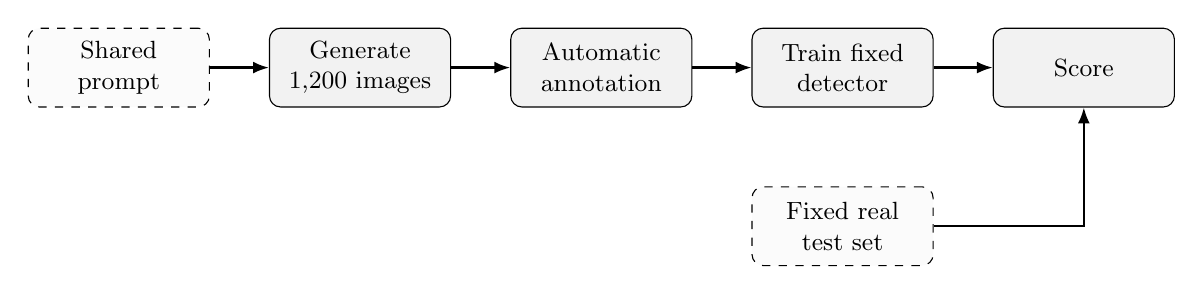
\begin{tikzpicture}[
  node distance=0.45cm and 0.75cm,
  stage/.style={rectangle, draw, rounded corners, fill=gray!10, minimum width=2.3cm, minimum height=1.0cm, align=center, font=\small},
  fixed/.style={rectangle, draw, dashed, rounded corners, fill=gray!3, minimum width=2.3cm, minimum height=1.0cm, align=center, font=\small},
  arr/.style={-{Latex[length=2mm]}, thick}
]
\node[fixed] (p) {Shared\\prompt};
\node[stage, right=of p] (g) {Generate\\$1{,}200$ images};
\node[stage, right=of g] (l) {Automatic\\annotation};
\node[stage, right=of l] (t) {Train fixed\\detector};
\node[fixed, below=1.0cm of t] (r) {Fixed real\\test set};
\node[stage, right=of t] (s) {Score};
\draw[arr] (p) -- (g);
\draw[arr] (g) -- (l);
\draw[arr] (l) -- (t);
\draw[arr] (t) -- (s);
\draw[arr] (r.east) -| (s.south);
\end{tikzpicture}
\caption{One generator$\times$prompt-regime cell. Dashed boxes are shared across every cell and never vary. Only the generator (and, deliberately, the prompt regime) changes.}
\label{fig:generator-comparison-pipeline}
\end{figure}

Several of these controls are structural rather than procedural, which is what makes them credible. The prompt text is stored one level above any individual generator's output directory, so it is physically the same text for every model that runs a given regime and cannot drift per model. Annotation was deliberately postponed until every cell had been generated, so that a single pass covers all of them under identical rules rather than each cell being annotated under whatever conventions happened to hold when it was produced. Category identifiers are taken unchanged from the real test set instead of being renumbered per cell, so every cell is scored in exactly the same label space. Each cell's synthetic images are training data by construction, with no synthetic image ever entering evaluation. Finally, the training code for this sub-study is a copy of the main pipeline rather than an import of it, so the comparison cannot silently change behavior when the main $225$-class pipeline is modified.

\Cref{tab:generator-comparison-factors} lists the two factors that do vary. The prompt regime is treated as a factor rather than an implementation detail for a reason developed in \Cref{sec:generator_comparison_prompts}. The candidate models differ by more than two orders of magnitude in how much text they can condition on, so holding the prompt constant and holding the conditioning constant are not the same thing. A naive comparison would therefore confound generative quality with prompt capacity.

\begin{table}[H]
\centering
\caption{The two factors varied in the comparison. Everything else is a fixed control.}
\label{tab:generator-comparison-factors}
\begin{tabularx}{\textwidth}{@{}lX@{}}
\toprule
Factor & Levels \\
\midrule
Generator & Four API services and six locally-run open-weight models (\Cref{sec:generator_comparison_roster}) \\
Prompt regime & \texttt{full} (the unabridged production prompt), \texttt{compressed} (an identical short prompt every model can read), \texttt{maxlen} (each model's own maximum usable prompt length) \\
\bottomrule
\end{tabularx}
\end{table}

Each cell comprises $12$ classes $\times\ 100$ images $= 1{,}200$ synthetic training images. The per-class count was fixed in advance and applied uniformly: under-provisioning a single generator would bias its downstream result in a way no later analysis could repair. Conditioning is zero-shot text-to-image throughout (no generator was given reference images). Supplying visual examples to some models and not others would confound the models' prior knowledge of a species with few-shot assistance.

%%%%%%%%%%%%%%%%%%%%%%%%%%%%%%%%%%%%%%%%%%%%%%%%%
\subsection{Class-Subset Selection}\label{sec:generator_comparison_classes}

The subset must expose three distinct phenomena. First, long-tail species that are plausibly under-represented in the generators' own pretraining data, which test whether a model can render a species it has rarely seen from a textual description alone. Second, classes with enough real test images for a downstream accuracy difference to be distinguishable from noise. Third, visually near-identical species, which test whether synthetic data can teach the fine-grained diagnostic markers on which species-level discrimination depends.

These pull against each other, and the tension is worth stating plainly rather than hiding: the rarest species (the best probes for absent prior knowledge) are precisely those with the fewest real test images, and therefore the worst probes for downstream statistical power. The subset resolves this by covering all three properties \emph{as a set} rather than in every class. A few rare species that nonetheless clear a useful test-set size are included specifically to decouple rarity from test-set size. The genuinely test-limited rare species are carried instead for the qualitative and per-image automatic measures, which have sample size at the image level, rather than for their downstream accuracy.

\Cref{tab:generator-comparison-classes} lists the resulting $12$ classes. The rarity proxy is the per-species image count recorded in the GBIF survey used for class selection (\Cref{sec:target_class_definition}). Because that survey caps at approximately $300$ images per taxon, a count at the ceiling means only \enquote{at least $300$}, whereas a low count indicates genuine scarcity rather than a sampling artifact.

\begin{table}[H]
\centering
\caption{The $12$-class comparison subset, grouped by the property each class contributes. \enquote{Real test} is the number of real photographs used to score every cell. \enquote{GBIF} is the rarity proxy, capped near $300$.}
\label{tab:generator-comparison-classes}
\begin{tabularx}{\textwidth}{@{}lllrrX@{}}
\toprule
Class & Band & Group & Real test & GBIF & Contribution \\
\midrule
Plains zebra & D & Look-alike & $2{,}079$ & $\geq 300$ & Broad stripes with brown shadow stripes \\
Grévy's zebra & B & Look-alike & $224$ & $84$ & Narrow dense stripes, white belly \\
Mountain zebra & D & Look-alike & $467$ & $173$ & Gridiron rump pattern, dewlap \\
\midrule
Red fox & D & Anchor & $2{,}150$ & $\geq 300$ & Ubiquitous. Any capable model should succeed \\
American black bear & D & Anchor & $2{,}097$ & $\geq 300$ & Large, common, well represented \\
Lion & D & Anchor & $2{,}097$ & $\geq 300$ & Iconic. A sanity ceiling for every model \\
\midrule
Kinkajou & A & Rare & $160$ & $294$ & Rare but test-robust \\
Water deer & A & Rare & $151$ & $204$ & Rare but test-robust. Tusks, no antlers \\
Ringtail & A & Rare & $186$ & $300$ & Rare but test-robust. Banded tail \\
Saiga & A & Rare & $50$ & $58$ & Distinctive proboscis. Test-limited \\
Aye-aye & A & Rare & $29$ & $29$ & Extreme morphology. Test-limited \\
Pangolin family & A & Rare & $52$ & $1$--$63$ & Scaled body, exotic texture. Test-limited \\
\bottomrule
\end{tabularx}
\end{table}

Because this experiment never trains on real images, the real photographs that the production split reserves for training and validation are idle here and were folded into the test set for Band B, C and D classes, substantially increasing statistical power for the anchor classes in particular. Band A classes, whose real images are already entirely allocated to testing (\Cref{sec:band_structure}), are unaffected. One consequence must be acknowledged. The production split assigns training images greedily by quality score and validation images from the middle of the quality distribution, whereas its test images were sampled without that bias. Folding all three together therefore skews the enlarged test set toward higher image quality than a random sample of the class pool. This does not bias the comparison between generators, since every generator is scored on the identical enlarged set, but it does mean this test set is specific to this sub-study and is not the project's general real-image benchmark. The full pool comprises $9{,}742$ real photographs. The class list was frozen to a file before any image was generated, following the same freeze-then-run discipline used for the dataset splits.

%%%%%%%%%%%%%%%%%%%%%%%%%%%%%%%%%%%%%%%%%%%%%%%%%
\subsection{Generator Roster}\label{sec:generator_comparison_roster}

Candidates were drawn from two tiers with different cost structures and different licensing implications: proprietary services billed per image, and open-weight models run locally on project hardware at the cost of GPU time only. \Cref{tab:generator-api-roster} lists the API tier and \Cref{tab:generator-local-roster} the local tier.

\begin{table}[H]
\centering
\caption{API generators included in the comparison, and the candidates excluded with their reasons.}
\label{tab:generator-api-roster}
\begin{tabularx}{\textwidth}{@{}lX@{}}
\toprule
Model & Role or reason for exclusion \\
\midrule
\texttt{gemini-3.1-flash-image-preview} \cite{GeminiAPI} & The production incumbent. Its \texttt{full}-regime images already existed \\
\texttt{gemini-3.1-flash-lite-image} & The same vendor's cheaper tier. Tests whether the incumbent's price buys quality \\
\texttt{gpt-image-2} (low) \cite{ImageGenerationOpenAI} & Cross-vendor price floor \\
\texttt{gpt-image-2} (medium) & Quality-tier contrast against \texttt{low} at matched prompt \\
\midrule
\texttt{gpt-image-2} (high) & Excluded: roughly an order of magnitude above the incumbent's per-image cost \\
Nano Banana Pro & Intended as the quality ceiling. Never generated: the most expensive site and the least decision-relevant, since training data would not be produced at that price regardless \\
Imagen 4 & Excluded: withdrawn from the vendor's API during the study \\
Midjourney & Excluded: no official API. Unofficial clients breach the terms of service \\
Adobe Firefly & Excluded: the cleanest data provenance of any candidate, but only via an enterprise contract far beyond the project budget \\
FLUX API & Excluded: its terms restrict training models on its outputs and sell synthetic-data rights separately \\
\bottomrule
\end{tabularx}
\end{table}

The FLUX API exclusion is worth noting explicitly, because it is the same category of reasoning that governs image licensing in \Cref{sec:candidate_sources_licensing}: a service whose terms forbid training on its outputs is unusable for this purpose regardless of output quality, and no amount of visual inspection would have revealed that.

\begin{table}[H]
\centering
\caption{Locally-run open-weight generators. \enquote{Offload} indicates whether the model had to stream weights between host and device memory to fit the available $23.8\,\mathrm{GB}$ of video memory.}
\label{tab:generator-local-roster}
\begin{tabularx}{\textwidth}{@{}lXllc@{}}
\toprule
Model & Scale & License & Precision & Offload \\
\midrule
RealVisXL + SDXL-Lightning \cite{podellSDXLImprovingLatent2023} & SDXL-scale, $4$-step distilled & OpenRAIL++ & fp16 & No \\
Stable Diffusion 3.5 Medium \cite{esserScalingRectifiedFlow2024} & $2.5\,\mathrm{B}$ transformer & Stability Community & bf16 & No \\
Stable Diffusion 3.5 Large & $8\,\mathrm{B}$ transformer & Stability Community & bf16 & Yes \\
Stable Diffusion 3.5 Large Turbo & $8\,\mathrm{B}$, $4$-step distilled & Stability Community & bf16 & Yes \\
FLUX.2-klein \cite{labsBlackForestLabs} & $9\,\mathrm{B}$ transformer, $4$-step distilled & FLUX non-commercial & bf16 & Yes \\
HiDream-I1 \cite{HiDreamaiHiDreamI1FullHugging2025} & $17\,\mathrm{B}$ transformer, four text encoders & MIT (composite) & NF4 & Yes \\
\midrule
Qwen-Image \cite{QwenQwenImageHugging2025} & $20.4\,\mathrm{B}$ transformer & Apache-2.0 & NF4 & Dropped \\
FLUX.2-dev & $32\,\mathrm{B}$ transformer & FLUX non-commercial & --- & Rejected \\
\bottomrule
\end{tabularx}
\end{table}

The composition of this roster is the outcome of a sequence of decisions that are more informative than the final list. \textit{FLUX.2-dev} was evaluated first as the strongest available open model and rejected on memory grounds: even its pre-quantised four-bit community checkpoint totals roughly $34\,\mathrm{GB}$ of weights against $23.8\,\mathrm{GB}$ of video memory, making weight streaming mandatory and an out-of-memory failure a live risk. \textit{FLUX.2-klein} replaced it. The reason is not a smaller footprint (it is also approximately $34\,\mathrm{GB}$ and also streams), but step distillation: at four denoising steps rather than twenty-eight to fifty, it pays the streaming penalty an order of magnitude fewer times per image.

\textit{HiDream-I1} was initially rejected and later readmitted, and the episode is recorded here because it changed how model availability was verified. It requires a gated third-party language model as its fourth text encoder, which is not bundled with it. An initial access check failed with a live authorisation error. A metadata query against the same repository had reported the gate as satisfiable, which it was not. Availability was thereafter confirmed instead by actually downloading a file rather than by querying metadata. When access was subsequently granted, the model was admitted. Its footprint made it the most constrained model onboarded: at full precision its components total roughly $63.5\,\mathrm{GB}$, more than the host's memory, and because weight streaming loads the entire pipeline into host memory before moving parts to the device, a naive load risked failing before generation began. Quantising its two largest components to four-bit brought resident memory to roughly $25.5\,\mathrm{GB}$, which fits the host while still exceeding device memory. Streaming therefore remained mandatory regardless.

\textit{Qwen-Image} was the roster's most permissively licensed candidate and was dropped nonetheless. Because no pre-quantised checkpoint exists for it, it had to be quantised to four-bit at load time, and inspection of its benchmark output showed visible quantisation artifacts (stippled noise in flat regions such as sky and grass) that the other quantised model did not exhibit. Since it had been retained primarily for its license rather than its output, and since the artifact is structural to the quantisation this hardware requires rather than a property of the model at full precision, its full run was canceled before committing the approximately $34$ hours of GPU time it would have cost. This is stated as a limitation rather than a finding: the comparison contains no evidence about Qwen-Image at full precision.

Licensing was tracked for the local tier as it was for image sources. Two models carry genuinely permissive licenses. The remainder carry community or non-commercial terms that would need review before any production use, and HiDream-I1's nominally permissive license is in practice a composite that inherits the terms of its gated text encoder. For a comparison whose purpose is to inform a commercial product, a model's license is part of its score, not a footnote to it.

%%%%%%%%%%%%%%%%%%%%%%%%%%%%%%%%%%%%%%%%%%%%%%%%%
\subsection{Prompt Regimes}\label{sec:generator_comparison_prompts}

The production prompts are long: approximately $1{,}300$ words of species description, behavior, habitat, scene specification, photography style and explicit requirements. The SDXL-family text encoder stops reading after $77$ tokens \cite{radfordLearningTransferableVisual2021}, roughly $50$ words. Handing both models the same text therefore does not give them the same information, and a quality gap measured that way would confound two distinct causes: how well a model generates, and how much it was allowed to condition on. \Cref{tab:generator-prompt-regimes} defines the three regimes used to separate them.

\begin{table}[H]
\centering
\caption{The three prompt regimes and what each is for.}
\label{tab:generator-prompt-regimes}
\begin{tabularx}{\textwidth}{@{}llX@{}}
\toprule
Regime & Budget & Purpose \\
\midrule
\texttt{full} & $\approx 1{,}300$ words & Each API model at its maximum usable prompt. Reproduces production conditions \\
\texttt{compressed} & $\leq 75$ tokens & An \emph{identical} prompt every model can read in full. The apples-to-apples condition \\
\texttt{maxlen} & $75 / 256 / 512$ tokens & Each local model at its own encoder's capacity. The best each can actually do \\
\bottomrule
\end{tabularx}
\end{table}

The \texttt{compressed} prompt is dense and ordered by importance, because the encoder weights early tokens most heavily and discards everything past its limit. Its slot order (species name, one to three diagnostic features, pose, habitat, then style anchors) is also a priority statement, made explicit by the trimming rule applied when a prompt exceeds budget. That rule drops habitat first, then pose, then reduces diagnostic features from three to two to one. The species name and at least one diagnostic marker are therefore the last elements to survive. Across all $1{,}200$ prompts the longest reached $57$ tokens against the $75$-token budget, verified with the target encoder's own tokeniser rather than estimated from word counts. Because the budget leaves no room for the six-axis scene grid used in production, only the pose varies across a class's images in this regime, with habitat fixed per class.

The \texttt{maxlen} regime pursues the opposite goal and uses the opposite construction. A first attempt truncated the \texttt{full} prompt to each model's budget and was abandoned after inspection. The prompt's structural sections alone total approximately $464$ words. These include scene specification, photography style and the numbered requirements, that is, everything which is not free-text species description. That is already more than the entire $256$-token budget before a single word of species description is added. The regime was instead built by accumulation rather than truncation, starting from a short template and adding description sentences until the next one would breach the budget, which is the exact inverse of the \texttt{compressed} regime's trimming cascade. Per-image pose and environment are carried over from the production image list, so the prompts retain genuine per-image variation rather than cycling a small fixed set. Measured across all $2{,}400$ generated prompts, the longest reached $245$ tokens in the $256$-token tier and $495$ in the $512$-token tier, both deliberately under their nominal ceilings to absorb the difference between the two related tokenisers that share the larger tier.

\Cref{fig:prompt-regime-example} illustrates the practical scale of the difference for a single class, which conveys the fairness problem more directly than any description of the builders.

\begin{figure}[H]
\centering
\begin{minipage}{0.95\textwidth}
\small
\textbf{\texttt{compressed}} ($150$ characters):
\begin{quote}\itshape
lion, tawny uniform coat, tufted tail, muscular shoulders, standing alert, on open savanna grassland, wildlife photograph, telephoto, photorealistic, full body
\end{quote}
\textbf{\texttt{maxlen}, $256$-token tier} (excerpt):
\begin{quote}\itshape
Realistic wildlife photograph of a lion (panthera leo). Species characteristics: tawny uniform coat, tufted tail, muscular shoulders. The lion is a muscular, broad-chested cat with a short, rounded head\ldots{} The lion trots along a game trail, its body fluid and powerful as it investigates a scent. A sun-bleached savanna with golden tall grass\ldots{} Exactly one lion in frame, diagnostic features clearly visible, no other individuals of the same species.
\end{quote}
\textbf{\texttt{full}} ($4{,}642$ words): task framing, verbatim species description, natural behavior and habitat, a six-axis scene specification, photography style, and eight numbered critical requirements.
\end{minipage}
\caption{The same class under the three prompt regimes. The content is matched (the same species facts are expressed throughout), and only the verbosity changes. The contrast measures how much text a model can use rather than what the text says.}
\label{fig:prompt-regime-example}
\end{figure}

Two asymmetries remain and are disclosed rather than smoothed over. First, the \texttt{full} regime is not byte-identical across vendors: one API caps prompts at $32{,}000$ characters, which several species with long encyclopedia articles exceed, so their free-text description was trimmed in the request while the generation-critical scene specification and requirements were left intact. Second, negative prompts could not be applied uniformly, because the FLUX-family pipeline accepts no plain-text negative prompt at all. Rather than forcing parity by removing a capability the other models genuinely have, negative prompts were treated as a model-native affordance and documented as such. However, one cell consequently lacks a control the others have.

Reproducibility differs between the tiers in a way that cannot be engineered away. The local models are fully deterministic: per-image seeds are derived from a fixed class ordering, so they remain stable regardless of which subset of classes a given run covers. The API services do not expose a seed, so their exact images cannot be regenerated. For those cells, the archived images, together with the recorded model identifier, request parameters and submission time, are the reproducible artifact. One further caveat applies within the local tier: the \texttt{compressed} and \texttt{maxlen} regimes index their seeds differently, so an image occupying the same slot in the two regimes was not generated from the same seed. The two regimes are therefore internally reproducible but not seed-matched to each other, which adds noise to any direct comparison between them.

%%%%%%%%%%%%%%%%%%%%%%%%%%%%%%%%%%%%%%%%%%%%%%%%%
\subsection{Throughput, Cost and Hardware}\label{sec:generator_comparison_cost}

Generation ran on a single NVIDIA A40 virtual GPU instance with $23.8\,\mathrm{GB}$ of video memory and $47\,\mathrm{GB}$ of host memory. Detector training ran separately on an RTX 3060. Throughput is reported as a first-class result rather than as background detail, because a generator that produces excellent images at an unusable rate is not a practical source of training data. \Cref{tab:generator-throughput} gives the measured wall-clock cost of each complete $1{,}200$-image cell.

\begin{table}[H]
\centering
\caption{Measured generation cost per complete $1{,}200$-image cell. Every local cell completed with zero failures. API costs are the amounts actually billed.}
\label{tab:generator-throughput}
\begin{tabular}{@{}lrr@{}}
\toprule
Generator & Seconds per image & Cost per cell \\
\midrule
RealVisXL + SDXL-Lightning & $0.93$ & $0.31\,\mathrm{h}$ \\
Stable Diffusion 3.5 Medium & $23.94$ & $7.98\,\mathrm{h}$ \\
Stable Diffusion 3.5 Large Turbo & $24.82$ & $8.27\,\mathrm{h}$ \\
FLUX.2-klein & $31.19$ & $10.40\,\mathrm{h}$ \\
Stable Diffusion 3.5 Large & $54.34$ & $18.11\,\mathrm{h}$ \\
HiDream-I1 & $143.92$ & $47.97\,\mathrm{h}$ \\
\midrule
\texttt{gpt-image-2} (low), \texttt{full} & --- & $\$10.11$ \\
\texttt{gpt-image-2} (medium), \texttt{full} & --- & $\$29.36$ \\
\texttt{gemini-3.1-flash-image-preview} & --- & $\approx$~\texteuro$48$ \\
\bottomrule
\end{tabular}
\end{table}

The six local cells consumed approximately $93$ GPU-hours in total. This figure is itself relevant to the thesis's practicability question: generating the full $12{,}600$-image production set locally, rather than the $1{,}200$-image comparison subset, would have taken weeks of continuous GPU time on this hardware, which is a substantial part of why an API service was the practical choice for production irrespective of output quality.

Two observations about these measurements are worth recording. First, small-sample benchmarks proved unreliable predictors in both directions: the two models whose \texttt{maxlen} prompts are longest ran materially slower than their short-prompt benchmarks suggested, because prompt length has a real and measurable encoding cost, while two others ran faster because their benchmarks were contaminated by cold-start overhead. Second, an investigation into why device memory utilisation sat between $23\%$ and $39\%$ found that weight streaming had been applied to every model as a blanket default inherited from a script targeting a $12\,\mathrm{GB}$ card. Removing it for the one model that comfortably fits without it produced a $1.8\times$ speed-up ($27.33$ to $14.84$ seconds per image), confirmed by re-measurement. The finding does not generalize: the four largest models exceed device memory before activations are counted, so they retain streaming and have no headroom to reclaim.

The API cost figures also carry a lesson that is not visible from published price lists. The cheapest tier's measured cost was roughly $2.8$ times its naive estimate, because prompt text is billed as input tokens separately from image generation, and the \texttt{full} regime's long prompts add an approximately fixed per-image surcharge. For long-prompt workloads, prompt length is a cost driver and not only a quality lever.

%%%%%%%%%%%%%%%%%%%%%%%%%%%%%%%%%%%%%%%%%%%%%%%%%
\subsection{Annotation, Detector and Training Protocol}\label{sec:generator_comparison_training}

Every cell was annotated by the same detector \cite{beeryEfficientPipelineCamera2019} and procedure used for the production synthetic images (\Cref{sec:synthetic_annotation}), with identical detection thresholds, so that the comparison audits exactly the kind of ground truth that the production pipeline ships. One deviation must be stated clearly, because it qualifies every downstream number reported in \Cref{sec:results_synthetic_data_practicability}: the human review stages of that procedure were never executed for this sub-study, so all cells use the automatic detector's own boxes under the documented best-effort fallback. The consequence is that the comparison is provisional. It is the best comparison currently obtainable, and the relative ranking is unlikely to be an artifact of annotation since every cell was annotated identically, but the absolute accuracy figures are not final.

The proportion of images for which the detector found exactly one adequately sized animal is itself reported as a quality signal rather than treated as bookkeeping, since a low yield indicates malformed or ambiguous subjects and also imposes a real annotation cost. Across the local cells this ranged from $93.6\%$ to $98.8\%$, with essentially no images containing no detectable animal at all.

\textit{YOLO26n} \cite{UltralyticsYOLO262025} was fixed as the detector for every cell. The alternative already available in the project was \textit{YOLOv5s} \cite{ultralyticsComprehensiveGuideUltralytics}, and the choice between them is a choice about what question the experiment answers. \textit{YOLOv5s}, at $7.2\,\mathrm{M}$ parameters, is approximately the size of the detector already deployed in the production binocular pipeline, so a result obtained on it would answer \enquote{is this synthetic data good enough for the model that already ships}. \textit{YOLO26n}, at $2.4\,\mathrm{M}$ parameters, is the architecture class this thesis actually targets for embedded deployment, so a result obtained on it remains load-bearing for the main study. The usual objection to the smaller model is that a capacity-starved network cannot resolve differences between two reasonable datasets. This does not apply at this scale. Each cell trains on $1{,}200$ images across $12$ classes from pretrained weights, a regime in which neither model is remotely capacity-limited. The binding constraint here is instead the transferability of the synthetic images' features, rather than parameter count. Training time was verified not to differ materially between the two, so it did not enter the decision.

Model selection and early stopping require held-out data, and the real test set is deliberately not it. A fifth of each cell's synthetic images is carved off as an internal validation split, stratified per class and drawn with a split seed independent of the training seed. The split is therefore identical across a cell's repeated runs, and only weight initialisation and batch ordering differ between them. The real test set is scored exactly once per run, at the end, on the best checkpoint. This serves two purposes: it prevents model selection from peeking at the set that produces the headline metric, and it avoids spending several minutes per epoch scoring $9{,}742$ images, which would otherwise dominate a run whose training step takes seconds.

Because a single training run on a dataset this small is noisy, each cell was trained repeatedly with different seeds and its results averaged. In the final state every API cell has three seeds and every local cell two, short of the three that the protocol itself recommends for the local tier. \Cref{sec:results_synthetic_data_practicability} shows why this matters in practice.

%%%%%%%%%%%%%%%%%%%%%%%%%%%%%%%%%%%%%%%%%%%%%%%%%
\subsection{Evaluation Methodology}\label{sec:generator_comparison_evaluation}

The objection this sub-study answers was to a single informal judgment. The remedy is not to abandon qualitative evaluation but to make it structured, blind and multi-rater, and to triangulate it against two quantitative axes that do not depend on human impression. A generator's standing is reported on all three, and a claim is strong only when they agree. \Cref{tab:generator-evaluation-axes} summarises the three axes together with what was actually carried out, since the gap between the two is material to how the results should be read.

\begin{table}[H]
\centering
\caption{The three evaluation axes as designed, and their execution status.}
\label{tab:generator-evaluation-axes}
\begin{tabularx}{\textwidth}{@{}lXl@{}}
\toprule
Axis & Instrument & Executed \\
\midrule
A -- Qualitative & Blind, multi-rater rubric with inter-rater agreement & No \\
B -- Automatic proxies & Teacher recognition, FID/KID, CLIP-score, annotation yield & Yield only \\
C -- Downstream utility & Detection accuracy on real photographs & Yes, all $12$ cells \\
\bottomrule
\end{tabularx}
\end{table}

\paragraph{Axis A -- Structured Qualitative Rubric}
Each generated image, or a fixed random sample per class and model, is scored on six pre-registered criteria. The first two are anatomical correctness (limb count, proportions, absence of fused or duplicated parts) and diagnostic-feature fidelity (whether the species-defining markers are present and correct). Species identity (whether a knowledgeable observer would name the intended species rather than a generic relative) is the third. The remaining three criteria are habitat plausibility, photorealism, and a binary or counted artifact rate covering text, watermarks, extra animals and impossible geometry. What makes this thesis-grade rather than impressionistic is the protocol around it: model identity is hidden and presentation order is randomised, and at least two and preferably three independent raters are used. An inter-rater agreement statistic is reported alongside the scores rather than relegated to a footnote. The rubric is also frozen before any output is examined, so that the criteria cannot be reverse-engineered toward a preferred model. This axis is the only instrument in the study capable of separating generators on the rare classes. As \Cref{sec:results_per_class_structure} shows, downstream accuracy is uniformly at a noise floor in these classes. It was specified in full and not executed within the time available, which is recorded here as a named limitation rather than omitted.

\paragraph{Axis B -- Automatic Proxies}
Four measures were specified, each scaling to every image and therefore supplying the statistical power the rare classes lack. The primary one is teacher-recognition confidence: running the project's own classifier \cite{gadotCropNotCrop2024a} over the generated images asks directly whether the model that would act as a distillation teacher recognizes the intended species, and with what confidence, which is close to a direct measurement of whether the diagnostic features are present. The remaining three are per-class Fréchet and kernel distances against the real images of the same class \cite{heuselGANsTrainedTwo2018,binkowskiDemystifyingMMDGANs2021}, computed per class because a global score conceals per-species failure. The second is a CLIP-based image--prompt alignment score for prompt adherence \cite{hesselCLIPScoreReferencefreeEvaluation2021}, computed with an encoder used by none of the generators. The third is the automatic annotation yield already described. Only the last of these was computed. The absence of the other three is a real gap, and it is the reason the results chapter leads with downstream accuracy rather than with a converged multi-axis judgment.

\paragraph{Axis C -- Downstream Utility}
The fixed detector is trained on each cell's synthetic images and evaluated on real photographs only, never on synthetic ones, consistent with the evaluation policy set out in \Cref{sec:evaluation_framework}. The headline measure is mean average precision over the real test set. Alongside it, two finer measures address the subset's design: per-class average precision, which separates the data-rich anchors from the rare classes; and the within-group confusion rate over the three zebra species, defined as the fraction of correctly localised detections that land in the right look-alike group but are assigned the wrong species. That last measure is the sharpest available test of whether synthetic data can teach species-level discrimination at all. Of the frozen look-alike groups (\Cref{sec:gt_annotation_integrity}), only the zebras have more than one member inside this $12$-class subset, so the bear group's confusion rate is structurally zero and is excluded as carrying no signal rather than reported as a perfect score.

\paragraph{Decision Rule}
Fixing the criterion in advance matters as much as fixing the rubric. A generator counts as usable if it lands within a stated margin of the incumbent on the axes that matter (downstream accuracy on real photographs and diagnostic fidelity) \emph{and} is practical on cost and throughput. Raw photorealism alone is explicitly not sufficient, since it is precisely the impression that motivated the original unjustified choice. Correspondingly, the production choice is justified only if the incumbent sits at or near the top on those axes. Because differences between cells on a dataset this small may fall within run-to-run noise, no winner is declared from a single run: results are reported as a mean with its spread across seeds, and two cells whose intervals overlap are reported as indistinguishable rather than ranked.

%%%%%%%%%%%%%%%%%%%%%%%%%%%%%%%%%%%%%%%%%%%%%%%%%
\section{Model Training and Experiment Tracking}\label{sec:model_training_experiment_tracking}

\Cref{sec:data_augmentation} fixed what a training run is shown. This section fixes everything else: which models are trained, the optimization protocol they share, the procedure that produced the frozen teacher, and the loss through which that teacher reaches the student. The distilled and the directly fine-tuned run must differ in the training signal and in nothing else.

%%%%%%%%%%%%%%%%%%%%%%%%%%%%%%%%%%%%%%%%%%%%%%%%%
\subsection{Model Selection}\label{sec:model_selection}

Two detector architectures are trained, and practical constraints rather than a comparative architecture search decide both. \textit{YOLOv5s} \cite{ultralyticsComprehensiveGuideUltralytics}, at $7.63\,\mathrm{M}$ parameters and $17.7$ GFLOPs at $640$ px, is the production-baseline reference, because it is approximately the size of the detector already deployed in the \textit{AX Visio} pipeline. It is commercially usable only up to commit \texttt{5cdad89} (\Cref{sec:lit_yolo_family}), which fixed the revision trained here. It is deliberately not the distillation student, since distilling into a model the size of what already ships studies no capacity reduction. \textit{YOLO26n} \cite{UltralyticsYOLO262025}, at $2.71\,\mathrm{M}$ parameters and $6.8$ GFLOPs, is the student. It is trained twice, once directly and once under distillation, and those two runs are the work's central comparison. The teacher is the \textit{MegaDetector} \cite{beeryEfficientPipelineCamera2019} and \textit{SpeciesNet} \cite{gadotCropNotCrop2024a} pipeline of \Cref{sec:lit_md_speciesnet}, which is wildlife-specific and, at roughly $193\,\mathrm{M}$ parameters, far too large to deploy.  % 140.06 M + 52.71 M, reports/embedded_benchmark/latency_summary.csv Nano-scale detectors outside the YOLO family were surveyed and set aside on time grounds, so neither student won a benchmarked comparison, a limitation carried in \Cref{sec:limitations}.

%%%%%%%%%%%%%%%%%%%%%%%%%%%%%%%%%%%%%%%%%%%%%%%%%
\subsection{Training Procedure}\label{sec:training_procedure}

Both detectors run the same optimization protocol, summarized in \Cref{tab:training-protocol}, and share the dataloader and augmentation code path without modification, which makes the byte-identical claim of \Cref{sec:augmentation_reproducibility} literal. The training and validation splits merge the synthetic imagery of \Cref{sec:band_structure} into the real imagery. The test split stays real, so the synthetic test set of \Cref{sec:synthetic_test_set} enters evaluation only where \Cref{sec:evaluation_framework} says it does.

\begin{table}[H]
\centering
\caption{Optimization protocol shared by both detector architectures.}
\label{tab:training-protocol}
\begin{tabularx}{\textwidth}{@{}lX@{}}
\toprule
Setting & Value \\
\midrule
Classes and input size & $225$ classes, $640 \times 640$ letterboxed \\
Optimizer & SGD, momentum $0.937$, Nesterov, weight decay $5 \times 10^{-4}$ applied to convolution weights only \\
Base learning rate & $1 \times 10^{-3}$, one tenth of a from-scratch rate, since every run starts from COCO-pretrained weights \\
Schedule & One-cycle, stepped per batch: $3$ warmup epochs to a peak of $1 \times 10^{-2}$, then cosine annealing to $1 \times 10^{-5}$ \\
Epoch ceiling & $200$, a safety bound, not a target \\
Early stopping & Patience of $20$ evaluations without a gain of $0.001$, gated until after warmup \\
Selection metric & mAP@[.5:.95] on the validation split \\
Weight averaging & Exponential moving average, checkpointed in place of the raw weights \\
Numerical precision & Automatic mixed precision on CUDA \\
Seed & $42$, fixed across all generators and dataloader workers \\
\bottomrule
\end{tabularx}
\end{table}

Two settings are exempted, and each exemption is a correctness requirement. Batch size is a property of an architecture's memory footprint, so it is determined per model by probing until allocation fails. The loss gains are the more consequential exemption. \textit{YOLO26n} is anchor-free and suppression-free, assigns targets through a task-aligned assigner, and carries no objectness term, so the anchor-based objectness, anchor-threshold and focal-loss gains tuned for \textit{YOLOv5s} have no counterpart in it. Transplanting them onto a structurally different loss would mis-scale the comparison, so each architecture keeps its own reference defaults.

One metric decides both which checkpoint is retained and when the run stops, which removes the temptation to select on one quantity and report another. Its binding cost is the validation pass, single-threaded over $225$ classes at roughly $12.5$ minutes regardless of image size or batch size against roughly $50$ minutes for a training epoch, so the evaluation interval is a tunable and patience counts evaluations, not epochs.  % scripts/training/yolo26n/model_exports/yolo26n-bs32-20260910-212812/
The runs reported in \Cref{chapter:results} validated every epoch and ran for between $182$ and $200$ epochs over four to nine days on a single \textit{NVIDIA A40}.

%%%%%%%%%%%%%%%%%%%%%%%%%%%%%%%%%%%%%%%%%%%%%%%%%
\subsection{Teacher Fine-Tuning}\label{sec:teacher_finetuning}

The teacher is fine-tuned on this work's dataset and then frozen, which is the standard two-stage arrangement and here also a resource requirement, since an ensemble of roughly $193\,\mathrm{M}$ parameters cannot run inside a student training step. It is instead evaluated once, offline, and its predictions cached.

Only the classifier is fine-tuned. \textit{MegaDetector} is class-agnostic and already accurate on camera-style imagery, so there is limited headroom in adapting a localizer that does not name species. The classifier trains on the same annotation files the detectors do, so teacher and student see identical image, box and class triples and not merely identical splits. Its native taxonomy carries $2{,}498$ leaf labels, and a grouped cross-entropy sums the leaf probabilities belonging to each of the project's $225$ classes before taking the loss. For the $178$ species-level classes this reduces to ordinary cross-entropy, and it only does real work for the genus-level and family-level classes that several leaves map into.

Three deviations follow from the teacher being a classifier rather than a detector. It trains at $480$ px, its own native input resolution. It uses AdamW at $1 \times 10^{-4}$ rather than SGD, the ordinary convention for adapting a pretrained classification backbone. And macro F1 rather than mAP selects the checkpoint. One caveat attaches to any accuracy improvement reported for this fine-tune. Part of the corpus was admitted by agreeing with the pre-fine-tuning classifier (\Cref{sec:speciesnet_matching}), so the fine-tuned classifier is partly measured against its own earlier self and the improvement is optimistic by an unknown, probably small amount.

%%%%%%%%%%%%%%%%%%%%%%%%%%%%%%%%%%%%%%%%%%%%%%%%%
\subsection{Knowledge Distillation Loss}\label{sec:kd_loss}

Feature-based distillation, which aligns intermediate activations, is excluded at the outset. It presupposes spatially corresponding feature maps, which a two-stage teacher seeing $480$ px crops and a single-stage student with a dense multi-scale pyramid over the whole frame do not have. Response-based distillation \cite{hintonDistillingKnowledgeNeural2015} is used instead, because it consumes only the teacher's final class distribution and so is indifferent to the architectural mismatch \cite{gouKnowledgeDistillationSurvey2021}.

The teacher's output is projected onto the $225$-class space and cached once per training image, so the frozen teacher never executes inside the training loop. The cache holds one distribution per image, from the highest-confidence detection, so multi-animal images contribute a single teacher vector. Secondary detections were not used as extra pseudo-annotations, so distillation's supervision advantage in multi-animal scenes remains untested here.

Distillation acts on the student's classification branch alone. The task-aligned assigner produces a soft target score vector $\mathbf{y}_i$ at each anchor $i$, and at the foreground anchors $\mathcal{F}$ that vector is blended toward the teacher distribution before the binary cross-entropy term is taken:
\begin{equation}
    \tilde{\mathbf{y}}_i = (1 - \alpha)\,\mathbf{y}_i + \alpha\,\tau_T(\mathbf{p}), \qquad i \in \mathcal{F},
    \label{eq:kd-blend}
\end{equation}
where $\mathbf{p}$ is the image's cached teacher distribution and $\tau_T$ applies temperature $T$. Background anchors, and images with no cached teacher entry, keep the assigner's own targets. The defaults are $T = 4$ and $\alpha = 0.5$, and the blend is applied to the one-to-one head the architecture uses at inference, not to its auxiliary head.

Two approximations in \Cref{eq:kd-blend} are worth stating, because both weaken the teacher signal relative to the textbook formulation. The cache stores probabilities rather than logits, so temperature cannot be applied before the softmax. It is applied instead as a renormalization on the simplex, $\tau_T(\mathbf{p})_c \propto p_c^{1/T}$, which is exact only at $T = 1$ and otherwise approximates the intended softening. And because the teacher distribution is per-image while the blend is per-anchor, one vector is broadcast across all of an image's foreground anchors, which is correct for a single-animal image and a simplification for any other. Box regression receives no distillation signal at all, since the teacher's suppressed output and the student's anchor-free head share no box-distribution representation to align.

The capacity gap between the two models bounds what this design can be expected to achieve. At a parameter ratio of roughly $70$ to $1$, it sits far outside the ratios the distillation literature treats as empirically safe, and negative transfer under such a gap is a documented failure mode and not a remote possibility \cite{mirzadehImprovedKnowledgeDistillation2020}. A distilled student that fails to beat its directly fine-tuned counterpart is nonetheless treated in \Cref{sec:results_kd_basic_comparison} as a result to report rather than a defect to debug away.

%%%%%%%%%%%%%%%%%%%%%%%%%%%%%%%%%%%%%%%%%%%%%%%%%
\subsection{Experiment Tracking}\label{sec:experiment_tracking}

Every run logs its complete configuration to a self-hosted tracking server, together with the commit hash, the device and the realized split sizes, so a finished run is reconstructable from the record and not from the working tree. \Cref{sec:appendix_experiment_tracking} gives the setup and the on-disk run layout. Reproducibility rests on a single seed, fixed at $42$, which seeds the Python, NumPy and Torch generators, selects deterministic convolution algorithms, reaches each dataloader worker, and is reused for the evaluation subsampling and the bootstrap resampling of \Cref{sec:evaluation_framework}. What it does not fix is arithmetic. Two runs at different batch sizes or on different devices are not bit-identical, so the seed buys a comparable sample and not a reproducible float, which is the level every comparison in \Cref{chapter:results} relies on.

%%%%%%%%%%%%%%%%%%%%%%%%%%%%%%%%%%%%%%%%%%%%%%%%%
\section{Evaluation Framework}\label{sec:evaluation_framework}

Every model trained in \Cref{sec:model_training_experiment_tracking} is scored on one fixed instrument, and this section defines it. Two properties of this dataset make a single mean-average-precision figure insufficient on its own. Several classes are barely separable in a still frame, so a species-level slip and a wholly unrelated call are errors of very different severity that one number cannot distinguish. And the dataset ships two test domains rather than one, a real held-out set that is uneven across classes and a class-balanced synthetic set, which an aggregate figure silently blends. The literature surveyed in \Cref{sec:lit_evaluation_metrics} supplies the baseline instrument and the diagnostic vocabulary. What it does not supply, as \Cref{sec:lit_real_synthetic_evaluation} states, is a precedent for the headline condition adopted here, which is therefore argued for directly in \Cref{sec:mixed_default}.

%%%%%%%%%%%%%%%%%%%%%%%%%%%%%%%%%%%%%%%%%%%%%%%%%
\subsection{Evaluation Axes}\label{sec:evaluation_axes}

Four axes describe every number this work reports about detection accuracy. \textbf{Granularity} is the class resolution at which a detection is judged correct, at three levels. \texttt{detect} ignores the class entirely and asks only whether an animal was localized. \texttt{coarse} merges visually confusable classes into the groups of \Cref{sec:lookalike_groups}. \texttt{fine} is the full $225$-way judgment. \textbf{Test domain} is which held-out images the metric is computed over, either the mixed, real or synthetic test set of \Cref{sec:mixed_default}. \textbf{Training band} is the per-class property of how a class's training data was composed, Band A through Band D as defined in \Cref{sec:band_structure}. \textbf{Metric vector} is the COCO statistics themselves \cite{linMicrosoftCOCOCommon2015}.

Crossing all four naively produces $3 \times 3 \times 5 \times 12 = 540$ numbers, which is unreportable and mostly uninformative. The four axes do not play the same role. Band and test domain are the independent variables, since this work asks whether synthetic training data works and whether it transfers to real photographs, so crossing those two is the experiment. Granularity is an error decomposition rather than a fourth experiment, and the metric vector is a fixed instrument. That yields the organizing rule for \Cref{chapter:results}. One default cell carries the headline, every diagnostic varies exactly one axis away from it and reports mAP@[.5:.95] and mAP50, and the full twelve-statistic vector is filled only in the default cell and once per band. No figure crosses average recall or the object-size splits with band or granularity, since none would answer a question posed here.

Treating granularity as a decomposition is what makes the ladder informative. The three levels are nested upper bounds, since a detection judged correct at the fine level is necessarily correct at the coarse and detection levels:
\begin{equation}
    \mathrm{mAP}_{\text{detect}} \;\geq\; \mathrm{mAP}_{\text{coarse}} \;\geq\; \mathrm{mAP}_{\text{fine}} .
    \label{eq:granularity-ladder}
\end{equation}
The quantities of interest are the two gaps in \Cref{eq:granularity-ladder}. $\Delta_{\text{coarse}}$ is the drop from detection to coarse classification, the cost of naming a group. $\Delta_{\text{fine}}$ is the drop from coarse to fine, the cost of naming the exact species within that group. A large $\Delta_{\text{fine}}$ beside a small $\Delta_{\text{coarse}}$ is the signature of the look-alike problem, and is the expected failure mode for this dataset. A large $\Delta_{\text{coarse}}$ instead means cross-group confusion, which is a genuine failure. A low $\mathrm{mAP}_{\text{detect}}$ means the detector cannot localize at all. One scorer produces all three levels by remapping class identifiers, and merged duplicates are charged as false positives, so a coarse figure is penalized rather than inflated.

%%%%%%%%%%%%%%%%%%%%%%%%%%%%%%%%%%%%%%%%%%%%%%%%%
\subsection{The Mixed Real+Synthetic Default}\label{sec:mixed_default}

Three test domains are distinguished throughout this work, and the reporting rules below depend on telling them apart. The \textbf{real test set} is the held-out real photographs, uneven across classes by construction. The \textbf{synthetic test set} is the balanced $225 \times 50$ held-out set of \Cref{sec:synthetic_test_set}. The \textbf{mixed test set} is the union of the two, scored together as a single set, not averaged after the fact. The default cell carrying the headline is fine granularity on the mixed test set over all bands, reported with the full twelve-statistic vector.

Three reasons support that default. The fixed $50$ synthetic images per class give every class a consistent, controlled probe. That matters most for the Band A classes, which hold as few as five to thirty real test images and whose real-only accuracy is otherwise dominated by a handful of hard frames. For a Band D class with up to $500$ real test images, the same $50$ images are a small, constant addition. And the mixed set always contains the real evidence, so no model in this work is ever judged on synthetic images alone.

Because the synthetic contribution is fixed while the real contribution varies by two orders of magnitude, the synthetic share of a class's score is inversely related to how much real data that class has. It is dominant for a thin Band A class and marginal for Band D. The real and synthetic test-image counts are therefore reported per class alongside the headline, and a synthetically trained class is partly scored on its own training domain under the mixed condition, a caveat \Cref{sec:results_band_granularity} states in full.

Two reporting rules follow, and both hold without exception. First, the real-only breakout is reported alongside the mixed headline every time. It is the primary-evaluation figure and the only number in this work comparable to a published real-image benchmark, and reporting it beside the headline is what prevents the synthetic component from quietly inflating a result. Second, the paired per-class difference between real and synthetic accuracy is monitored as a standing watchdog. Should that difference show the synthetic component systematically inflating or deflating the mixed figure, the default axes are to be revised. The likely revision is to make the real test set the default again and retain the mixed figure as secondary. \Cref{sec:results_domain_shift} states whether that trigger fired.

No comparison outside this work should read a $225$-class fine-grained wildlife mAP as equivalent to a published $80$-class COCO figure. The class count is larger and many of the classes are near-duplicates, so a lower fine-grained figure is expected and is not evidence of a weaker detector. The closest honest analog to a generic benchmark is the class-agnostic $\mathrm{mAP}_{\text{detect}}$, which measures localization independently of the taxonomy. All figures use COCO-standard settings, averaging over IoU thresholds from $0.5$ to $0.95$ with at most $100$ detections per image.

%%%%%%%%%%%%%%%%%%%%%%%%%%%%%%%%%%%%%%%%%%%%%%%%%
\subsection{Look-Alike Groups and Coarse Evaluation}\label{sec:lookalike_groups}

Coarse granularity needs a fixed table mapping each of the $225$ classes to a group. Grouping classes by the confusions a trained model makes is rejected outright, because a grouping derived from the model under evaluation is circular, and hand-listing the notorious look-alikes is subjective. A rollup to genus is reproducible and fixed before any model runs, so that taxonomic rollup is the backbone, corrected by a small documented override list. The construction follows the a-priori grouping principle of \textcite{hoiemDiagnosingErrorObject2012}, and the overrides exist because taxonomy leaks in both directions as a proxy for visual similarity.

The criterion is a judgment about what counts as a failure, not a technical rule. Two classes are merged when confusing them in a single still frame is a forgivable error, which belongs in $\Delta_{\text{fine}}$, and kept apart when confusing them is a real failure, which must surface in $\Delta_{\text{coarse}}$. Leopard and jaguar are therefore merged, since separating them from one still image is a specialist task. Lion and tiger are held in separate single-member groups despite sharing a genus. Where a case is uncertain the default is not to merge, since an unjustified merge silently forgives a real error. The resulting table holds $174$ groups, $30$ of them with more than one member, and $8$ overrides.  % reports/lookalike_groups_v2.csv
It is frozen before the first evaluation runs, because a later change would invalidate every coarse figure already computed without raising a visible error. \Cref{sec:results_lookalike_confusion} checks it against the confusions the model actually makes, descriptively and never as an input.

%%%%%%%%%%%%%%%%%%%%%%%%%%%%%%%%%%%%%%%%%%%%%%%%%
\subsection{Metric Selection}\label{sec:metric_selection}

The COCO twelve-statistic vector surveyed in \Cref{sec:lit_detection_metrics} is retained unchanged as the baseline instrument, because it is the bridge that keeps this work's numbers legible against published work. All scoring runs through one implementation, validated against the training loop's own evaluator, so a figure quoted from a training log and one quoted from an evaluation report are the same measurement.

Four qualifications accompany every number. Macro averaging over classes stays primary, as the COCO standard and the class-imbalance-robust choice, with a count-weighted average reported as a sensitivity check, since the two can diverge on a test set this uneven. Bootstrap confidence intervals, resampling images with replacement, cover the headline figure and the band and domain differences, because the Band A and Band B test sets are small enough that a difference between two models may not be a difference at all. The $9$ classes holding fewer than $30$ real test images are flagged in every per-class table, and the headline is reported both with and without them.  % scripts/training/yolo26n/model_exports/yolo26n-bs32-20260910-212812/evaluation/evaluation_report.json
And a single fixed seed governs every sampled evaluation, so re-running the suite against a new checkpoint yields a comparable figure.

Two instruments complement the metric vector without extending it. The error-type decomposition anchored in \Cref{sec:lit_error_decomposition} partitions the detector's mistakes into classification, localization, duplicate, background and missed ground truth, and corroborates that a coarse-to-fine gap really is look-alike confusion rather than a hidden localization problem. The within-group confusion rate asks, of the detections that are correctly localized and in the right group, what fraction name the wrong species. Both feed the reporting structure that \Cref{sec:results_regime_comparison} follows: a headline table per model, three diagnostic tables, and the per-class and full-vector material emitted as appendix artifacts.


    \newpage
\cleardoublepage
\chapter{Results}\label{chapter:results}

% TODO: lead-in paragraph stating the chapter's restructured weighting up
% front, mirroring the framing added to Chapter \ref{chapter:literature_review}.
% The headline results are (1) the practicability of synthetic training data,
% evaluated through the generator comparison of
% docs/synthetic-model-comparison (\Cref{sec:results_synthetic_data_practicability}),
% and (2) detection performance across the real/synthetic training-and-test
% regimes defined in docs/plans/2026-06-10_model-evaluation-strategy.md
% (\Cref{sec:results_regime_comparison}), since these are where the bulk of the
% thesis's actual experimental work went. Knowledge distillation and the
% embedded hardware check are demoted to a single smaller, explicitly-scoped-
% as-basic closing section (\Cref{sec:results_kd_and_embedded}), reflecting
% that only a single teacher/student comparison and a simple runtime check
% were carried out, not the fuller distillation-vs-direct-fine-tuning research
% program originally planned.

%%%%%%%%%%%%%%%%%%%%%%%%%%%%%%%%%%%%%%%%%%%%%%%%%
\section{Practicability of Synthetic Training Data: Generator Comparison}\label{sec:results_synthetic_data_practicability}
% TODO: reports the controlled comparison designed in
% docs/synthetic-model-comparison/01_experiment-design.md across the reduced
% class subset (docs/synthetic-model-comparison/02_class-selection.md) and the
% generator grid (docs/synthetic-model-comparison/03_api-models-landscape-and-pricing.md,
% 04_local-models-and-output-parameters.md): the incumbent
% \texttt{gemini-3.1-flash-image-preview}, other API models (gpt-image-2 at
% multiple tiers, Nano Banana 2 Lite/Pro), and local diffusion baselines
% (FLUX.1-schnell, RealVisXL+SDXL-Lightning, SD 3.5 Medium), each at full and
% prompt-length-compressed regimes where applicable
% (docs/synthetic-model-comparison/05_prompt-strategy-and-length-limits.md).
% Follows the three-axis methodology of
% docs/synthetic-model-comparison/06_evaluation-methodology.md.

\subsection{Qualitative Rubric Results}\label{sec:results_qualitative_rubric}
% TODO: blind, multi-rater scores per generator on the fixed rubric
% (anatomical correctness, diagnostic-feature fidelity, species identity,
% habitat plausibility, photorealism, artifact rate); report inter-rater
% agreement (Cohen's/Fleiss' kappa) alongside the scores, not as a footnote.

\subsection{Automatic Proxy Results}\label{sec:results_automatic_proxies}
% TODO: teacher-recognition confidence (SpeciesNet-on-synthetic top-1 and mean
% confidence) as the primary proxy, per-class FID/KID against real imagery,
% CLIP-score for prompt adherence, and MegaDetector auto-label yield per
% generator (a practicality signal, not just a quality one).

\subsection{Downstream Utility: Real-Test mAP per Generator}\label{sec:results_downstream_utility}
% TODO: the fixed detector/classifier trained on each cell's synthetic images,
% evaluated on the held-out real test set only (mixed and real-only
% breakouts per the evaluation strategy); the three-zebra-species fine-grained
% probe as the decisive look-alike test; per-generator €/image and
% images/hour alongside the accuracy numbers, following the single
% cross-axis ranking table sketched in
% docs/synthetic-model-comparison/06_evaluation-methodology.md \S7.

\subsection{Practicability Verdict}\label{sec:results_practicability_verdict}
% TODO: synthesize the three axes into a single practicability judgment --
% does the current generation of text-to-image models produce training data
% usable for this task at all, and was the production choice of Gemini
% justified against the alternatives on the axes that matter (real-test mAP
% and diagnostic fidelity), not merely on informal photorealism. This is the
% section that most directly answers the professor's original methodological
% objection (docs/synthetic-model-comparison/00_motivation-and-research-question.md).

%%%%%%%%%%%%%%%%%%%%%%%%%%%%%%%%%%%%%%%%%%%%%%%%%
\section{Detection Performance Across Training Regimes and Test Domains}\label{sec:results_regime_comparison}
% TODO: the thesis's other headline result, reporting the Tier 1/Tier 2
% structure of docs/plans/2026-06-10_model-evaluation-strategy.md \S9 for the
% YOLOv5s detector trained under the Band A-D data regimes
% (Methods \Cref{sec:band_structure}).

\subsection{Headline: Mixed Real+Synthetic mAP and the Real-Only Breakout}\label{sec:results_headline_mixed}
% TODO: Tier 1 table -- G=fine, D=mixed, B=all, full COCO-12 vector, alongside
% the real-only breakout (the public-comparison anchor) and the
% \texttt{mAP\_detect} class-agnostic analog (evaluation strategy \S7).

\subsection{Granularity Gap Decomposition}\label{sec:results_granularity_gaps}
% TODO: detect/coarse/fine mAP as a gap decomposition
% ($\Delta_{\text{coarse}}$, $\Delta_{\text{fine}}$, evaluation strategy \S4),
% backed by a TIDE error-type chart; interpret a large $\Delta_{\text{fine}}$
% with a small $\Delta_{\text{coarse}}$ as the expected look-alike-confusion
% signature for this dataset.

\subsection{Band $\times$ Granularity: Does Training Regime Change Accuracy?}\label{sec:results_band_granularity}
% TODO: the dataset's core scientific comparison -- the 4-band $\times$
% \{fine, coarse\} $\times$ \{mAP, mAP50\} grid (evaluation strategy \S6a),
% reported on the mixed domain with the real-only grid alongside it as the
% synthetic-vs-real-training tie-breaker, since Band A/B are partly scored
% on their own training domain under \texttt{mixed}.

\subsection{Domain-Shift Delta: Real vs.\ Synthetic Test Performance}\label{sec:results_domain_shift}
% TODO: the paired $\Delta_{\text{domain}}(\text{class}) = \text{mAP}_{\text{real}} -
% \text{mAP}_{\text{synthetic}}$ per class (evaluation strategy \S6b), reported
% as a distribution per band; this is also the watchdog check for the
% \texttt{mixed} default itself -- state explicitly whether the check passed
% (no revision of the default axes triggered) or whether a discrepancy emerged.

\subsection{Look-Alike Within-Group Confusion}\label{sec:results_lookalike_confusion}
% TODO: per-look-alike-group confusion table plus the block-diagonal confusion
% matrix restricted to the frozen look-alike groups
% (docs/plans/2026-06-11_lookalike-groups-review.md), using the same
% taxonomic-tolerance groups mined during ground-truth review
% (Methods \Cref{sec:gt_annotation_integrity}).

%%%%%%%%%%%%%%%%%%%%%%%%%%%%%%%%%%%%%%%%%%%%%%%%%
\section{Knowledge Distillation and Embedded Feasibility}\label{sec:results_kd_and_embedded}
% TODO: explicitly frame this section, in its opening paragraph, as
% intentionally reduced in scope relative to the original research question --
% a single basic comparison and a single runtime check, not an exploration of
% the wider design space surveyed in
% \Cref{sec:lit_knowledge_distillation,sec:lit_embedded_inference}. State the
% time-budget reason plainly rather than presenting the reduced scope as if it
% were the original plan.

\subsection{Distillation vs.\ Direct Fine-Tuning: A Single Basic Comparison}\label{sec:results_kd_basic_comparison}
% TODO: Setup A vs.\ Setup B (Methods \Cref{sec:augmentation_setups}), byte-identical
% augmentation pipelines, isolating the effect of the teacher signal alone;
% report the same headline mAP figure as \Cref{sec:results_headline_mixed} for
% both setups side by side. State clearly that this is one direct comparison
% at one teacher/student pairing, not a sweep over distillation strategies,
% temperature values, or teacher architectures.

\subsection{Runtime Benchmark on AX Visio Hardware}\label{sec:results_ax_visio_benchmark}
% TODO: the export pipeline used to get the trained YOLOv5s model onto the
% \textit{AX Visio} device, and the measured wall-clock inference
% latency/throughput (FPS) on-device; report it alongside the equivalent
% Raspberry Pi 5 proxy measurement to close the loop on the hardware-proxy
% reasoning of docs/2026-03-09_hardware-proxy-selection.md. State plainly
% whether the unoptimized model met a stated real-time threshold, since no
% quantization or other embedded optimization was applied -- this is a
% feasibility check, not an optimization result.

%%%%%%%%%%%%%%%%%%%%%%%%%%%%%%%%%%%%%%%%%%%%%%%%%
\section{Cross-Cutting Observations}\label{sec:results_general_observations}
% TODO: collects findings that don't belong to any single section above:
% training-time comparison across bands/setups; whether the synthetic-data
% practicability verdict (\Cref{sec:results_practicability_verdict}) is
% consistent with the band-comparison results
% (\Cref{sec:results_band_granularity}); an explicit closing statement that the
% knowledge-distillation and embedded-benchmark results
% (\Cref{sec:results_kd_and_embedded}) are preliminary/indicative given the time
% budget, setting up the Further Work section of Chapter
% \ref{chapter:discussion_conclusion} rather than being over-interpreted here.

    \newpage
\cleardoublepage
\chapter{Discussion and Conclusion}\label{chapter:discussion_conclusion}

\Cref{chapter:results} reported the measurements. This chapter reads them back against the four research questions of \Cref{sec:objective}, fixes what the evidence cannot carry, and proposes the work that follows from those limits. \Cref{sec:discussion} restates each question verbatim and answers it from the results chapter alone, without introducing new data. \Cref{sec:limitations} collects the boundaries and the one protocol deviation that bound every answer. \Cref{sec:further_work} maps each limitation onto a concrete follow-on, and \Cref{sec:conclusion} closes with what this work establishes.

%%%%%%%%%%%%%%%%%%%%%%%%%%%%%%%%%%%%%%%%%%%%%%%%%
\section{Discussion}\label{sec:discussion}

\Cref{sec:objective} posed four research questions. They are restated here verbatim and answered one at a time.

\begin{enumerate}
    \item Does knowledge distillation from a fine-tuned teacher model into a nano-scale student model yield higher detection accuracy than fine-tuning the same student directly on the wildlife dataset, given the domain shift from COCO-style classes to $225$ mammal species?
    \item Which synthetic-image generator produces the most useful training data for this domain, and do the two criteria available before any detector is trained, apparent visual realism and per-image price, predict that ranking?
    \item How does the composition of a class's training data, from synthetic images alone through a large pool of real photographs, affect detection accuracy, and does accuracy measured on the mixed test set hold up on the real test set alone?
    \item Does a nano-scale detector meet the per-frame latency budget of the target hardware without quantization or any other compression step, measured on a target-adjacent proxy device?
\end{enumerate}

\paragraph{Question $1$: Distillation Against Direct Fine-Tuning}
No, at the one design point that was tested. \Cref{sec:results_kd_basic_comparison} compares Setup A, which blends the frozen fine-tuned teacher's cached class distribution into the student's classification target at temperature $T = 4$ and weight $\alpha = 0.5$, against Setup B, which takes the assigner's own targets untouched. Direct fine-tuning is ahead in all $17$ reported cells of \Cref{tab:kd-vs-direct}. On the mixed test set it reaches a mAP of $0.599$ against the distilled student's $0.560$, and on the real test set $0.529$ against $0.479$. The margin is widest on Band A, whose supervision is entirely synthetic and thin, at $0.086$ mixed and $0.061$ real. That is the band the distillation hypothesis was expected to help most, so the negative answer holds on its own best case rather than only on aggregate.

Three properties bound how far that answer travels, and the first of them is a confound rather than a scope limit. The distilled run trained at an effective batch size of $16$ against $32$ for the direct run, both auto-reduced from a nominal $64$ by the memory probe, so batch size is a second varied factor whose contribution to the gap is unmeasured. The distilled run also ended early, at epoch $186$ of $200$ after a tracking-client exception, with its validation metric still rising from $0.724$ at epoch $175$ to $0.733$ at epoch $185$. The direct run stopped on its own patience criterion and was the more nearly converged of the two. Neither run carries a confidence interval, so the direction is treated as real and the magnitude as unquantified.

The scope limits are narrower still. One $(T, \alpha)$ point ran rather than the grid of \Cref{sec:kd_loss}, one teacher and student pairing was tested at a parameter ratio of roughly $72$ to $1$, and only response-based distillation was used. That ratio sits far outside the range the capacity-gap literature treats as safe, and it is a documented setting for negative transfer \cite{mirzadehImprovedKnowledgeDistillation2020}, so an unfavorable outcome there is closer to the expected case than to a refutation of the mechanism. The domain shift the question names as its premise was present by construction, since the student started from COCO weights and finished on $225$ mammal species, but its size is not measured anywhere in this work. The student's zero-shot baseline was never produced (\Cref{sec:results_general_observations}), so both setups are reported as absolute levels rather than as gains over the floor they shared. What the comparison rules out is a benefit from response-based distillation at $T = 4$ and $\alpha = 0.5$ with this pairing, and not knowledge distillation for this domain.

\paragraph{Question $2$: Which Generator, and Whether Realism or Price Predicts It}
\texttt{gpt-image-2} at its cheapest quality tier, conditioned on the unabridged \texttt{full} prompt regime, produced the most useful training data of the twelve cells compared, at $0.134 \pm 0.014$ mAP on the real test set (\Cref{tab:generator-ranking}). Neither criterion the question names predicts that ranking.

Apparent visual realism selected a reasonable generator that was not the best available one. The incumbent was chosen for the production synthetic dataset because its output looked more realistic, and it ranks third of twelve. \texttt{gpt-image-2} at its cheapest tier beats it by roughly $28\%$ under an identical prompt regime, and its own vendor's cheaper variant is statistically tied with it. Per-image price predicts nothing at all. The two \texttt{gpt-image-2} quality tiers differ by a factor of $2.9$ in price and are separated by $0.008$ mAP against a combined standard deviation of roughly $0.018$ (\Cref{sec:results_cost_vs_quality}). In the local grid the most expensive cell to produce, at nearly $48$ GPU-hours, ranks eleventh of twelve, while the cheapest by two orders of magnitude ranks twelfth. In neither vendor family is the cheaper tier the worse one, so generation cost is not usable as a proxy for training-data quality.

A third criterion the question did not anticipate outranks both. Compressing the prompt costs roughly half the downstream accuracy, at $-45\%$ and $-48\%$ for the two models of the controlled ablation in \Cref{tab:prompt-length-ablation}, and within-group confusion over the zebras rises in step. That effect is larger than most model-to-model differences in \Cref{tab:generator-ranking} and moves the top-ranked cell to fifth place. How much diagnostic detail a generator is given therefore matters more than which generator is chosen, across the range of models tested.

The ranking answers the question for data-rich classes and under the single evaluation axis that was executed. On the rare classes it answers nothing. Five of the six stay below $0.05$ average precision for every cell in the grid (\Cref{sec:results_per_class_structure}), and one generator draws kinkajous with a ringed tail and a spotted coat at no measured penalty (\Cref{fig:kinkajou-generator-samples}). The honest form of the answer is that the comparison ranks generators for well-photographed classes and establishes that its own instrument cannot rank them for the long-tail classes that motivated generating images in the first place.

\paragraph{Question $3$: Training-Data Composition, and Whether Mixed Accuracy Holds Up}
Composition matters, and it matters non-linearly. Bands A, B and C share an equal $200$-image training budget and differ only in what those images are, and \Cref{tab:band-grid-real} reports them on the real test set. Replacing half of a small real training set with synthetic imagery costs nothing measurable in two of the three models. \textit{YOLO26n} under direct fine-tuning reaches $0.588$ under Band B against $0.591$ under Band C at \texttt{fine} granularity, and the fine-tuned teacher ensemble $0.638$ against $0.639$. \textit{YOLOv5s} is the exception at $0.341$ against $0.386$, favoring real photographs by $0.045$. At \texttt{coarse} granularity Band B sits above Band C by $0.019$ for the primary detector and by $0.034$ for the ensemble.

Replacing all of it is a different matter. Band A leaves the primary detector at $0.300$ on the real test set, roughly half the $0.591$ the same budget of real photographs achieves, and \textit{YOLOv5s} at $0.058$. That gap is an order of magnitude larger than the Band B against Band C difference beside it, so its direction survives the absence of confidence intervals where the smaller difference does not. Two qualifications apply to both readings. Each figure comes from a single training run, and the bands hold different species assigned by data availability rather than at random (\Cref{sec:band_structure}), so every cross-band difference is confounded with how hard the species in each band happen to be. Whether Band A fails on image realism or on the diversity of poses and backgrounds a generator produces is not separable from these numbers either.

The second half of the question has a blunter answer. Accuracy measured on the mixed test set does not hold up on the real test set alone. The real-only breakout falls below the mixed headline for all four models, by between $0.042$ and $0.089$ mAP (\Cref{tab:headline-cross-model}). The paired per-class delta of \Cref{tab:domain-shift-delta} shows why. For the primary detector $\Delta_{\text{domain}}$ is negative for $208$ of the $224$ banded classes, and for all $76$ classes of Band A and Band B without exception. The synthetic test set is the easier domain by a median of $0.21$ mAP even on data-rich Band D, rising to $0.72$ on Band A, and the band ordering is identical across all three fine-tuned models.

Roughly $0.2$ mAP of that gap is not domain shift. A synthetic test image holds one centered animal by construction while a real one averages $1.44$ boxes (\Cref{sec:results_regime_comparison}), and the off-the-shelf ensemble, which never saw a synthetic image in training, still scores higher on the synthetic domain in every band. Only the band-dependent remainder above that offset reads as an effect of how a class was trained, on the assumption that the difficulty offset carries over to the trained models.

The watchdog that \Cref{sec:mixed_default} attached to the mixed default therefore fired. Its verdict is recorded in \Cref{sec:results_domain_shift}: the discrepancy is large, systematic and one-directional, and it inflates the mixed headline most for exactly the classes the mixed default was introduced to stabilize. The designed revision, which is to restore the real test set as the reported default and retain the mixed figure as secondary, was not carried out, because rewriting every figure in \Cref{chapter:results} did not fit the available time. That is a deviation from the stated evaluation protocol rather than an unexplored axis, and \Cref{sec:limitations} treats it as one. Two properties limit the damage without repairing it. Every headline figure in that chapter appears with its real-only breakout beside it, so no claim there rests on the mixed figure alone. And switching the default moves the cross-model ranking in one place only, where \textit{YOLOv5s} and the off-the-shelf ensemble exchange positions.

\paragraph{Question $4$: The Per-Frame Latency Budget Without Compression}
No. No configuration measured in \Cref{sec:results_embedded_benchmark} meets the project's $\leq 30$\,ms per-frame design target, and the shortfall is not marginal. The fastest model is \textit{YOLO26n} under direct fine-tuning, at $423$\,ms end-to-end on the \textit{Raspberry Pi 400} proxy hardware, which the proxy relationship of \Cref{sec:lit_embedded_inference} translates to roughly $360$--$381$\,ms on the \textit{QCS605} CPU. That is about twelve times the budget. \textit{YOLOv5s}, the architecture family closest to the detector already shipping in the production binocular, needs $949$\,ms. The memory axis is met, with all three detectors below the $\leq 500$\,MB ceiling at $284$\,MB for either \textit{YOLO26n} run and $362$\,MB for \textit{YOLOv5s}, while neither teacher component is.

The teacher's cost settles a separate question along the way. \textit{MegaDetector v5a} alone takes $31.0$\,s per frame and peaks at $1{,}570$\,MB, and the composed ensemble estimate comes to roughly $35$\,s per frame, three orders of magnitude above the budget. \Cref{sec:lit_yolo_family}'s reasoned argument that the ensemble cannot ship on this class of hardware becomes a measured one.

The question's own wording carries the reason this answer is not a verdict on the hardware. It asks about a detector without quantization or any other compression step, and that omission is a scope decision recorded in \Cref{sec:results_kd_and_embedded} rather than an attempt that failed. The figures are full-precision and unoptimized, so they bound latency from above rather than estimating what the target hardware can do. The \textit{QCS605}'s Hexagon 685 DSP has no analogue on the proxy hardware, and the accelerated path a shipping product would use, for which $8$-bit quantization is reported at up to $10\times$ over floating-point CPU inference on this class of DSP \cite{krishnamoorthiQuantizingDeepConvolutional2018}, remains entirely unmeasured. Whether $30$\,ms is reachable on the target is therefore still open.

\paragraph{Summary}
Read together, the four answers point one way. The two questions that received the bulk of the experimental effort returned usable findings, one negative about the criteria a practitioner would reach for first when choosing a generator, and one positive about a specific and bounded use of synthetic imagery. The two questions answered at a single design point returned clean negatives inside that scope, for distillation and for full-precision deployment alike. None of the four answers describes an accuracy problem for the chosen student architecture, and the one that blocks deployment is a compression problem.

%%%%%%%%%%%%%%%%%%%%%%%%%%%%%%%%%%%%%%%%%%%%%%%%%
\section{Limitations}\label{sec:limitations}

\Cref{sec:results_general_observations} fixes five scope boundaries and \Cref{sec:results_domain_shift} records one protocol deviation. This section collects those, adds the qualifications that cut across chapters, and states for each what it costs the corresponding finding.

\paragraph{No confidence intervals anywhere}
The bootstrap resampling specified in \Cref{sec:metric_selection} was never run, since the resample count stayed at zero in every evaluation run, and every model contributes a single training run rather than a repeated trial. No difference reported anywhere in \Cref{chapter:results} can therefore be called statistically significant. The consequence is specific rather than uniform. A direction holding across $17$ partly independent views of one pair of runs, or a gap of the size separating Band A from Band C, is unlikely to be seed noise. A difference of $0.003$ between Band B and Band C carries no information about which composition is better, which is why that result is stated as a cost of nothing measurable rather than as a tie or a win. The seed episode of \Cref{sec:results_practicability_verdict} shows a single-seed gap in exactly that size range reversing outright once two further seeds were added.

\paragraph{The watchdog revision was not carried out}
This is the one item here that deviates from a stated protocol rather than leaving an axis unexplored. \Cref{sec:mixed_default} committed in advance to revising the default evaluation axes if a systematic discrepancy between the mixed and real results appeared. The discrepancy appeared, it is large and one-directional, and the revision did not follow. Every mixed-set figure in this work should accordingly be read as a ranking instrument and not as an estimate of accuracy on real photographs, with the real-only breakout beside it carrying that second reading.

\paragraph{No student zero-shot baseline}
An evaluation of \textit{YOLO26n} from raw COCO weights failed on a missing data directory and was not retried after the directory was repaired. Every student figure in this work is therefore an absolute level and not a gain over an untuned starting point. What fine-tuning on this domain bought is unmeasured, which bears directly on Question $1$: Setup A and Setup B are compared to each other and neither is anchored to the floor they both started from.

\paragraph{No distillation hyperparameter grid, one pairing, one distillation type}
Only the default $(T, \alpha)$ point ran, so \Cref{tab:kd-vs-direct} is one cell of the grid \Cref{sec:kd_loss} describes. One teacher and one student were paired, and feature-based alignment was excluded on architectural grounds before any run started, so only response-based distillation was tested. Reading Question $1$'s negative answer as a result about knowledge distillation for fine-grained wildlife detection would overstate it by the size of the space \Cref{sec:lit_knowledge_distillation} surveys, including the attention-aware detection variants that literature reports gains for \cite{yangFocalGlobalKnowledge2022}.

\paragraph{The multi-animal subset was never evaluated}
An image holding several animals is where a teacher's per-image class distribution carries the most information the assigner's own hard targets do not, so that cut is the concrete test of distillation's expected supervision advantage. It is also the setting the per-image teacher cache of \Cref{sec:kd_loss} approximates most crudely. Its absence means the one mechanism that could have favored Setup A was not probed, which is a further reason to read Question $1$'s answer as bounded.

\paragraph{No quantization-aware training}
No quantization, pruning or compression pass was applied, and \Cref{sec:results_kd_and_embedded} records that as a scope decision rather than an attempted step. The full-precision figures of \Cref{tab:embedded-latency} bound latency from above and do not estimate what the target hardware can do, particularly since the accelerated path on the \textit{QCS605} is a quantized one \cite{jacobQuantizationTrainingNeural2018}. Question $4$'s answer is a feasibility statement about unoptimized models on a target-adjacent CPU, and calling it a deployment verdict would require that pass.

\paragraph{Every teacher figure is an upper bound}
The ground-truth boxes of both test domains were produced by \textit{MegaDetector} (\Cref{sec:gt_annotation_integrity}), and the teacher ensemble localizes with that same detector, so its localization is scored partly against its own output. Its mAP averaged over intersection-over-union thresholds from $0.5$ to $0.95$ equals its mAP50 to three decimal places, which no single-stage detector reported here approaches. Every teacher figure in \Cref{chapter:results} is therefore an upper bound, and the measured teacher-to-student gap is an upper bound with it. A second caveat applies to the teacher's fine-tuning gain of $0.176$ mixed and $0.154$ real, since part of the fine-tuning corpus was admitted by agreeing with the pre-fine-tuning classifier (\Cref{sec:teacher_finetuning}). That gain is optimistic by an unknown and probably small amount.

\paragraph{Six qualifications on the generator comparison}
Beyond the deferred evaluation axes, \Cref{sec:results_practicability_verdict} states six limits on the sub-study. The annotations are automatic and un-reviewed throughout. Seed counts are uneven, at three per API cell against two per local cell, short of the three the protocol itself recommends. The design is not a full factorial, since the local tier has no unabridged-prompt cell and the API tier no capacity-matched one. Evaluation is real-only, with no mixed condition defined for the sub-study. One planned cell, the quality ceiling from the more expensive tier of the incumbent's vendor, was never generated, so the grid has no upper anchor. And three fairness asymmetries remain, namely a prompt trimmed for one vendor's character cap on long-article species, negative prompts unavailable to one local cell, and two prompt regimes that are not seed-matched to each other. Together these mean \Cref{tab:generator-ranking} supports the ordinal claims of Question $2$ and supports neither an absolute accuracy figure nor a full crossing of generator against prompt length.

\paragraph{The blind rating rubric was never run}
The multi-rater rubric specified in \Cref{sec:generator_comparison_evaluation} was not carried out, nor were three of the four automatic proxies, and the one proxy computed discriminates too weakly to separate the local cells. The cost is precise rather than diffuse. The rubric was designed as the instrument for the regime in which downstream accuracy has no resolution, which is the rare classes, so its absence is why a visually obvious species error can be shown directly in \Cref{fig:kinkajou-generator-samples} and detected by no executed measure.

\paragraph{Error types are not separated, and training cost is not comparable}
The error-type decomposition named in \Cref{sec:metric_selection} was left as a future add-on rather than integrated into the evaluation suite, so cross-group misclassification, duplicate detections and background false positives all land in $\Delta_{\text{coarse}}$ together (\Cref{sec:results_granularity_gaps}). $\Delta_{\text{coarse}}$ is an upper bound on cross-group species confusion and not a measurement of it. The finding that classification rather than localization limits accuracy survives this, because the recall figures of \Cref{tab:headline-coco12} support it independently, while no claim about which kind of classification error dominates does. Separately, the wall-clock cost of the four final runs is reported in \Cref{sec:results_general_observations} and is not a throughput comparison, since every run overlapped on the same device with at least one other.

%%%%%%%%%%%%%%%%%%%%%%%%%%%%%%%%%%%%%%%%%%%%%%%%%
\section{Further Work}\label{sec:further_work}

Each item below follows from one of the limitations above, and the first four bear on the deployment question that is currently unresolved.

\paragraph{Quantization and the accelerated path}
The largest remaining lever on the embedded target is a compression pass, since the accelerated path on the \textit{QCS605} is a quantized one and the full-precision figures of \Cref{tab:embedded-latency} miss the budget by roughly twelve times. Post-training quantization is the cheaper first step, reported to hold classification accuracy within $2\%$ of the floating-point baseline under per-channel weight and per-layer activation $8$-bit quantization \cite{krishnamoorthiQuantizingDeepConvolutional2018}, and quantization-aware training narrows the residual gap further by adapting weights to quantization noise during training \cite{jacobQuantizationTrainingNeural2018}. Both map onto the vendor toolchain named in \Cref{sec:lit_embedded_inference} \cite{QualcommAimet2026}. The measurement that settles Question $4$ has to be taken on the Hexagon 685 DSP itself, because no proxy device used in this work has an analogue to it.

\paragraph{Input resolution as a second latency lever}
Reducing the input resolution the detector runs at is an independent direction for closing the remaining latency gap, and it is named here as a direction rather than reported as a result. A convolutional detector's forward cost scales with the pixel count it is given, and the pre-processing measurements of \Cref{sec:results_embedded_benchmark} already show decode and letterboxing costs scaling with capture resolution in the same way. Any such reduction needs a resolution-native training arm beside it, since a detector trained at one input size and then run at a smaller one loses accuracy for reasons unrelated to the resolution choice itself. No figure from this direction is reported in \Cref{chapter:results}.

\paragraph{The distillation grid and other pairings}
Question $1$'s negative answer is scoped to one cell, so the direct follow-on is the sweep over temperature $T$ and blend weight $\alpha$ that \Cref{sec:kd_loss} was written around. Two further axes matter more than the sweep. Closing the parameter ratio of roughly $72$ to $1$ with an intermediate-capacity teacher assistant is the remedy the capacity-gap literature proposes for this exact configuration \cite{mirzadehImprovedKnowledgeDistillation2020}, and a smaller fine-tuned detector used as the teacher would test the same idea more cheaply. Attention-aware detection distillation, which separates foreground from background rather than matching outputs uniformly, is the other \cite{yangFocalGlobalKnowledge2022}. Any repeat should hold the effective batch size equal across the two setups, which the comparison reported here did not.

\paragraph{The student's zero-shot floor}
Evaluating \textit{YOLO26n} from raw COCO weights on the same test set is one evaluation run and the cheapest missing measurement in this work. It would turn every student figure from an absolute level into a gain, and it would quantify the domain shift Question $1$ names as its premise instead of assuming it.

\paragraph{The multi-animal subset}
Cutting the test set to images holding more than one animal and re-scoring Setup A against Setup B on that subset alone is the concrete test of distillation's expected supervision advantage. Both runs and both prediction sets are archived, so the cut needs no retraining, and a real test image averages $1.44$ boxes, so the subset is not a marginal slice. It also tests the one implementation shortcut \Cref{sec:kd_loss} took, since a per-image teacher cache approximates a multi-animal image most crudely.

\paragraph{The blind rating rubric and the deferred proxies}
The rubric of \Cref{sec:generator_comparison_evaluation} remains fully specified and directly executable on the archived images, and it needs raters rather than compute. It is the axis that would resolve the rare-class question the executed axis has no power over, since a generator drawing the wrong animal is obvious to a human rater and invisible to a $100$-image fine-tune scored on a few dozen real photographs. Teacher recognition confidence, per-class distributional distances and prompt-adherence scoring are executable on the same archive and were specified alongside it.

\paragraph{Confidence intervals, computed retroactively}
Bootstrap resampling over the stored per-image predictions would give every comparison in this work the significance test it currently lacks, without retraining anything. The evaluation suite already accepts a resample count and the prediction artifacts are archived, so the cost is compute rather than redesign. The comparisons that need it most are the ones whose gaps are small, namely Band B against Band C and the two statistically tied generator tiers. Repeating the single-run models at further seeds is the more expensive and more complete version of the same fix.

\paragraph{Carrying out the watchdog revision}
The revision \Cref{sec:mixed_default} committed to remains outstanding, which is to make the real test set the reported default across every table in \Cref{chapter:results} and retain the mixed figure as secondary. Nothing blocks it but the rewriting effort, since every table already holds both domains, and doing it would move the cross-model ranking in one place only. Redesigning the mixed condition is the larger version of the same task, because the current synthetic test set holds one centered animal per image and is easier for that reason alone rather than only through domain shift.

%%%%%%%%%%%%%%%%%%%%%%%%%%%%%%%%%%%%%%%%%%%%%%%%%
\section{Conclusion}\label{sec:conclusion}

This work set out to build, train and evaluate a nano-scale wildlife species detector for embedded deployment, over a class universe of $225$ mammal species of which $50$ retain fewer than $150$ usable real photographs each. Four research questions organized it, and the effort behind them was deliberately uneven. Roughly four fifths of the available time went into dataset construction and synthetic-image generation, so the substantive contribution sits in the two sub-studies that effort produced, while the distillation and deployment questions were each answered at a single design point.

The first sub-study is a controlled comparison of twelve generator and prompt-regime cells, each supplying $1{,}200$ synthetic training images of the same $12$ classes to the same detector under the same schedule. Neither criterion available before a detector is trained predicts what the resulting detector achieves. The generator chosen for the production dataset on apparent realism ranks third of twelve, and per-image price is unrelated to outcome in both vendor families and in the local grid. Prompt detail outranks generator identity, since compressing the prompt costs roughly half the downstream accuracy while the spread across generators under their best prompt is smaller. For the long-tail classes that motivated generating images at all, the comparison establishes that its own instrument has no resolution.

The second is the band comparison at a matched $200$-image training budget. Replacing half of a small real training set with synthetic imagery costs nothing measurable for the primary detector or for the fine-tuned teacher, at $0.588$ against $0.591$ mAP on the real test set, and costs $0.045$ for \textit{YOLOv5s}. Replacing all of it costs roughly half the accuracy, at $0.300$ against $0.591$. Both figures rest on single runs and on bands that hold different species, so they are directional rather than exact. The paired per-class domain-shift delta then fired the watchdog attached to the mixed default, and the designed revision did not follow within the available time, which is the one protocol deviation this work discloses.

On the central question, distillation from the fine-tuned teacher lost to direct fine-tuning in all $17$ reported cells, at $0.599$ against $0.560$ mAP on the mixed test set and $0.529$ against $0.479$ on the real test set. That is a negative result at one $(T, \alpha)$ point, with one teacher and student pairing at a parameter ratio of roughly $72$ to $1$, and three disclosed asymmetries keep it from being a clean single-factor comparison. It is nonetheless a useful result for anyone weighing the same architecture-scale gap, because the cheaper recipe won on every axis measured and won by the widest margin on the thin-data band where the teacher's soft targets were expected to help most.

The practical status is easy to state. \textit{YOLO26n} under direct fine-tuning is at once the smallest, the most accurate and the fastest detector measured here, at $2.71\,\mathrm{M}$ parameters, $0.599$ mAP on the mixed test set with $0.529$ on the real test set, and $423$\,ms per frame on the proxy hardware. That last figure is roughly twelve times the target hardware's per-frame budget, and no full-precision model measured in this work comes closer. Nothing about this detector's accuracy stands between the work reported here and a shippable model. A compression pass does, and the accelerated path such a pass would target has not been measured at all.


    \appendix
        % create a tex file for each appendix and include it below
        \chapter{Appendix}\label{appendix}

This appendix holds the supplementary listings that would interrupt the argument of the main chapters. The first two are complete reference tables that \Cref{chapter:methods_implementation} states only in summary form, namely the per-class training-band assignment behind \Cref{sec:band_structure} and the look-alike groups behind \Cref{sec:lookalike_groups}. The third is a gallery of generated samples supporting the generator comparison of \Cref{sec:generator_comparison}.

%%%%%%%%%%%%%%%%%%%%%%%%%%%%%%%%%%%%%%%%%%%%%%%%%
\section{Per-Class Training-Band Assignment}\label{sec:appendix_band_assignment}

\Cref{sec:band_structure} defines the four training bands and states how many classes each holds, but names only a handful of member species per band by way of illustration. \Cref{tab:appendix-class-band-assignment-abc,tab:appendix-class-band-assignment-d} complete that listing, giving every one of the $225$ classes together with the band it was assigned to. The assignment is reproduced from the per-class evaluation export \texttt{eval\_per\_class.csv}, the artifact the evaluation suite itself scored against, rather than recomputed from the post-curation pool sizes. Recomputation would risk a table that disagrees with the one the trained models were actually built on. The band totals match \Cref{tab:band-structure} exactly, at $50$ classes in Band A, $26$ in Band B, $26$ in Band C and $122$ in Band D.

Two conventions govern how the two tables are read. Class names appear exactly as the dataset's own category list spells them, in lowercase and including the several genus-level and family-level labels that stand in for groups of species too fine to separate. Entries run column-wise, down the first class column, then down the second, then down the third, so that each band occupies a contiguous stretch. The final entry is the \texttt{human} class, which carries no band at all. \Cref{sec:band_structure} excludes it from the band structure because it is a negative and contextual class rather than a wildlife species, and the export records its band as \texttt{negative} accordingly.

\begin{table}[p]
\centering
\footnotesize
\setstretch{1.0}
\caption{Per-class training-band assignment, Bands A, B and C ($102$ classes).}
\label{tab:appendix-class-band-assignment-abc}
\begin{adjustbox}{max width=\textwidth}
\begin{tabular}{@{}llllll@{}}
    \toprule
    Class & Band & Class & Band & Class & Band \\
    \midrule
    aardvark & A & pinniped clade & A & grevy's zebra & B \\
    aardwolf & A & raccoon dog & A & kirk's dik-dik & B \\
    african civet & A & red brocket & A & lowland tapir & B \\
    asiatic black bear & A & red river hog & A & patas monkey & B \\
    asiatic wild ass & A & red-necked wallaby & A & serval & B \\
    aye-aye & A & ringtail & A & spectacled bear & B \\
    binturong & A & saiga & A & springbok & B \\
    black-backed jackal & A & sloth bear & A & tayra & B \\
    bongo & A & spilogale species & A & bornean orangutan & C \\
    brown hyaena & A & striped hyaena & A & bushbuck & C \\
    callicebus genus & A & sun bear & A & cercopithecus species & C \\
    cephalophus species & A & walrus & A & chital & C \\
    clouded leopard & A & water deer & A & common eland & C \\
    domestic pig & A & wild cat & A & dingo & C \\
    domestic water buffalo & A & wolverine & A & domestic donkey & C \\
    drill & A & yak & A & domestic goat & C \\
    eurasian badger & A & african wild dog & B & dromedary camel & C \\
    fisher & A & american badger & B & giant anteater & C \\
    fossa & A & american mink & B & giant otter & C \\
    genet genus & A & asian elephant & B & grant's gazelle & C \\
    giant armadillo & A & baird's tapir & B & grey wolf & C \\
    hog badger genus & A & bat-eared fox & B & hartebeest & C \\
    honey badger & A & black wildebeest & B & kob & C \\
    kinkajou & A & canada lynx & B & meerkat & C \\
    leopard cat & A & caracal & B & muntjac genus & C \\
    leopardus species & A & chimpanzee & B & northern chamois & C \\
    malay tapir & A & common wombat & B & puma & C \\
    maned wolf & A & dhole & B & quokka & C \\
    mangabeys genus & A & eurasian lynx & B & red kangaroo & C \\
    mouflon & A & eurasian otter & B & red panda & C \\
    nine-banded armadillo & A & european bison & B & ring-tailed lemur & C \\
    ocelot & A & gerenuk & B & roan antelope & C \\
    old world porcupine family & A & giant panda & B & sambar & C \\
    pangolin family & A & glaucomys species & B & snow leopard & C \\
    \bottomrule
\end{tabular}
\end{adjustbox}
\end{table}

\begin{table}[p]
\centering
\footnotesize
\setstretch{1.0}
\caption{Per-class training-band assignment, Band D and the negative class ($123$ classes).}
\label{tab:appendix-class-band-assignment-d}
\begin{adjustbox}{max width=\textwidth}
\begin{tabular}{@{}llllll@{}}
    \toprule
    Class & Band & Class & Band & Class & Band \\
    \midrule
    african buffalo & D & eastern grey kangaroo & D & north american porcupine & D \\
    african elephant & D & elephant seal & D & north american river otter & D \\
    agouti genus & D & elk & D & northern raccoon & D \\
    alpine ibex & D & eulemur species & D & nutria & D \\
    alpine marmot & D & eurasian red squirrel & D & nyala & D \\
    american bison & D & european hare & D & opossum family & D \\
    american black bear & D & european rabbit & D & pikas genus & D \\
    arizona black-tailed prairie dog & D & european roe deer & D & plains zebra & D \\
    ateles species & D & gemsbok & D & pronghorn & D \\
    baboon genus & D & giraffe & D & rattus genus & D \\
    beaver genus & D & golden jackal & D & red deer & D \\
    bighorn sheep & D & golden mantled ground squirrel & D & red fox & D \\
    blackbuck & D & gorilla species & D & red squirrel & D \\
    blesbok & D & greater kudu & D & reedbuck genus & D \\
    bobcat & D & grey fox & D & reindeer & D \\
    brown bear & D & hares and jackrabbits genus & D & rhinoceros family & D \\
    brown-throated sloth & D & hedgehog family & D & rock hyrax & D \\
    california ground squirrel & D & hippopotamus & D & sable antelope & D \\
    callithrix species & D & hoffmann's two-toed sloth & D & saguinus species & D \\
    capybara & D & howler monkey genus & D & saimiri species & D \\
    cebus species & D & impala & D & sea otter & D \\
    cheetah & D & jaguar & D & short-beaked echidna & D \\
    chipmunk genus & D & japanese macaque & D & sika deer & D \\
    collared peccary & D & kangaroo family & D & south american coati & D \\
    colobus species & D & klipspringer & D & spotted hyaena & D \\
    common duiker & D & koala & D & squirrel family & D \\
    common fallow deer & D & leaf monkeys genus & D & steenbok & D \\
    common warthog & D & leopard & D & striped skunk & D \\
    common wildebeest & D & lion & D & swamp wallaby & D \\
    cottontail rabbits genus & D & llama genus & D & thomson's gazelle & D \\
    coyote & D & lycalopex species & D & tiger & D \\
    cricetidae family & D & macaque species & D & vervet monkey & D \\
    domestic cat & D & martes species & D & waterbuck & D \\
    domestic cattle & D & mongoose family & D & weasel species & D \\
    domestic dog & D & moose & D & western gray squirrel & D \\
    domestic horse & D & mountain goat & D & white-nosed coati & D \\
    domestic sheep & D & mountain zebra & D & white-tailed deer & D \\
    eared seals & D & mule deer & D & wild boar & D \\
    eastern cottontail & D & muridae family & D & woodchuck & D \\
    eastern fox squirrel & D & muskrat & D & yellow-bellied marmot & D \\
    eastern gray squirrel & D & nilgai & D & human & negative \\
    \bottomrule
\end{tabular}
\end{adjustbox}
\end{table}

%%%%%%%%%%%%%%%%%%%%%%%%%%%%%%%%%%%%%%%%%%%%%%%%%
\section{Look-Alike Group Listing}\label{sec:appendix_lookalike_groups}

\Cref{sec:lookalike_groups} establishes the frozen table that every coarse-granularity figure in this work is computed against, and reports its shape as $174$ groups of which $30$ hold more than one class. \Cref{tab:appendix-lookalike-groups} lists those $30$ groups in full, each with its members and with the origin of the grouping. The remaining $144$ groups are singletons, in which a class stands alone and a coarse judgment is therefore identical to a fine one. Group labels and memberships are reproduced from \texttt{lookalike\_groups\_v2.csv}, the version the evaluation suite loads. The governing criterion is the one stated in \Cref{sec:gt_annotation_integrity}, namely whether confusing two classes in a single still frame counts as a forgivable slip or as a real failure.

The \texttt{override} entries in the last column are where that criterion overrules taxonomy, and three of them carry most of the deviation from a pure genus rollup. The genus \textit{Panthera} was split three ways, isolating lion and tiger as singletons and keeping only the rosette-patterned leopard, jaguar and snow leopard together, since a tiger mistaken for a lion is not a subtle error. The genus \textit{Equus} was split into the three zebras and the three unstriped equids on the same reasoning about stripes. Grant's gazelle, Thomson's gazelle and springbok were merged across three genera into one \texttt{gazelle} group, reversing an earlier decision to keep them apart. Three cross-genus merges predate these and are retained unchanged, covering the two elephants, the lynx and caracal cluster, and the three hyaenas.

\begin{table}[htbp]
\centering
\footnotesize
\setstretch{1.0}
\caption{The $30$ multi-member look-alike groups of the frozen coarse-granularity table, ordered by member count.}
\label{tab:appendix-lookalike-groups}
\begin{tabularx}{\textwidth}{@{}llXl@{}}
    \toprule
    Group & Size & Member classes & Origin \\
    \midrule
    \texttt{canis} & $6$ & black-backed jackal, coyote, dingo, domestic dog, golden jackal, grey wolf & genus \\
    \texttt{tragelaphus} & $5$ & bongo, bushbuck, common eland, greater kudu, nyala & genus \\
    \texttt{lynx\_caracal\_cluster} & $4$ & bobcat, canada lynx, caracal, eurasian lynx & override \\
    \texttt{sciurus} & $4$ & eastern fox squirrel, eastern gray squirrel, eurasian red squirrel, western gray squirrel & genus \\
    \texttt{cervus} & $3$ & elk, red deer, sika deer & genus \\
    \texttt{equine\_unstriped} & $3$ & asiatic wild ass, domestic donkey, domestic horse & override \\
    \texttt{gazelle} & $3$ & grant's gazelle, springbok, thomson's gazelle & override \\
    \texttt{hyaena} & $3$ & brown hyaena, spotted hyaena, striped hyaena & override \\
    \texttt{marmota} & $3$ & alpine marmot, woodchuck, yellow-bellied marmot & genus \\
    \texttt{ovis} & $3$ & bighorn sheep, domestic sheep, mouflon & genus \\
    \texttt{panthera\_rosette} & $3$ & jaguar, leopard, snow leopard & override \\
    \texttt{tapirus} & $3$ & baird's tapir, lowland tapir, malay tapir & genus \\
    \texttt{ursus} & $3$ & american black bear, asiatic black bear, brown bear & genus \\
    \texttt{zebra} & $3$ & grevy's zebra, mountain zebra, plains zebra & override \\
    \texttt{bison} & $2$ & american bison, european bison & genus \\
    \texttt{bos} & $2$ & domestic cattle, yak & genus \\
    \texttt{capra} & $2$ & alpine ibex, domestic goat & genus \\
    \texttt{connochaetes} & $2$ & black wildebeest, common wildebeest & genus \\
    \texttt{elephant} & $2$ & african elephant, asian elephant & override \\
    \texttt{felis} & $2$ & domestic cat, wild cat & genus \\
    \texttt{hippotragus} & $2$ & roan antelope, sable antelope & genus \\
    \texttt{kobus} & $2$ & kob, waterbuck & genus \\
    \texttt{leopardus} & $2$ & leopardus species, ocelot & genus \\
    \texttt{lepus} & $2$ & european hare, hares and jackrabbits genus & genus \\
    \texttt{macaca} & $2$ & japanese macaque, macaque species & genus \\
    \texttt{macropus} & $2$ & eastern grey kangaroo, red-necked wallaby & genus \\
    \texttt{nasua} & $2$ & south american coati, white-nosed coati & genus \\
    \texttt{odocoileus} & $2$ & mule deer, white-tailed deer & genus \\
    \texttt{sus} & $2$ & domestic pig, wild boar & genus \\
    \texttt{sylvilagus} & $2$ & cottontail rabbits genus, eastern cottontail & genus \\
    \bottomrule
\end{tabularx}
\end{table}

%%%%%%%%%%%%%%%%%%%%%%%%%%%%%%%%%%%%%%%%%%%%%%%%%
\section{Qualitative Generator Samples}\label{sec:appendix_generator_gallery}

\Cref{sec:results_rubric_not_executed} records that the qualitative rubric designed for the generator comparison (\Cref{sec:generator_comparison_evaluation}) was never carried out, and \Cref{sec:results_per_class_structure} shows that downstream accuracy alone cannot detect an obvious species error such as \Cref{fig:kinkajou-generator-samples}. This section extends that single case into a broader sample: one anchor class, one rare class, and one look-alike class, each rendered by every locally-run generator of \Cref{tab:generator-local-roster} at the \texttt{maxlen} prompt regime, alongside a real photograph for reference. It is a visual supplement to the executed accuracy comparison, not a substitute for the rubric itself, and no rating or ranking is derived from it.

\renewcommand{\figurename}{Appendix Samples}

\begin{figure}[H]
\centering
\begin{subfigure}[b]{0.23\textwidth}
    \centering
    \includegraphics[width=1\textwidth]{figures/images/generator_comparison/appendix/lion_real.jpg}
    \caption{Real}
    \label{fig:appendix-lion-real}
\end{subfigure}\hfill
\begin{subfigure}[b]{0.23\textwidth}
    \centering
    \includegraphics[width=1\textwidth]{figures/images/generator_comparison/appendix/lion_flux2-klein-9b.jpg}
    \caption{FLUX.2-klein}
    \label{fig:appendix-lion-flux2-klein-9b}
\end{subfigure}\hfill
\begin{subfigure}[b]{0.23\textwidth}
    \centering
    \includegraphics[width=1\textwidth]{figures/images/generator_comparison/appendix/lion_realvisxl-lightning.jpg}
    \caption{RealVisXL + Lightning}
    \label{fig:appendix-lion-realvisxl-lightning}
\end{subfigure}\hfill
\begin{subfigure}[b]{0.23\textwidth}
    \centering
    \includegraphics[width=1\textwidth]{figures/images/generator_comparison/appendix/lion_sd35m.jpg}
    \caption{SD 3.5 Medium}
    \label{fig:appendix-lion-sd35m}
\end{subfigure}\\[1em]
\begin{subfigure}[b]{0.23\textwidth}
    \centering
    \includegraphics[width=1\textwidth]{figures/images/generator_comparison/appendix/lion_sd35-large.jpg}
    \caption{SD 3.5 Large}
    \label{fig:appendix-lion-sd35-large}
\end{subfigure}\hfill
\begin{subfigure}[b]{0.23\textwidth}
    \centering
    \includegraphics[width=1\textwidth]{figures/images/generator_comparison/appendix/lion_sd35-large-turbo.jpg}
    \caption{SD 3.5 Large Turbo}
    \label{fig:appendix-lion-sd35-large-turbo}
\end{subfigure}\hfill
\begin{subfigure}[b]{0.23\textwidth}
    \centering
    \includegraphics[width=1\textwidth]{figures/images/generator_comparison/appendix/lion_hidream-i1.jpg}
    \caption{HiDream-I1}
    \label{fig:appendix-lion-hidream-i1}
\end{subfigure}
\caption[Generator samples: lion (Band D, anchor)]{Lion (Band D, Anchor): the \enquote{sanity ceiling} class of \Cref{tab:generator-comparison-classes}, one every capable model is expected to render correctly. The real photograph is from Wikimedia Commons, uploaded by L. Beck (CC BY-SA 4.0).}
\label{fig:appendix-gallery-lion}
\end{figure}

\begin{figure}[H]
\centering
\begin{subfigure}[b]{0.23\textwidth}
    \centering
    \includegraphics[width=1\textwidth]{figures/images/generator_comparison/appendix/saiga_real.jpg}
    \caption{Real}
    \label{fig:appendix-saiga-real}
\end{subfigure}\hfill
\begin{subfigure}[b]{0.23\textwidth}
    \centering
    \includegraphics[width=1\textwidth]{figures/images/generator_comparison/appendix/saiga_flux2-klein-9b.jpg}
    \caption{FLUX.2-klein}
    \label{fig:appendix-saiga-flux2-klein-9b}
\end{subfigure}\hfill
\begin{subfigure}[b]{0.23\textwidth}
    \centering
    \includegraphics[width=1\textwidth]{figures/images/generator_comparison/appendix/saiga_realvisxl-lightning.jpg}
    \caption{RealVisXL + Lightning}
    \label{fig:appendix-saiga-realvisxl-lightning}
\end{subfigure}\hfill
\begin{subfigure}[b]{0.23\textwidth}
    \centering
    \includegraphics[width=1\textwidth]{figures/images/generator_comparison/appendix/saiga_sd35m.jpg}
    \caption{SD 3.5 Medium}
    \label{fig:appendix-saiga-sd35m}
\end{subfigure}\\[1em]
\begin{subfigure}[b]{0.23\textwidth}
    \centering
    \includegraphics[width=1\textwidth]{figures/images/generator_comparison/appendix/saiga_sd35-large.jpg}
    \caption{SD 3.5 Large}
    \label{fig:appendix-saiga-sd35-large}
\end{subfigure}\hfill
\begin{subfigure}[b]{0.23\textwidth}
    \centering
    \includegraphics[width=1\textwidth]{figures/images/generator_comparison/appendix/saiga_sd35-large-turbo.jpg}
    \caption{SD 3.5 Large Turbo}
    \label{fig:appendix-saiga-sd35-large-turbo}
\end{subfigure}\hfill
\begin{subfigure}[b]{0.23\textwidth}
    \centering
    \includegraphics[width=1\textwidth]{figures/images/generator_comparison/appendix/saiga_hidream-i1.jpg}
    \caption{HiDream-I1}
    \label{fig:appendix-saiga-hidream-i1}
\end{subfigure}
\caption[Generator samples: saiga (Band A, rare)]{Saiga (Band A, Rare): a test-limited class with only $50$ real test images and a distinctive proboscis (\Cref{tab:generator-comparison-classes}), the kind of class \Cref{sec:results_per_class_structure} shows downstream accuracy cannot discriminate on. The real photograph is by Andrey Giljov, Wikimedia Commons (CC BY-SA 4.0).}
\label{fig:appendix-gallery-saiga}
\end{figure}

\begin{figure}[H]
\centering
\begin{subfigure}[b]{0.23\textwidth}
    \centering
    \includegraphics[width=1\textwidth]{figures/images/generator_comparison/appendix/plains_zebra_real.jpg}
    \caption{Real}
    \label{fig:appendix-plains-zebra-real}
\end{subfigure}\hfill
\begin{subfigure}[b]{0.23\textwidth}
    \centering
    \includegraphics[width=1\textwidth]{figures/images/generator_comparison/appendix/plains_zebra_flux2-klein-9b.jpg}
    \caption{FLUX.2-klein}
    \label{fig:appendix-plains-zebra-flux2-klein-9b}
\end{subfigure}\hfill
\begin{subfigure}[b]{0.23\textwidth}
    \centering
    \includegraphics[width=1\textwidth]{figures/images/generator_comparison/appendix/plains_zebra_realvisxl-lightning.jpg}
    \caption{RealVisXL + Lightning}
    \label{fig:appendix-plains-zebra-realvisxl-lightning}
\end{subfigure}\hfill
\begin{subfigure}[b]{0.23\textwidth}
    \centering
    \includegraphics[width=1\textwidth]{figures/images/generator_comparison/appendix/plains_zebra_sd35m.jpg}
    \caption{SD 3.5 Medium}
    \label{fig:appendix-plains-zebra-sd35m}
\end{subfigure}\\[1em]
\begin{subfigure}[b]{0.23\textwidth}
    \centering
    \includegraphics[width=1\textwidth]{figures/images/generator_comparison/appendix/plains_zebra_sd35-large.jpg}
    \caption{SD 3.5 Large}
    \label{fig:appendix-plains-zebra-sd35-large}
\end{subfigure}\hfill
\begin{subfigure}[b]{0.23\textwidth}
    \centering
    \includegraphics[width=1\textwidth]{figures/images/generator_comparison/appendix/plains_zebra_sd35-large-turbo.jpg}
    \caption{SD 3.5 Large Turbo}
    \label{fig:appendix-plains-zebra-sd35-large-turbo}
\end{subfigure}\hfill
\begin{subfigure}[b]{0.23\textwidth}
    \centering
    \includegraphics[width=1\textwidth]{figures/images/generator_comparison/appendix/plains_zebra_hidream-i1.jpg}
    \caption{HiDream-I1}
    \label{fig:appendix-plains-zebra-hidream-i1}
\end{subfigure}
\caption[Generator samples: plains zebra (Band D, look-alike)]{Plains zebra (Band D, Look-alike): compare the stripe pattern each generator produces against the real photograph and against the other two zebra species of \Cref{fig:zebra-species}. The real photograph is by Anagoria, Wikimedia Commons (CC BY 3.0).}
\label{fig:appendix-gallery-plains-zebra}
\end{figure}

\renewcommand{\figurename}{Figure}

        % single abbreviation mechanism: glossaries-printed acronym list.
        % \glsaddall forces every \newacronym entry to print regardless of
        % whether \gls{} was invoked in-text, since the chapters spell
        % abbreviations out directly on first use rather than via \gls.
        \glsaddall
        \printglossary[type=\acronymtype, title={Abbreviations}]
        % add lists of figures and tables to the appendix
        \listoffigures
        \listoftables

        % add bibliography
        \printbibliography

\end{document}
